%==============================================================================
% Tento soubor použijte jako základ
% This file should be used as a base for the thesis
% Autoři / Authors: 2008 Michal Bidlo, 2022 Jaroslav Dytrych
% Kontakt pro dotazy a připomínky: sablona@fit.vutbr.cz
% Contact for questions and comments: sablona@fit.vutbr.cz
%==============================================================================
% kódování: UTF-8 (zmena prikazem iconv, recode nebo cstocs)
% encoding: UTF-8 (you can change it by command iconv, recode or cstocs)
%------------------------------------------------------------------------------
% zpracování / processing: make, make pdf, make clean
%==============================================================================
% Soubory, které je nutné upravit nebo smazat: / Files which have to be edited or deleted:
%   xebert00-20-literatura-bibliography.bib - literatura / bibliography
%   xebert00-01-kapitoly-chapters.tex - obsah práce / the thesis content
%   xebert00-01-kapitoly-chapters-en.tex - obsah práce v angličtině / the thesis content in English
%   xebert00-30-prilohy-appendices.tex - přílohy / appendices
%   xebert00-30-prilohy-appendices-en.tex - přílohy v angličtině / appendices in English
%==============================================================================
%\documentclass[]{fitthesis} % bez zadání - pro začátek práce, aby nebyl problém s překladem
%\documentclass[english]{fitthesis} % without assignment - for the work start to avoid compilation problem
\documentclass[zadani]{fitthesis} % odevzdani do IS VUT a/nebo tisk s barevnými odkazy - odkazy jsou barevné
%\documentclass[english,zadani]{fitthesis} % for submission to the IS VUT and/or print with color links - links are color
%\documentclass[zadani,print]{fitthesis} % pro černobílý tisk - odkazy jsou černé
%\documentclass[english,zadani,print]{fitthesis} % for the black and white print - links are black
%\documentclass[zadani,cprint]{fitthesis} % pro barevný tisk - odkazy jsou černé, znak VUT barevný
%\documentclass[english,zadani,cprint]{fitthesis} % for the print - links are black, logo is color
% * Je-li práce psaná v anglickém jazyce, je zapotřebí u třídy použít 
%   parametr english následovně:
%   If thesis is written in English, it is necessary to use 
%   parameter english as follows:
%      \documentclass[english]{fitthesis}
% * Je-li práce psaná ve slovenském jazyce, je zapotřebí u třídy použít 
%   parametr slovak následovně:
%   If the work is written in the Slovak language, it is necessary 
%   to use parameter slovak as follows:
%      \documentclass[slovak]{fitthesis}
% * Je-li práce psaná v anglickém jazyce se slovenským abstraktem apod., 
%   je zapotřebí u třídy použít parametry english a enslovak následovně:
%   If the work is written in English with the Slovak abstract, etc., 
%   it is necessary to use parameters english and enslovak as follows:
%      \documentclass[english,enslovak]{fitthesis}

% Základní balíčky jsou dole v souboru šablony fitthesis.cls
% Basic packages are at the bottom of template file fitthesis.cls
% zde můžeme vložit vlastní balíčky / you can place own packages here
\usepackage{pdflscape}
\usepackage{tabularray}
\usepackage{dirtree}

% Pro seznam zkratek lze využít balíček Glossaries - nutno odkomentovat i níže a při kompilaci z konzoly i v Makefile (plnou verzi pro Perl, nebo lite)
% The Glossaries package can be used for the list of abbreviations - it is necessary to uncomment also below. When compiling from the console also in the Makefile (full version for Perl or lite)
\usepackage{glossaries}
\usepackage[automake]{glossaries-extra}
\makeglossaries 


% Nastavení cesty k obrázkům
% Setting of a path to the pictures
%\graphicspath{{obrazky-figures/}{./obrazky-figures/}}
%\graphicspath{{obrazky-figures/}{../obrazky-figures/}}

%---rm---------------
\renewcommand{\rmdefault}{lmr}%zavede Latin Modern Roman jako rm / set Latin Modern Roman as rm
%---sf---------------
\renewcommand{\sfdefault}{qhv}%zavede TeX Gyre Heros jako sf
%---tt------------
\renewcommand{\ttdefault}{lmtt}% zavede Latin Modern tt jako tt

% vypne funkci šablony, která automaticky nahrazuje uvozovky,
% aby nebyly prováděny nevhodné náhrady v popisech API apod.
% disables function of the template which replaces quotation marks
% to avoid unnecessary replacements in the API descriptions etc.
\csdoublequotesoff

\usepackage{url}

% =======================================================================
% balíček "hyperref" vytváří klikací odkazy v pdf, pokud tedy použijeme pdflatex
% problém je, že balíček hyperref musí být uveden jako poslední, takže nemůže
% být v šabloně
% "hyperref" package create clickable links in pdf if you are using pdflatex.
% Problem is that this package have to be introduced as the last one so it 
% can not be placed in the template file.
\ifWis
\ifx\pdfoutput\undefined % nejedeme pod pdflatexem / we are not using pdflatex
\else
  \usepackage{color}
  \usepackage[unicode,colorlinks,hyperindex,plainpages=false,pdftex]{hyperref}
  \definecolor{hrcolor-ref}{RGB}{223,52,30}
  \definecolor{hrcolor-cite}{HTML}{2F8F00}
  \definecolor{hrcolor-urls}{HTML}{092EAB}
  \hypersetup{
	linkcolor=hrcolor-ref,
	citecolor=hrcolor-cite,
	filecolor=magenta,
	urlcolor=hrcolor-urls
  }
  \def\pdfBorderAttrs{/Border [0 0 0] }  % bez okrajů kolem odkazů / without margins around links
  \pdfcompresslevel=9
\fi
\else % pro tisk budou odkazy, na které se dá klikat, černé / for the print clickable links will be black
\ifx\pdfoutput\undefined % nejedeme pod pdflatexem / we are not using pdflatex
\else
  \usepackage{color}
  \usepackage[unicode,colorlinks,hyperindex,plainpages=false,pdftex,urlcolor=black,linkcolor=black,citecolor=black]{hyperref}
  \definecolor{links}{rgb}{0,0,0}
  \definecolor{anchors}{rgb}{0,0,0}
  \def\AnchorColor{anchors}
  \def\LinkColor{links}
  \def\pdfBorderAttrs{/Border [0 0 0] } % bez okrajů kolem odkazů / without margins around links
  \pdfcompresslevel=9
\fi
\fi
% Řešení problému, kdy klikací odkazy na obrázky vedou za obrázek
% This solves the problems with links which leads after the picture
\usepackage[all]{hypcap}


% Informace o práci/projektu / Information about the thesis
%---------------------------------------------------------------------------
\projectinfo{
  %Prace / Thesis
  project={BP},            %typ práce BP/SP/DP/DR  / thesis type (SP = term project)
  year={2024},             % rok odevzdání / year of submission
  date=\today,             % datum odevzdání / submission date
  %Nazev prace / thesis title
  title.cs={Detekce malware domén pomocí metod \\ strojového učení},  % název práce v češtině či slovenštině (dle zadání) / thesis title in czech language (according to assignment)
  title.en={Malware domain detection using machine learning methods}, % název práce v angličtině / thesis title in english
  %title.length={14.5cm}, % nastavení délky bloku s titulkem pro úpravu zalomení řádku (lze definovat zde nebo níže) / setting the length of a block with a thesis title for adjusting a line break (can be defined here or below)
  %sectitle.length={14.5cm}, % nastavení délky bloku s druhým titulkem pro úpravu zalomení řádku (lze definovat zde nebo níže) / setting the length of a block with a second thesis title for adjusting a line break (can be defined here or below)
  %dectitle.length={14.5cm}, % nastavení délky bloku s titulkem nad prohlášením pro úpravu zalomení řádku (lze definovat zde nebo níže) / setting the length of a block with a thesis title above declaration for adjusting a line break (can be defined here or below)
  %Autor / Author
  author.name={Tomáš},   % jméno autora / author name
  author.surname={Ebert},   % příjmení autora / author surname 
  %author.title.p={Bc.}, % titul před jménem (nepovinné) / title before the name (optional)
  %author.title.a={Ph.D.}, % titul za jménem (nepovinné) / title after the name (optional)
  %Ustav / Department
  department={UIFS}, % doplňte příslušnou zkratku dle ústavu na zadání: UPSY/UIFS/UITS/UPGM / fill in appropriate abbreviation of the department according to assignment: UPSY/UIFS/UITS/UPGM
  % Školitel / supervisor
  supervisor.name={Radek},   % jméno školitele / supervisor name 
  supervisor.surname={Hranický},   % příjmení školitele / supervisor surname
  supervisor.title.p={Ing.},   %titul před jménem (nepovinné) / title before the name (optional)
  supervisor.title.a={Ph.D.},    %titul za jménem (nepovinné) / title after the name (optional)
  % Klíčová slova / keywords
  keywords.cs={malware, maligní domény, strojové učení,  optimalizace hyperparametrů, klasifikace, datová sada, DNS, RDAP, TLS}, % klíčová slova v českém či slovenském jazyce / keywords in czech or slovak language
  keywords.en={malware, malicious domains, machine learning, hyperparameter optimization, classification, dataset, DNS, RDAP, TLS}, % klíčová slova v anglickém jazyce / keywords in english
  %keywords.en={Here, individual keywords separated by commas will be written in English.},
  % Abstrakt / Abstract
  abstract.cs={Tato bakalářská práce se zabývá detekcí malware domén pomocí metod strojového učení na základě různých informací získaných o doméně (DNS záznamy, geolokační údaje atd.). S rychle rozšiřujícími se hrozbami, nejen formou malwaru, jsou často současné přístupy nedostačující ať už jen rychlostí detekce malware domén, nebo celkovým rozeznáním, zda se jedná o nebezpečnou doménu. Výstupem této práce je natrénovaný model klasifikátoru XGBoost, jehož výhodou je rychlá a efektivní detekce v reálném čase oproti detekci pomocí černých listin, které získávají data domén často s týdenním zpožděním. Pro tento model bylo získáno 131 tisíc malware domén, pomocí kterých bylo možné získat model s vysokými hodnotami. Pomocí experimentů bylo dosaženo skóre F1 96.8786~\% u klasifikátoru XGBoost s poměrem falešně pozitivních detekcí 0.004887.}, % abstrakt v českém či slovenském jazyce / abstract in czech or slovak language
  abstract.en={This bachelor thesis deals with the detection of malware domains using machine learning methods learning based on various information obtained about the domain (DNS records, geolocation data etc.). With the rapid proliferation of threats, not only in the form of malware, the current examples are often approaches are insufficient, either in terms of the speed of detection of malware domains or in terms of overall recognition,whether a domain is dangerous. The output of this work is a trained XGBoost classifier model, which has the advantage of fast and efficient real-time detection over blacklist detection, which often acquires domain data with a week delay. For this model, 131,000 malware domains were obtained, using which obtain a high-value model. Using experiments, a score of F1 of 96.8786~\% for the XGBoost classifier with a false positive detection rate of 0.004887.}, % abstrakt v anglickém jazyce / abstract in english
  %abstract.en={An abstract of the work in English will be written in this paragraph.},
  % Prohlášení (u anglicky psané práce anglicky, u slovensky psané práce slovensky; u projektové praxe lze zakomentovat) / Declaration (for thesis in english should be in english; for project practice can be commented out)
  declaration={Prohlašuji, že jsem tuto bakalářskou práci vypracoval samostatně pod vedením Ing. Radka Hranického, Ph.D.
Uvedl jsem všechny literární prameny, publikace a další zdroje, ze kterých jsem čerpal.},
  %declaration={I hereby declare that this Bachelor's thesis was prepared as an original work by the author under the supervision of Mr. X
% The supplementary information was provided by Mr. Y
% I have listed all the literary sources, publications and other sources, which were used during the preparation of this thesis.},
  % Poděkování (nepovinné, nejlépe v jazyce práce; nechcete-li, zakomentujte pro skrytí nadpisu) / Acknowledgement (optional, ideally in the language of the thesis; comment out for hiding including heading)
  acknowledgment={Velké poděkování patří mému vedoucímu této práce, Ing. Radkovi Hranickému, Ph.D., za velmi cenné rady a motivaci, díky čemuž tato práce došla do úspěšného konce. Také jeho přátelský přístup je klíčovým aspektem, díky němuž jsem si ho vybral jako svého vedoucího a poté až u něj přemýšlel nad typem samostatné práce, která se nakonec stala pro mě velmi zajímavou.
  
  Zároveň velké díky patří mé rodině a přítelkyni za skvělou motivaci a podporu nejen během vypracovávání této bakalářské práce, ale i během celého studia. Také jsou to oni, kteří přežili moji mentální nepřítomnost během celé té doby a udržovali mě v dění reálného světa. Ovšem i moje děkuji patří všem kamarádům a kamarádkám, aby nikdo nemohl být ochuzen o krásné vřelé díky a nebylo to použito proti mně při hraní deskových her.
  
  Samostatné poděkování patří webové službě VirusTotal, která poskytla zdarma privátní API klíč pro přístup k jejich službám, a sdružení CESNET, které poskytlo benigní domény.},
  %acknowledgment={Here it is possible to express thanks to the supervisor and to the people which provided professional help
%(external submitter, consultant, etc.).},
  % Rozšířený abstrakt (cca 3 normostrany) - lze definovat zde nebo níže / Extended abstract (approximately 3 standard pages) - can be defined here or below
  %extendedabstract={Do tohoto odstavce bude zapsán rozšířený výtah (abstrakt) práce v českém (slovenském) jazyce.},
  %extabstract.odd={true}, % Začít rozšířený abstrakt na liché stránce? / Should extended abstract start on the odd page?
  %faculty={FIT}, % FIT/FEKT/FSI/FA/FCH/FP/FAST/FAVU/USI/DEF
  faculty.cs={Fakulta informačních technologií}, % Fakulta v češtině - pro využití této položky výše zvolte fakultu DEF / Faculty in Czech - for use of this entry select DEF above
  faculty.en={Faculty of Information Technology}, % Fakulta v angličtině - pro využití této položky výše zvolte fakultu DEF / Faculty in English - for use of this entry select DEF above
  department.cs={Ústav matematiky}, % Ústav v češtině - pro využití této položky výše zvolte ústav DEF nebo jej zakomentujte / Department in Czech - for use of this entry select DEF above or comment it out
  department.en={Institute of Mathematics} % Ústav v angličtině - pro využití této položky výše zvolte ústav DEF nebo jej zakomentujte / Department in English - for use of this entry select DEF above or comment it out
}

% Rozšířený abstrakt (cca 3 normostrany) - lze definovat zde nebo výše / Extended abstract (approximately 3 standard pages) - can be defined here or above
%\extendedabstract{Do tohoto odstavce bude zapsán výtah (abstrakt) práce v českém (slovenském) jazyce.}
% Začít rozšířený abstrakt na liché stránce? / Should extended abstract start on the odd page?
%\extabstractodd{true}

% nastavení délky bloku s titulkem pro úpravu zalomení řádku - lze definovat zde nebo výše / setting the length of a block with a thesis title for adjusting a line break - can be defined here or above
%\titlelength{14.5cm}
% nastavení délky bloku s druhým titulkem pro úpravu zalomení řádku - lze definovat zde nebo výše / setting the length of a block with a second thesis title for adjusting a line break - can be defined here or above
%\sectitlelength{14.5cm}
% nastavení délky bloku s titulkem nad prohlášením pro úpravu zalomení řádku - lze definovat zde nebo výše / setting the length of a block with a thesis title above declaration for adjusting a line break - can be defined here or above
%\dectitlelength{14.5cm}

% řeší první/poslední řádek odstavce na předchozí/následující stránce
% solves first/last row of the paragraph on the previous/next page
\clubpenalty=10000
\widowpenalty=10000

% checklist
\newlist{checklist}{itemize}{1}
\setlist[checklist]{label=$\square$}

% Kompilace po částech (rychlejší, ale v náhledu nemusí být vše aktuální)
% Compilation piecewise (faster, but not all parts in preview will be up-to-date)
% Další informace viz / For more information see https://www.overleaf.com/learn/latex/Multi-file_LaTeX_projects
% \usepackage{subfiles}

% Nechcete-li, aby se u oboustranného tisku roztahovaly mezery pro zaplnění stránky, odkomentujte následující řádek / If you do not want enlarged spacing for filling of the pages in case of duplex printing, uncomment the following line
% \raggedbottom

\begin{document}
  % Vysazeni titulnich stran / Typesetting of the title pages
  % ----------------------------------------------
  \maketitle
  % Obsah
  % ----------------------------------------------
  \setlength{\parskip}{0pt}

  % Adjust the table of contents depth
  \setcounter{tocdepth}{1} % Include chapters and sections
 
  {\hypersetup{hidelinks}\tableofcontents}
  
  % Seznam obrazku a tabulek (pokud prace obsahuje velke mnozstvi obrazku, tak se to hodi)
  % List of figures and list of tables (if the thesis contains a lot of pictures, it is good)
  \ifczech
    \renewcommand\listfigurename{Seznam obrázků}
  \fi
  \ifslovak
    \renewcommand\listfigurename{Zoznam obrázkov}
  \fi
  {\hypersetup{hidelinks}\listoffigures}
  
  \ifczech
    \renewcommand\listtablename{Seznam tabulek}
  \fi
  \ifslovak
    \renewcommand\listtablename{Zoznam tabuliek}
  \fi
  % {\hypersetup{hidelinks}\listoftables}

  % Seznam zkratek / List of abbreviations
  \ifczech
   \renewcommand*\glossaryname{Seznam zkratek}%
   \renewcommand*\entryname{Zkratka}
   \renewcommand*\descriptionname{Význam}
  \fi
  \ifslovak
   \renewcommand*\glossaryname{Zoznam skratiek}%
   \renewcommand*\entryname{Skratka}
   \renewcommand*\descriptionname{Význam}
  \fi
  \ifenglish
   \renewcommand*\glossaryname{List of abbreviations}%
   \renewcommand*\entryname{Abbreviation}
   \renewcommand*\descriptionname{Meaning}
  \fi
  % Definice zkratek - z textu se odkazují např. \Gls{TF–IDF}
  % Definition of abbreviations - referred from the text e.g. \Gls{TF–IDF}
  \newglossaryentry{DGA}
  {
   name={DGA},
   description={Domain Generation Algorithms}
  }

  \newglossaryentry{DNS}
  {
   name={DNS},
   description={Domain Name Server}
  }

  \newglossaryentry{TLD}
  {
   name={TLD},
   description={Doména první úrovně (Top-level domain)}
  }

  \newglossaryentry{RDAP}
  {
   name={RDAP},
   description={Registration Data Access Protocol}
  }
  
  \newglossaryentry{DNSSEC}
  {
   name={DNSSEC},
   description={Domain Name System Security Extensions}
  }

  \newglossaryentry{TLS}
  {
   name={TLS},
   description={Transport Layer Security}
  }

  \newglossaryentry{SHAP}
  {
   name={SHAP},
   description={SHapley Additive exPlanations}
  }

  \newglossaryentry{TTL}
  {
   name={TTL},
   description={Time to Live}
  }

  \newglossaryentry{FPR}
  {
   name={FPR},
   description={False Positive Rate}
  }
  \printglossaries


  \ifODSAZ
    \setlength{\parskip}{0.5\bigskipamount}
  \else
    \setlength{\parskip}{0pt}
  \fi

  % vynechani stranky v oboustrannem rezimu
  % Skip the page in the two-sided mode
  \iftwoside
    \cleardoublepage
  \fi

  % Text prace / Thesis text
  % ----------------------------------------------
  \ifenglish
    \input{xebert00-01-kapitoly-chapters-en}
  \else
    % Tento soubor nahraďte vlastním souborem s obsahem práce.
%=========================================================================
% Autoři: Michal Bidlo, Bohuslav Křena, Jaroslav Dytrych, Petr Veigend a~Adam Herout 2019

% Pro kompilaci po částech (viz projekt.tex), nutno odkomentovat a~upravit
%\documentclass[../projekt.tex]{subfiles}
%\begin{document}

%-----------------------------------------------------
% Introduction
\chapter{Úvod} \label{chap:Introduction}
V~současné době se kybernetické hrozby stávají stále sofistikovanějšími a~rafinovanějšími, což představuje značné nebezpečí pro integritu, dostupnost a~důvěrnost informací. Mezi jednu z~klíčových hrozeb patří malware, který využívá různé strategie ke svému šíření a~skrytí se před bezpečnostními opatřeními. Často je ukryt na stránce domény, která se na první pohled nemusí zdát jako škodlivá. A~toto je účel těchto domén, které se snaží být klamavé, lákavé a~uměle vytvořené, aby ji člověk navštívil a~stáhl infikovaný kód. Jedním ze skvělých příkladů mi byla doména \verb|yyoutube.com|, na kterou jsem při sběru narazil a~detekoval jako škodlivou. 

Pro větší ochranu uživatelů na internetu bylo nutné vytvořit nástroj, který by byl schopný detekovat tyto škodlivé domény. Jedním z~možných opatření je použití strojového učení, které se naučí pomocí dat a~poté je schopné detekovat na základě naučených dat. Data k~naučení modelu však musí být kvalitní, proto je potřeba je ověřovat, aby nevznikl naučený model, který bude špatně naučený jen na 1 typ dat. Model je poté schopný trénovat a~následně detekovat domény na základě příznaků, dle kterých se rozhoduje. Ty je nutné vybírat pečlivě, neboť větší počet značně prodlužuje dobu trénovaní, ale také mohou poškodit daný model, proto je nutná předchozí datová analýza, která zobrazí, co by bylo vhodné jako příznak.

Metody strojového učení jsou velice dobrým způsobem, který lze používat na detekci. Správně natrénovaný model detekuje i~dosud neznámé hrozby, také se snadno přeučí s~novými daty, pokud se objevily nové případy, co ještě nebyly možné detekovat.

%Aim and contribution of the work
\subsubsection{Cíl a~přínos práce} \label{subsubsec:Aim_and_contribution_of_the_work}
Cílem této práce bylo vytvořit model na bázi strojového učení, který bude v~rychlém čase detekovat malware domény s~vysokou mírou úspěšnosti a~co nejmenšími falešně pozitivními detekcemi. K~tomu však bylo nutné ještě vytvořit datovou sadu benigních a~malware domén, k~nim nasbírat data ze zdrojů (DNS, RDAP atd.), které budou sloužit pro natrénování zmíněného modelu. 

Přínosem této práce byla nasbíraná datová sada, která obsahuje kolem 131 tisíc malware domén. Tyto domény jsem získal z~mnoha různých zdrojů, ať už se jedná o~webové stránky, které pravidelně přidávají černé listiny s~infikovanými doménami, nebo například černé listiny od uživatelů, kteří narazili na infikovanou doménu. U~těchto domén jsem však bral v~potaz, že nemusí být živé, kvůli čemuž bych nezískal mnoho dat o~doméně, a~nebo nemusí být škodlivé, proto jsem udělal i~validaci těchto domén, aby vzniklá datová sada obsahovala co nejkvalitnější data. Nejdůležitějším přínosem však byl model z~klasifikátoru XGBoost, který vznikl za pomoci experimentálních výsledků naučených na příznacích, které jsem vybíral z~provedené datové analýzy. Tento model, který dosahuje hodnoty skóre F1 96.8786~\% a~v~rychlém čase klasifikuje domény na základě naučených a~získaných dat má slibné výsledky a~tím toto řešení by mohlo být slibné při použití v~praxi.

%Structure of work
\subsubsection{Struktura práce} \label{subsubsec:Structure_of_work}
Kapitola~\ref{chap:Detection_methods} popisuje již existující přístupy samotné detekce malware domén a~nebo samotného malware souboru zvlášť. Rozebírá jejich přínosy a~výhody, ale naopak i~jejich nevhodnost v~určitých případech. V~kapitole~\ref{chap:External_resources} jsou rozebírány externí zdroje dat k~doménám, které jsou využité při sběru dat a~ukládány do datové sady. Je zde popsána problematika ohledně \Gls{DNS} v~sekci~\ref{sec:DNS}, WHOIS a~jeho nástupci \Gls{RDAP} v~sekci~\ref{sec:WHOIS_RDAP}, zabezpečené komunikaci v~sekci~\ref{sec:Secured_communication} a~také geolokační údaje sloužící pro lokalizaci, odkud je daná doména zaregistrována, to je přiblíženo v~sekci~\ref{sec:Geolocation}. Kapitola~\ref{chap:Classification} vysvětluje, jak fungují klasifikátory a~přiblíží jednotlivě všechny ty, které jsem v~této práci využil. Kapitola~\ref{chap:Collect_and_save_data} popisuje samotný návrh celkové funkčnosti, ale hlavně sběr a~ukládání dat. Je možné se v~ní dočíst odkud jsou data získávána, ale i~jakým způsobem probíhá jejich validace. Následuje Feature Engineering v~kapitole~\ref{chap:Feature_engineering}, kde se zaměřuji na přiblížení zvolených příznaků pro detekci. Je v~ní také napsáno, proč jsou tyto příznaky vybrány, což je podloženo i~datovou analýzou. Kapitola~\ref{chap:Model_training_and_optimalization} je zaměřená na trénování a~optimalizaci klasifikátorů pro získání co nejlepších výsledků. K~tomu jsem používal různé metody pro hledání příhodných hyperparametrů, kdy je v~této kapitole ukázáno, jak jsem dané metody používal. Kapitola~\ref{chap:Experimental_results} zobrazuje vybraný klasifikátor, jeho parametry a~výsledky získané experimentálním testováním, kdy jsem porovnal tyto výsledky i~s~již existujícím phishingovým modelem. Další kapitola~\ref{chap:Feature_importance} slouží pro zobrazení důležitost příznaků a~porovnání metod SHAP a~GAIN, což jsou metody pro získání hodnot důležitostí příznaků. Díky tomuto je možné určit lepší metodu, která je relevantnější pro zpětnou vazbu k~příznakům. Poslední kapitolou~\ref{chap:Conclusion} je už shrnutí všech dosažených cílů.

%-----------------------------------------------------
% Detection methods
\chapter{Metody detekce malware domén} \label{chap:Detection_methods}
Jako škodlivé domény, které se snažíme blokovat, můžeme považovat takové, které se snaží uškodit koncovému uživateli. Ať už se jedná o~\textit{phishing}, \textit{malware} nebo jen nevyžádané či nevhodné reklamy. V~této práci se však zaměřuji na detekci malware.
Existuje mnoho způsobů, kterými lze detekovat malware na webových stránkách. Většina se zabývá získáním co nejvíce informací z~dané domény, URL nebo stažení daného souboru a~jeho detekcí~\cite{static_dynamic_Mohanta}. Tyto metody se hodí pro detekci v~reálném čase, což je výhodou oproti vyhodnocování z~černých listin. V~této kapitole si více rozebereme dané přístupy k~detekci. A~protože jsem z~průzkumu vyhodnotil, že výzkumy buď dosahují průměrných hodnot, trénovali model na malé datové sadě nebo se zaměřují jen na určité spektrum jako například lexikální analýzu, tak se mi zdály tyto přístupy jako nedostačující. 

% Lexical analysis
\section{Lexikální analýza} \label{sec:Lexical_analysis} 
Touto analýzou si lze představit ve zjednodušené formě pozorování a~rozbor jen domény, kterou zadáváme do vyhledávače. Na základě různých algoritmů, informací získaných z~\Gls{DNS} a~jiné, je možné tento rozbor provést důkladně a~zjistit mnoho informací, až po samotnou detekci.

% Lexical segmentation
\subsection{Segmentace doménového jména} \label{subsec:Lexical_segmentation}
Tato metoda slouží pro detekci pomocí rozložení doménového jména na více podčástí, ve kterých se zkoumá každá část zvlášť, zda neobsahuje škodlivými doménami oblíbená slova. Využívají rozdělení pro kontrolu jednotlivých úrovní domén, které je blíže přiblíženo v~sekci~\ref{sec:DNS}, zda neobsahují například doménu prvního řádu, která je běžná pro nebezpečnou činnost. Jsou také definované základní příznaky, mezi které řadí počet znaků, počet pomlček, počet číslic nebo počet teček. Detekce probíhá i~dále na základě toho, jaké písmeno se nachází nejčastěji, nebo nejčastější slova pro škodlivé domény.
Tato metoda se více využívá při detekování celé URL, neboť lze více zkoumat míra zanoření daného škodlivého obsahu~\cite{DBLP:journals/corr/WangS15d}.

Tato metoda je vhodná pro detekci, ale spíše s~dalšími metrikami. Sama o~sobě je spíše účinná v~případě, kdy se bere segmentace celé URL. Z~doménového jména lze mnoho vyčíst, avšak pokud útočník bude zkušený, tak se vyvaruje těmto lexikálním zranitelnostem dané domény na jednodušší odhalení.

% Lexical DGA
\subsection{Detekce DGA domén} \label{subsec:Lexical_DGA}
Detekce domén, které byly vytvořeny pomocí \Gls{DGA}\footnote{DGA -- Domain Generation Algorithms}, probíhá také na základě lexikální analýzy. Tyto algoritmy generují domény ve velkém množství a~proto se mohou zdát naprosto náhodné, i~když lze mezi nimi nacházet určité vzorce a~souvislosti. Je možné detekovat výskyt určitých názvů nebo n-gramů, což jsou vzory, u~kterých je spočítána úroveň výskytu a~na základě těchto získaných dat detekuje doménu~\cite{ANAND20201129, 8560665}. 

% Blacklist
\section{Černá listina}\label{sec:Blacklist}
Jedná se o~nejběžnější a~ zároveň nejpoužívanější způsob ochrany uživatele před nechtěnou interakcí s~malwarem. Často toto používají prohlížeče, které nás při vstupu na tuto stránku upozorní, že se může jednat o~nebezpečný obsah. 

Tyto listiny vytvářejí a~udržují organizace, poskytovatelé internetového připojení nebo i~státní správa.
Černých listin je na internetu mnoho, ale mezi nejznámější, které se zaměřují zejména na malware můžeme zařadit Malware Domain List\footnote{\url{https:www.malwaredomains.com}}, Abuse.ch\footnote{\url{https://abuse.ch/}} nebo VirusTotal\footnote{\url{www.virustotal.com}}, který slouží zároveň pro detekci těchto domén a~URL. Poté pak jsou jen integrovány do systému a~blokují například pomocí firewall nebo přímo v~prohlížeči, kdy nejznámějším příkladem je Google Safe Browsing\footnote{\url{https://safebrowsing.google.com/}}.

Zde však je také mnoho úskalí. Ať už počítáme nemožnost detekce v~reálném čase nebo například možný výskyt falešně detekovaných domén ve velkém množství, pokud se jedná o~černou listinu volně přístupnou, kde vkládají běžní uživatelé, tudíž není ověřené, že se vždy jedná o~nebezpečnou stránku při vložení uživatelem~\cite{8717891, Agbefu2013DOMAINIB}.

% Static analysis
\section{Statická analýza}\label{sec:Static_analysis}
Pod tímto pojmem si můžeme představit analýzu bez samotného spuštění souboru. Tedy analýza zejména z~dané URL, viz práci~\cite{9711614}, nebo domény z~pohledu lexikálního, ale také ze samotného síťového provozu jako například \Gls{DNS}, viz sekci~\ref{sec:DNS}. Oproti dynamické analýze, viz sekci~\ref{sec:Dynamic_analysis}, je tato metoda bezpečnější, neboť nedochází ke spuštění daného souboru. Na druhou stranu však závisí pouze na datech získaných z~výše uvedených zdrojů. I~přes tyto skutečnosti jsme vybrali tento způsob pro detekci v~mé bakalářské práci, neboť v~ní vidíme větší potenciál v~rychlosti a~dostupnosti~\cite{static_Fedak, static_Damodaran}.

Tato analýza spočívá na vytváření příznaků pro klasifikátor, který se podle daných vlastností natrénuje. Postupně pak vyhodnocuje, které příznaky pro detekci jsou vhodné a~využívané. Podle nich se pak kontroluje daný příznak, který získá hodnoty z~datové sady a~postupně díky spojením všech výsledků z~několika rozhodovacích stromů získá výslednou hodnotu, která určí, zda-li je doména škodlivá či nikoliv~\cite{10.1145/3231053.3231082}.

Samotnou statickou analýzou, zejména z~\Gls{DNS} záznamů, se zabývala práce s~detekčním systémem Kopis, který detekuje domény spojené s~malware. Detekce sledováním \Gls{DNS} provozu probíhá na vyšších úrovních \Gls{DNS} hierarchie. Experimentální výsledky dosahující kolem 98~\% a~nízkou mírou falešně pozitivních detekcí, přibližně 0.5~\%. Velká účinnost je dokázána tím, že detekují domény, které se objeví na černých listinách nebo bezpečnostních fórech až za několik týdnů~\cite{Kopis}. 

Velikou výhodou této metody je bezpečnější detekce, neboť dosahuje velmi přesných výsledků bez nutnosti stahovat potenciálně nebezpečný obsah.

% Dynamic analysis
\section{Dynamická analýza}\label{sec:Dynamic_analysis}
Tato metoda využívá pro kontrolu a~detekci virtualizované prostředí, v~anglickém překladu \textit{Sandbox}, ve kterém je ošetřen únik z~dané platformy a~jsou nastavená omezená práva. Je to přínosný způsob pro testování a~detekci daného malwaru, neboť je detekován jeho zdroj na rozdíl od detekce jen z~domén a~jejích záznamů. Avšak je tento způsob velmi náročný a~nevhodný na použití ve velkém množství, tudíž není rychlostí a~efektivností moc využitelný pro velká data~\cite{dynamic_Gregorie}.

% Special detection
\section{Neobvyklé způsoby}\label{sec:Special_detection}
Pro detekci samotného malwaru souboru staženého z~domény existuje již způsob díky němuž je soubor převeden z~binární podoby na obrázku ve stupních šedi. Následně proběhne detekce pomocí Proposed CNN (“3C2D”) a~jeho úspěšnost byla 84~\% na datové sadě o~velikosti přes 800 000 malware binárních souborů~\cite{proposed_CNN}. Tato metoda je však vzhledem k~obrovskému počtu malwaru velmi pomalá a~také výpočetně náročná pro detekci v~rozsáhlém měřítku.

% Use of current approaches
\section{Využití aktuálních přístupů} \label{sec:Use_of_current_approaches}
Jako práce, která má nejblíže k~mému plánu, se blíží práce Ing. Adama Horáka~\cite{Horak2023thesis}. Využívá vhodné externí zdroje dat a~dosahuje i~velmi pěkných výsledků. Zabývá se pouze phishingem, takže dané vlastnosti pro detekci se mohou lišit, ale jako základ pro moji práci je velmi vhodná. Navazuji tedy na jeho diplomovou práci, kterou rozšířím o~malware část domén.

%-----------------------------------------------------
% External resources
\chapter{Externí zdroje dat k~doménám} \label{chap:External_resources}
Pro přesnější a~spolehlivější detekci malware domén často nestačí pouze lexikální analýza, viz sekci~\ref{sec:Lexical_analysis}, neboť většina domén není generována pomocí \Gls{DGA}. I~tak lze získat mnoho informací z~doménového jména za pomocí externích zdrojů, kdy můžeme například zjistit registrátora domény, IP adresu, geografickou polohu atd.\\
Proto je v~této kapitole přehled externích zdrojů dat, které při sběru využívám a~jsou přínosné pro klasifikaci.

% DNS
\section{Domain Name Server} \label{sec:DNS}
Domain Name Server (\Gls{DNS}) slouží zejména pro adresování a~překlad adres. Bez této služby bychom se nemohli připojit na webovou stránku, ale ani poslat email.

Obsahuje databázi všech doménových adres a~k~nim příslušné IP adresy, ale také jak k~nim přistupovat a~jak s~nimi zacházet. Neboť je to velmi rozsáhlá databáze, je tedy rozprostřená na více počítačích, kde běží speciální servery zvané \textit{nameservery}. Tímto je také řešena bezpečnost, neboť když vypadne jeden, ostatní dále pracují~\cite{RFC799, DNS_Matousek}. 

Překlad doménového jména, neboli rezoluce, probíhá v~kořenovém stromu. \Gls{DNS} databáze je totiž uspořádána do hierarchického stromu, kde nejvyšší uzel je kořenem stromu a~nazývá se \textit{root}. Dále jsou pak domény prvního řádu pro komerční firmy, vzdělání, vojáky, vládu, jiné organizace a~také mezinárodní domény. Poté se strom dále větví na další poddomény~\cite{RFC1591}. Jako příklad části \Gls{DNS} stromu můžeme vidět na obrázku~\ref{fig:dns_tree}.

\begin{figure}[H]
    \centering
		\scalebox{0.6}{
			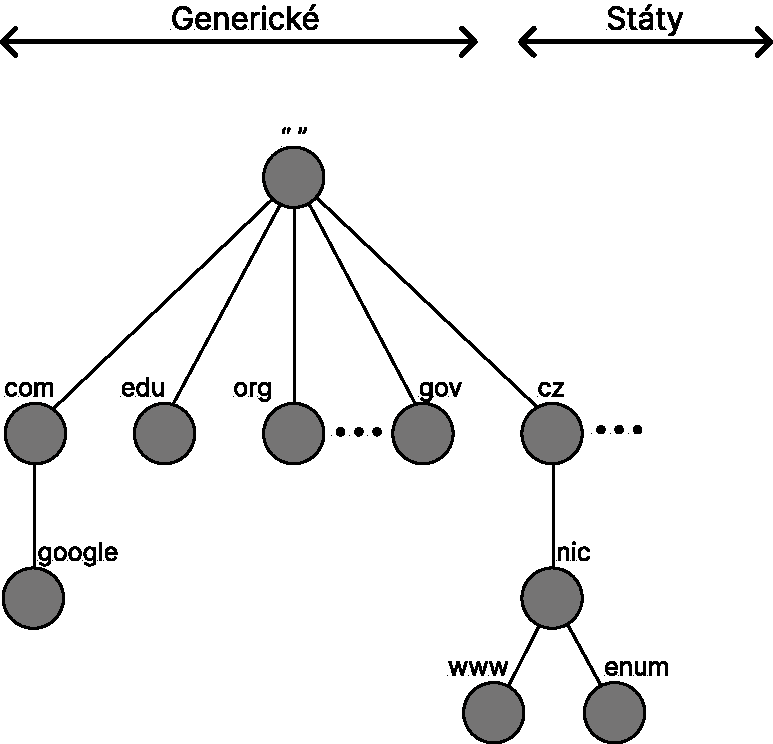
\includegraphics{obrazky-figures/DNS_tree.pdf}
		}
		\caption{DNS strom}
		\label{fig:dns_tree}
\end{figure}

% DNS records
\subsection{Typy záznamů} \label{subsec:DNS_records}
Služeb, které \Gls{DNS} poskytuje, je více, avšak na samotnou detekci je zvolena pouze část z~dostupných. Díky dostupnosti a~veřejnosti dat v~\Gls{DNS} dotazu je možné tyto služby odchytávat a~získávat z~nich potřebná data~\cite{RFC1035}. Níže jsou zmíněné ty, které jsou v~mé práci přínosné pro detekci škodlivosti.

% a~record
\subsubsection{Záznam typu A~-- IP Address} \label{subsubsec:Record_A}
Jedná se o~nejzákladnější typ \Gls{DNS} záznamu. Díky němu je možné spojit danou doménu se samotnou IP adresou serveru. Je v~něm uložená IP adresa ve formě IPv4, což je 32~bitové číslo dělené po osmi bitech (tzv. oktetech). Příklad IPv4 adresy může být například \uv{147.229.9.23}, což je adresa pro \uv{www.fit.vutbr.cz}.
Lze ji získat mnoha způsoby, kdy jedním z~nich je \verb|dig a~+short www.fit.vutbr.cz|.

% AAAA record
\subsubsection{Záznam typu AAAA -- IPv6 Address} \label{subsubsec:Record_AAAA}
S~problémem úbytku IPv4 adres se museli rozšiřovat adresy typu IPv6. Server může mít oba typy záznamů (A~i~AAAA), ale stačí mu jen jeden z~nich. Tento typ záznamu je zcela stejný jako záznam typu~A, s~jediným rozdílem a~tím je forma IP adresy, 128~bitů. Příkladem IPv6 adresy by mohlo být například \uv{2001:67c:1220:809::93e5:917}, což je adresa pro \uv{www.fit.vutbr.cz}. Lze ji získat, jako i~ostatní záznamy, mnoha způsoby, kdy jedním z~nich je \verb|dig AAAA +short www.fit.vutbr.cz|.

% CNAME record
\subsubsection{Záznam typu CNAME -- Canonial Name} \label{subsubsec:Record_CNAME}
Ve zkráceném vysvětlení se jedná o~překlad aliasů počítačů. Neboli na jedné IP adrese může fungovat 1 či více poddomén. Vždy se tyto záznamy mapují na oficiální (kanonické) jméno. Toto se dá využít například při přetížení serveru, kdy změníme alias tak, že se vše odkazuje na záložní server. Pokud je tento záznam nastaven, lze ho získat například z~příkazu \verb|dig CNAME +short fit.vutbr.cz|

% MX record
\subsubsection{Záznam typu MX -- Mail Exchanger} \label{subsubsec:Record_MX}
Udává adresu a~prioritu serveru pro přijímaní elektronické pošty pro danou doménu. Při získání MX záznamu si můžeme povšimnout dvou parametrů -- přirozené číslo, které značí prioritu (čím menší číslo, tím větší priorita), a~doménové jméno serveru. Lze vyčíst například z~\verb|dig MX +short fit.vutbr.cz|. 

% NS record
\subsubsection{Záznam typu NS -- Name Server} \label{subsubsec:Record_NS}
V~tomto typu záznamu můžeme najít autoritativní \Gls{DNS} server pro danou doménu, na kterém jsou uloženy \Gls{DNS} záznamy. I~zde je vhodné mít primární a~sekundární server (může jich být více), kdy při výpadku může fungovat druhý server. Všechny autoritativní servery si můžeme zobrazit pomocí příkazu \verb|dig NS +short fit.vutbr.cz|, kde však nezjistíme, který je primární. Pokud bychom chtěli zjistit, jaký je primární server, tak bychom se museli podívat do SOA záznamu, kterým se zabývám v~následující podsekci.

% SOA record
\subsubsection{Záznam typu SOA -- Start Of Authority} \label{subsubsec:Record_SOA}
Obsahuje informace týkající se uložení autoritativních dat pro danou zónu, kdy každá zóna obsahuje právě jeden záznam SOA. Nachází se v~něm adresa primárního serveru a~adresa elektronické pošty jeho správce, kde v~adrese elektronické pošty je však nahrazen zavináč za tečku. Záznam obsahuje další prvky, kterými jsou:
\begin{itemize}
    \item \texttt{SERIAL} -- je třeba zvětšit při každé změně v~záznamu, aby sekundární server zaregistroval změnu,
    \item \texttt{REFRESH} -- jak často se má sekundární server ptát na změnu v~zónovém souboru,
    \item \texttt{RETRY} -- v~jakých intervalech se má při neúspěchu dotazovat znovu,
    \item \texttt{EXPIRE} -- po jak dlouhé době označí sekundární server data jako neaktuální, pokud se mu nepodařilo kontaktovat primární server,
    \item \texttt{\Gls{TTL}} -- doba platnosti záznamů.
\end{itemize}
Tento typ záznamu si můžeme zobrazit pomocí příkazu \verb|dig SOA +short fit.vutbr.cz|.

% TXT record
\subsubsection{Záznam typu TXT} \label{subsubsec:Record_TXT}
Zde jsou uchována dodatečné informace k~dané doméně, serveru, správci apod. daného uzlu ve stromu \Gls{DNS}.
Slouží pro vkládání jednoduchého textu do záznamu \Gls{DNS}.

Pro ověřování, zda je daná doména validní se zde využívají také 3 typy záznamů pro validaci~\cite{RFC7489}:
\begin{itemize}
    \item \textbf{SPF} (Sender Policy Framework) -- obsahuje seznam všech autorizovaných serverů, které mají povolení posílat email zprávy z~této domény,
    \item \textbf{DKIM} (Domain Keys Identified Mail) -- slouží pro elektronické podepisování kombinací privátního a~veřejného klíče. Slouží tedy k~ověření, že email je z~domény, z~které má být. Veřejný klíč asociovaný k~dané doméně je uložen také v~TXT záznamu,
    \item \textbf{DMARC} (Domain-based Message Authentication, Reportin \& Conformance) -- slouží k~rozhodování v~případě, že daný email neprojde. Pak se zde rozhodne, zda-li bude puštěn dále, dán do karantény nebo odmítnut.
\end{itemize}

% DNSSEC
\subsection{Zabezpečení záznamů DNS pomocí DNSSEC} \label{subsec:DNSSEC}
Protokol \Gls{DNS} byl navržen tak, aby byl rychlý a~jednoduchý, proto v~tomto protokolu nebylo zahrnuto téměř žádné zabezpečení. V~dřívějších dobách byl internet používán menší skupinkou lidí, kde nedocházelo ke kybernetickým útokům. Pro danou dobu byla důležitá rychlost a~efektivita, která byla potřebná na starších a~méně výkonných počítačích. 

V~moderní době však lidé zažívají čím dál tím častěji kybernetické útoky, které mají v~mnohých případech velké následky, ať už se jedná o~finanční či psychické. Útočník při překladu doménového jména podstrčí falešnou IP adresu, a~tak si převede oběť na svoji stránku, kde od ní může získat veškerá data. Takto se i~přes správné zadání domény oběť ocitne na falešné stránce, kterou jí podvrhl útočník. Pro větší zabezpečí a~omezení těchto útoků vzniklo rozšíření po zkratkou \Gls{DNSSEC}.

Je to zkratka anglického slova Domain Name System Security Extensions, což je technologie, která využívá k~ověřování původu dat v~\Gls{DNS} záznamu pomocí elektronického podpisu. Díky tomuto je uživatel schopný ověřit, zda data, která dostal, jsou pravá nebo se jedná o~podvrh.

Toto zabezpečení podepisuje soukromým klíčem \Gls{DNS} serveru, kdy samotný podpis je uložen v~záznamech RRSIG a~veřejný klíč v~záznamu DNSKEY, které jsou součástí zónových souborů. Podepisování funguje na principu tzv. řetězec autority, kdy pravost veřejného klíče potvrzuje vždy nadřazená autorita pomocí záznamu DS~\cite{DNS_Matousek, RFC4034}.

% WHOIS and RDAP
\section{WHOIS a~RDAP} \label{sec:WHOIS_RDAP}
Tyto protokoly poskytují informace o~subjektech na internetu. Mohou poskytovat informace jako například:
\begin{itemize}
    \item registrátor domény,
    \item vlastník domény,
    \item datum registrace domény,
    \item stav a~datum platnosti registrace domény,
    \item kontaktní údaje,
    \item dodatečné informace o~IP adrese.
\end{itemize}

% WHOIS
\subsection{WHOIS} \label{subsec:WHOIS}
WHOIS (není to zkratka, jen se tento název píše kapitálkami) je protokol dotazů a~odpovědí. Byl zaveden v~roce 1982 a~používá se k~dotazování do databáze o~registrátorech či majitelích IP adres nebo domén, ale také o~autonomních systémech~\cite{RFC3912}. Probíhá pomocí TCP\footnote{TCP -- Transmission Control Protocol} komunikace na portu 43 na základě komunikace klient-server. 

Protože bezpečnost je v~tomto protokolu velmi slabá, slouží pouze k~ukládání veřejných záznamů, které nejsou citlivého charakteru. Využívá se tedy k~předávání zejména veřejně dostupných záznamů, u~kterých není vysoká pravděpodobnost poškození dané osoby.
Samotné odesílání i~dotazování je posíláno v~podobě prostého textu, které jsou čitelné pro běžného člověka. Tímto způsobem jsou ukládány i~v~samotné databázi.  

Při vytvoření doménového jména musí její majitel odeslat své údaje organizaci ICANN (Internet Corporation for Assigned Names and Numbers). Ta z~nich danou část zveřejní do veřejné databáze WHOIS a~lze se k~nim dostat například přes dotaz WHOIS nebo z~našeho vyhledávače. Dále musí majitel aktualizovat veškeré změny, které jsou s~jeho doménou spojené, aby udržoval informace aktuální a~platné. Pokud nezadá platné údaje, nebo žádné, tak doména může být pozastavena či úplně smazána~\cite{icann_whois}.

% WHOIS Privacy
\subsection{Osobní data v~dotazu WHOIS} \label{subsec:WHOIS_privacy}
Osobní data mohou být z~části skryta skrz ochranu osoby. Proto se k~těmto účelům používá maskovaní WHOIS, kdy se veškerá data převedou na právnickou osobu, která zastupuje danou osobu. Tudíž tato právnická osoba pak vystupuje jako vlastník domény. 

Tento způsob se nazývá v~angličtině jako WHOIS Privacy nebo Domain Privacy a~ve většině případech registrátoři tento způsob využívají. Avšak i~přes tyto možnosti jsou stále některé, které tuto variantu neumožňují.

% RDAP
\subsection{RDAP} \label{subsec:RDAP}
\textit{Registration Data Access Protocol (\Gls{RDAP})} je nástupcem protokolu WHOIS. Stejně jako WHOIS poskytuje tento protokol přístup k~informacím o~internetových zdrojích, ale ukládá je ve strukturované podobě. Nabízí však rozšíření, která zlepšují nedostatky předchozího protokolu. Mezi ně je možno zařadit podpora internacionalizace, možnost poskytovat diferencovaný přístup k~registračním údajům, ale mezi ty nejdůležitější patří zabezpečení přístupu k~datům.

\Gls{RDAP} pracuje nad protokolem HTTP\footnote{HTTP -- Hypertext Transfer Protocol}, díky kterému používá stejné stavové návratové kódy. Proto například dochází k~přesměrování na jiný odkaz, pokud ten zná odpověď na daný dotaz~\cite{RFC7480}.

Formát odpovědi z~dotazu \Gls{RDAP} se liší oproti odpovědi z~WHOIS. První zmíněný má doporučený JSON\footnote{JSON -- JavaScript Object Notation} formát s~definovaným schématem, kdežto druhý má odpověď pouze ve formě prostého textu~\cite{RFC9083}.

% RDAP data
\subsection{Data získaná z~dotazu RDAP} \label{sec:RDAP_data}
Struktura odpovědi má předem jasná pravidla, v~jakém formátu se má vrátit a~co má obsahovat.
Odpověď na \Gls{RDAP} dotaz o~doméně obsahuje jméno ve forme LDH (Letter, Digit, Hyphen), datum a~čas registrace i~expirace domény a~také časové razítko poslední aktualizace databáze. Je zde možné zobrazit datum i~čas poslední úpravy, ale to je možné jen v~případě, že daná doména byla od vytvoření nějak upravena. Mezi další povinné údaje patří informace o~registrátorovi, přesněji jeho údaje definované pomocí vCard. Mezi ně lze zařadit například IANA ID~\cite{RFC9083, RFC8605}.

Dané informace mohou být skryté, podobně jako v~podsekci~\ref{subsec:WHOIS_privacy}, pokud by to poškozovalo danou osobu a~nebo nebyl vydán souhlas s~jejich zveřejněním.

% Secured communication
\section{Zabezpečená komunikace} \label{sec:Secured_communication}
Bezpečný pohyb na internetu je možné také kontrolovat pomocí kontroly důvěryhodnosti domén. Je obecně známo, že díky koncovce S~v~HTTPS\footnote{HTTPS -- Hypertext Transfer Protocol Secure} se cítí člověk při kliknutí na doménu mnohem bezpečněji než při běžném HTTP. Jedná se o~ochranu integrity dat uživatelů při pohybu na internetu, kdy HTTPS je HTTP protokol s~šifrováním přenesených dat pomocí protokolu \Gls{TLS} (Transport Layer Security). \Gls{TLS} certifikáty slouží pro zabezpečení služeb jako například WWW, elektronické pošty a~jiné. Díky tomuto je snaha omezovat výskyt infikovaného obsahu na těchto stránkách~\cite{durumeric2017security}.

% Evolution of secured communication
\subsection{Vývoj zabezpečené komunikace} \label{subsec:Evolution_of_secured_communication}
Aktuálně používaný \Gls{TLS} protokol ve verzích 1.2 a~1.3 vznikl z~původního SSL (Secure Sockets Layer) protokolu. Původní SSL protokol byl navržen společností Netscape Communications, ale tato verze se šířila pouze uvnitř společnosti, protože měla několik nedostatků a~chyb. Byl velmi náchylný proti útokům skrze jeho jednoduchou kontrolu namísto kryptografické silné hašovací funkce. Proto až po vylepšení vyšla verze 2.0, která byla již publikována~\cite{oppliger2009ssl, 10.1007/978-3-030-57043-9_25}.

S~neustálým rozvojem však bylo toto zabezpečení nedostačující a~vzniklo \Gls{TLS}, které nyní je podporováno ve verzi 1.2, ale nejaktuálnější a~nejbezpečnější z~nynějšího pohledu je ve verzi 1.3. To oproti starší verzi změnilo především šifrovaní a~bezpečnější přenos veškerých zpráv, a~to i~při vytváření prvotního spojení~\cite{RFC8446}, ale také mnohem rychlejší prvotní propojení~\cite{10.1145/3442381.3450057}.

Avšak i~přes novější verze se stále v~některých případech používají starší verze, nebo dokonce i~v~řadách SSL, které však jsou pro útočníky přívětivým prostředím vzhledem k~malému a~neodpovídajícímu zabezpečení pro dnešní typy útoků. V~některých odvětvích je ale už předem striktně zakázáno, které protokoly nejsou dostačující, jako například při placení kartami je přikázáno používat \Gls{TLS} verze 2.0 a~výš~\cite{industry2010data}.

% Certificates and chains of trust
\subsection{X.509 certifikáty a~řetězce důvěry} \label{subsec:Certificates_and_chains_of_trust}
Na internetu jsou certifikáty ekvivalentem úředních dokumentů. Obsahují informace o~vydavateli, subjektu a~jeho veřejném klíči. Digitální podpis vydavatele chrání všechny tyto informace a~díky propojení identity s~veřejným klíčem je možné tento veřejný klíč použít pro identifikaci této digitální identity.

% Certificates
\subsubsection{X.509 certifikáty} \label{subsubsec:Certificates}
X.509 verze 3 je standardem pro certifikáty a~jsou veřejně dostupné na internetu. Jak takový certifikát vypadá jeho strukturou je znázorněno na obrázku~\ref{fig:X.509_certificate}. Je zde sériové číslo certifikátu, jakým algoritmem je šifrováno, informace o~vydavateli (\textbf{C} -- stát, \textbf{S} -- stát v~Americe, \textbf{L} -- město, \textbf{O} -- jméno organizace, \textbf{CN} -- jméno instance),
datum platnosti, informace o~vlastníkovi certifikátu, veřejný klíč a~rozšíření, kde najdeme jaká povolení jsou spojena při zacházení s~tímto certifikátem~\cite{RFC3280}.

Z~certifikátu je možné zjistit, jak se má s~daným klíčem zacházet a~omezení daného certifikátu, pro které jmenné prostory může daná certifikační autorita vydávat certifikáty a~v~poslední řade můžeme zjistit alternativní jména vydavatele a~certifikovaného subjektu (\Gls{DNS} doména, IP adresa atd.)~\cite{10.1007/978-3-030-57043-9_25}.

\begin{figure}[H]
    \centering
		\scalebox{0.3}{
			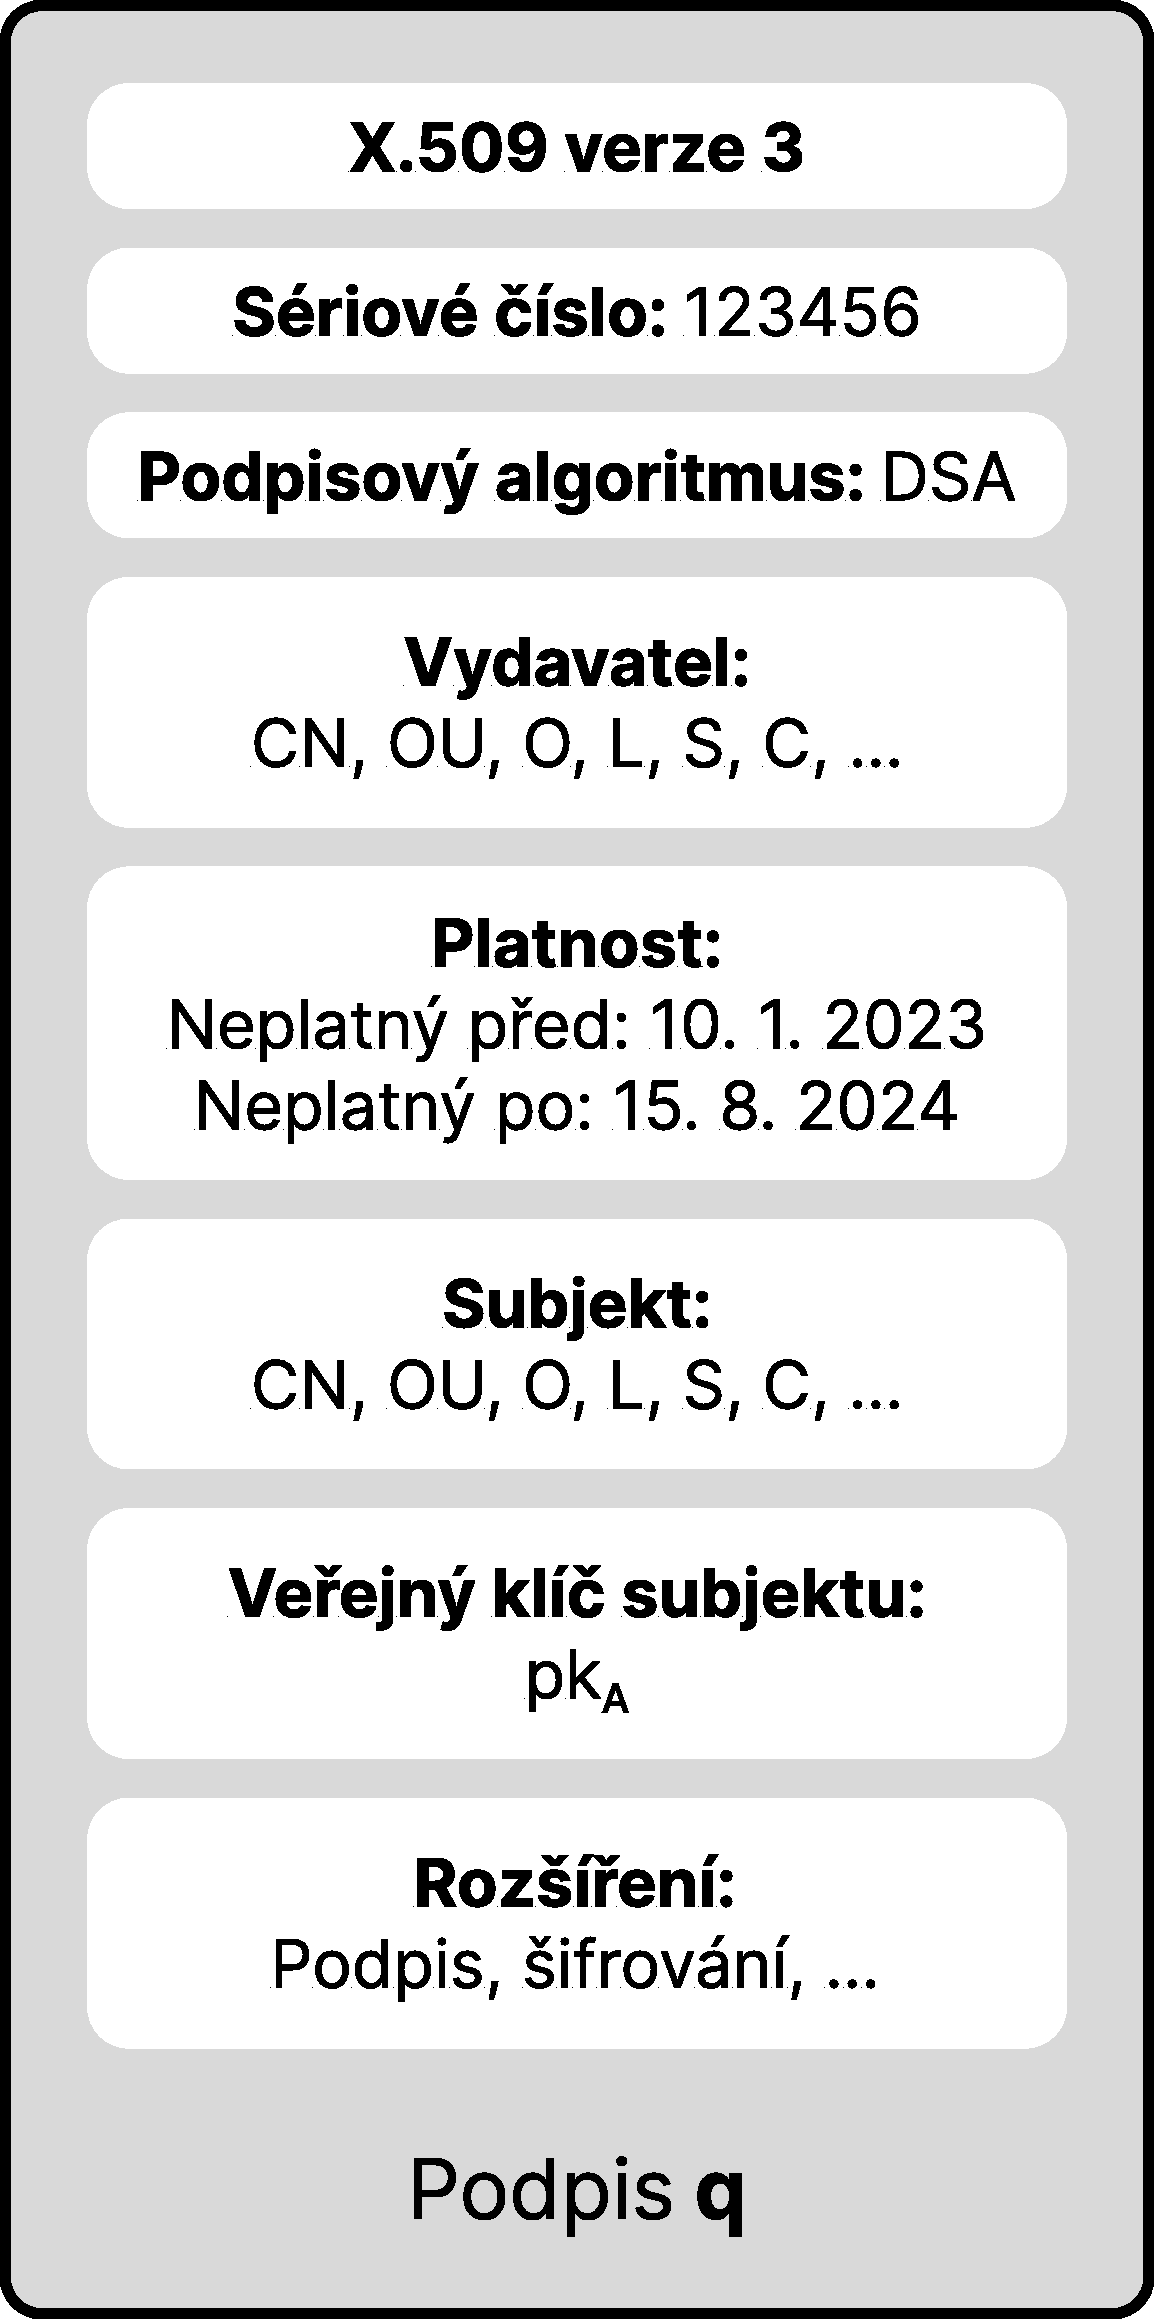
\includegraphics{obrazky-figures/X.509_certificate.pdf}
		}
		\caption{Struktura X.509 certifikátu}
		\label{fig:X.509_certificate}
\end{figure}

% Chains of trust
\subsubsection{Řetězce důvěry} \label{subsubsec:Chains_of_trust}
Ověření pravosti a~důvěryhodnosti daného certifikátu je možné díky řetězci důvěry těchto certifikátů. Na počátku jsou kořenové certifikáty, které podepisuje a~vydává sama certifikační autorita (dále jako CA). Tyto certifikáty lze ověřit pouze tím, že každý klient má ve svém počítači nebo prohlížeči uložen seznam těchto kořenových autorit.
Dále v~tomto řetězci figurují mezistupně, kterých může být několik. Fungují jako mezistupeň mezi kořenovou CA a~koncovým certifikátem. Tento certifikát je podepsán kořenovou CA, ale koncový certifikát podepisuje on sám svým soukromým klíčem. 

Odkaz na vydavatele se uloží v~certifikátu, aby bylo jasné, kdo daný certifikát podepsal a~na koho se odkazovat. Již zmíněné podpisy pak slouží pro ověření již zmíněné pravosti certifikátu, což docílíme kontrolou podpisu přes veřejný klíč nadřazeného certifikátu~\cite{https://doi.org/10.1002/sec.198}. Příklad řetězce důvěry můžeme vidět na obrázku~\ref{fig:CA_chain_of_trust}.

\begin{figure}[H]
    \centering
		\scalebox{0.3}{
			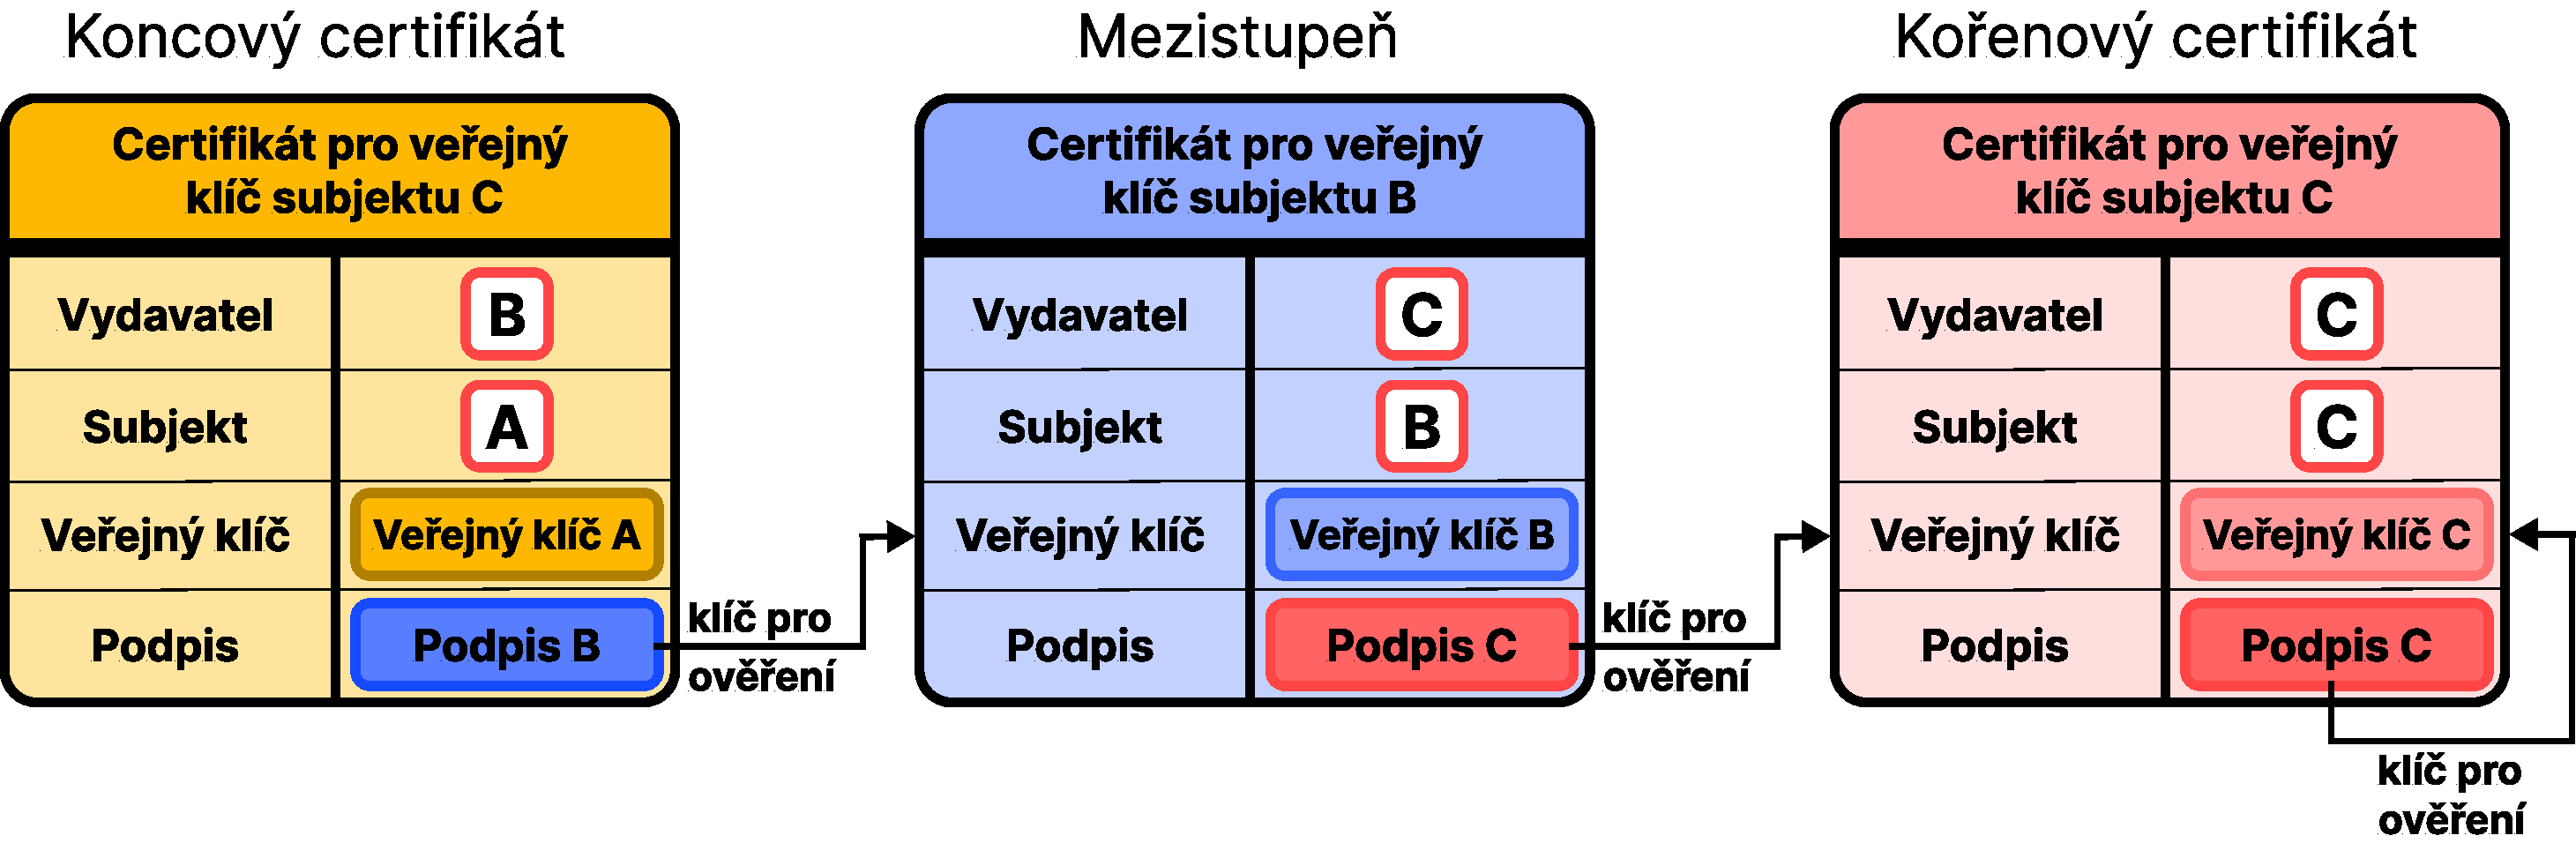
\includegraphics{obrazky-figures/CA_chain.pdf}
		}
		\caption{Příklad řetězce důvěry}
		\label{fig:CA_chain_of_trust}
\end{figure}

% Geolocation 
\section{Geolokační údaje} \label{sec:Geolocation}
Informace o~geografické poloze se typicky zjišťují pro každou IP adresu, která zastupuje samotné zařízení, jenž je připojeno do internetu. Dané informace se mohou lišit, tudíž ať už se jedná pouze o~lokaci, ve kterém státě se nachází nebo až pro přesné souřadnice.

% Location from RDAP
\subsection{Lokace získaná z~RDAP} \label{subsec:Location_RDAP}
Některé informace o~lokaci dané domény je možné získat ze samotného dotazu \Gls{RDAP}. Ten však obsahuje pouze zlomek informací, které bychom potřebovali vědět pro přesnější lokalizaci a~to přesněji pouze státě, ve kterém se IP adresa nachází~\cite{RFC9083}. Pomocí \Gls{RDAP} lze však získat přesnější informace nejen díky IP adrese.

Údaje o~registrátorovi a~vlastníkovi domény mohou v~sobě obsahovat často i~kontaktní údaje, ve kterých může být součástí adresa. Avšak v~tento moment je důležité myslet na to, že registrátor nemusí a~často nutně nesouvisí s~vlastníkem této domény. Proto dané kontaktní údaje nemusí souhlasit s~registrujícím, natož pak lokace pevných zařízení. Veškeré údaje registrujícího, včetně geolokačních, už jsou pro nás více relevantní, ačkoliv zde stejně musíme být více obezřetní, že nemusí zcela souviset s~lokací dané IP adresy~\cite{Geolocation_whois}. Často jsou i~tato data skryta v~zájmu uchování a~ochraně soukromí daných osob, viz podsekci~\ref{subsec:WHOIS_privacy}.

Tyto údaje nám však mohou sloužit pro porovnání s~informacemi získanými z~databází zmíněných v~další podsekci. Mohou také sloužit jako záložní údaj, pokud se v~databázi daná IP adresa nevyskytuje nebo jen k~ní nejsou přidělené údaje.

% Geolocation_database
\subsection{Geolokační databáze} \label{subsec:Geolocation_database}
Existuje mnoho těchto typů databází, které ukládají geolokační údaje IP adres. Mezi ně můžeme zařadit například MaxMind GeoIP2, ipgeolocation nebo db-ip. Poskytují často mnohem rozsáhlejší informace a~přesnější údaje lokace včetně souřadnic.

Často tyto služby jsou zpoplatněné a~nevyhovují pro účel této práce. Mají například omezen počet dotazů, což znemožňuje práci ve velkém měřítku. Proto je vybrána verze GeoIP2, přesněji její verze GeoLite~\cite{maxmindGeoLite2Free}. Na tyto databáze se lze dotazovat a~stahovat je lokálně.

Takto získaná data mohou sloužit pro detekci škodlivých domén, kdy například může někde vzniknout ohnisko poskytovatelů těchto domén a~proto je velmi velká pravděpodobnost, že pokud se objeví nějaká IP adresa na tomto místě, tak bude také škodlivá. 

%-----------------------------------------------------
% Resources for classify
\chapter{Nástroje pro klasifikaci} \label{chap:Classification}
V~této kapitole je podrobněji rozebrána nejdůležitější část práce, detekce pomocí klasifikátorů. Tyto algoritmy fungují na základě vytváření kolekce rozhodovacích stromů, kdy každý následující strom dělá korekci předchozích stromů pro nejlepší výsledek. Výsledek tohoto procesu je tedy sumarizací výsledků všech stromů. Příklad jednoduché kolekce je ukázán na obrázku~\ref{fig:decision_tree_image}.
\begin{figure}[H]
    \centering
		\scalebox{0.3}{
			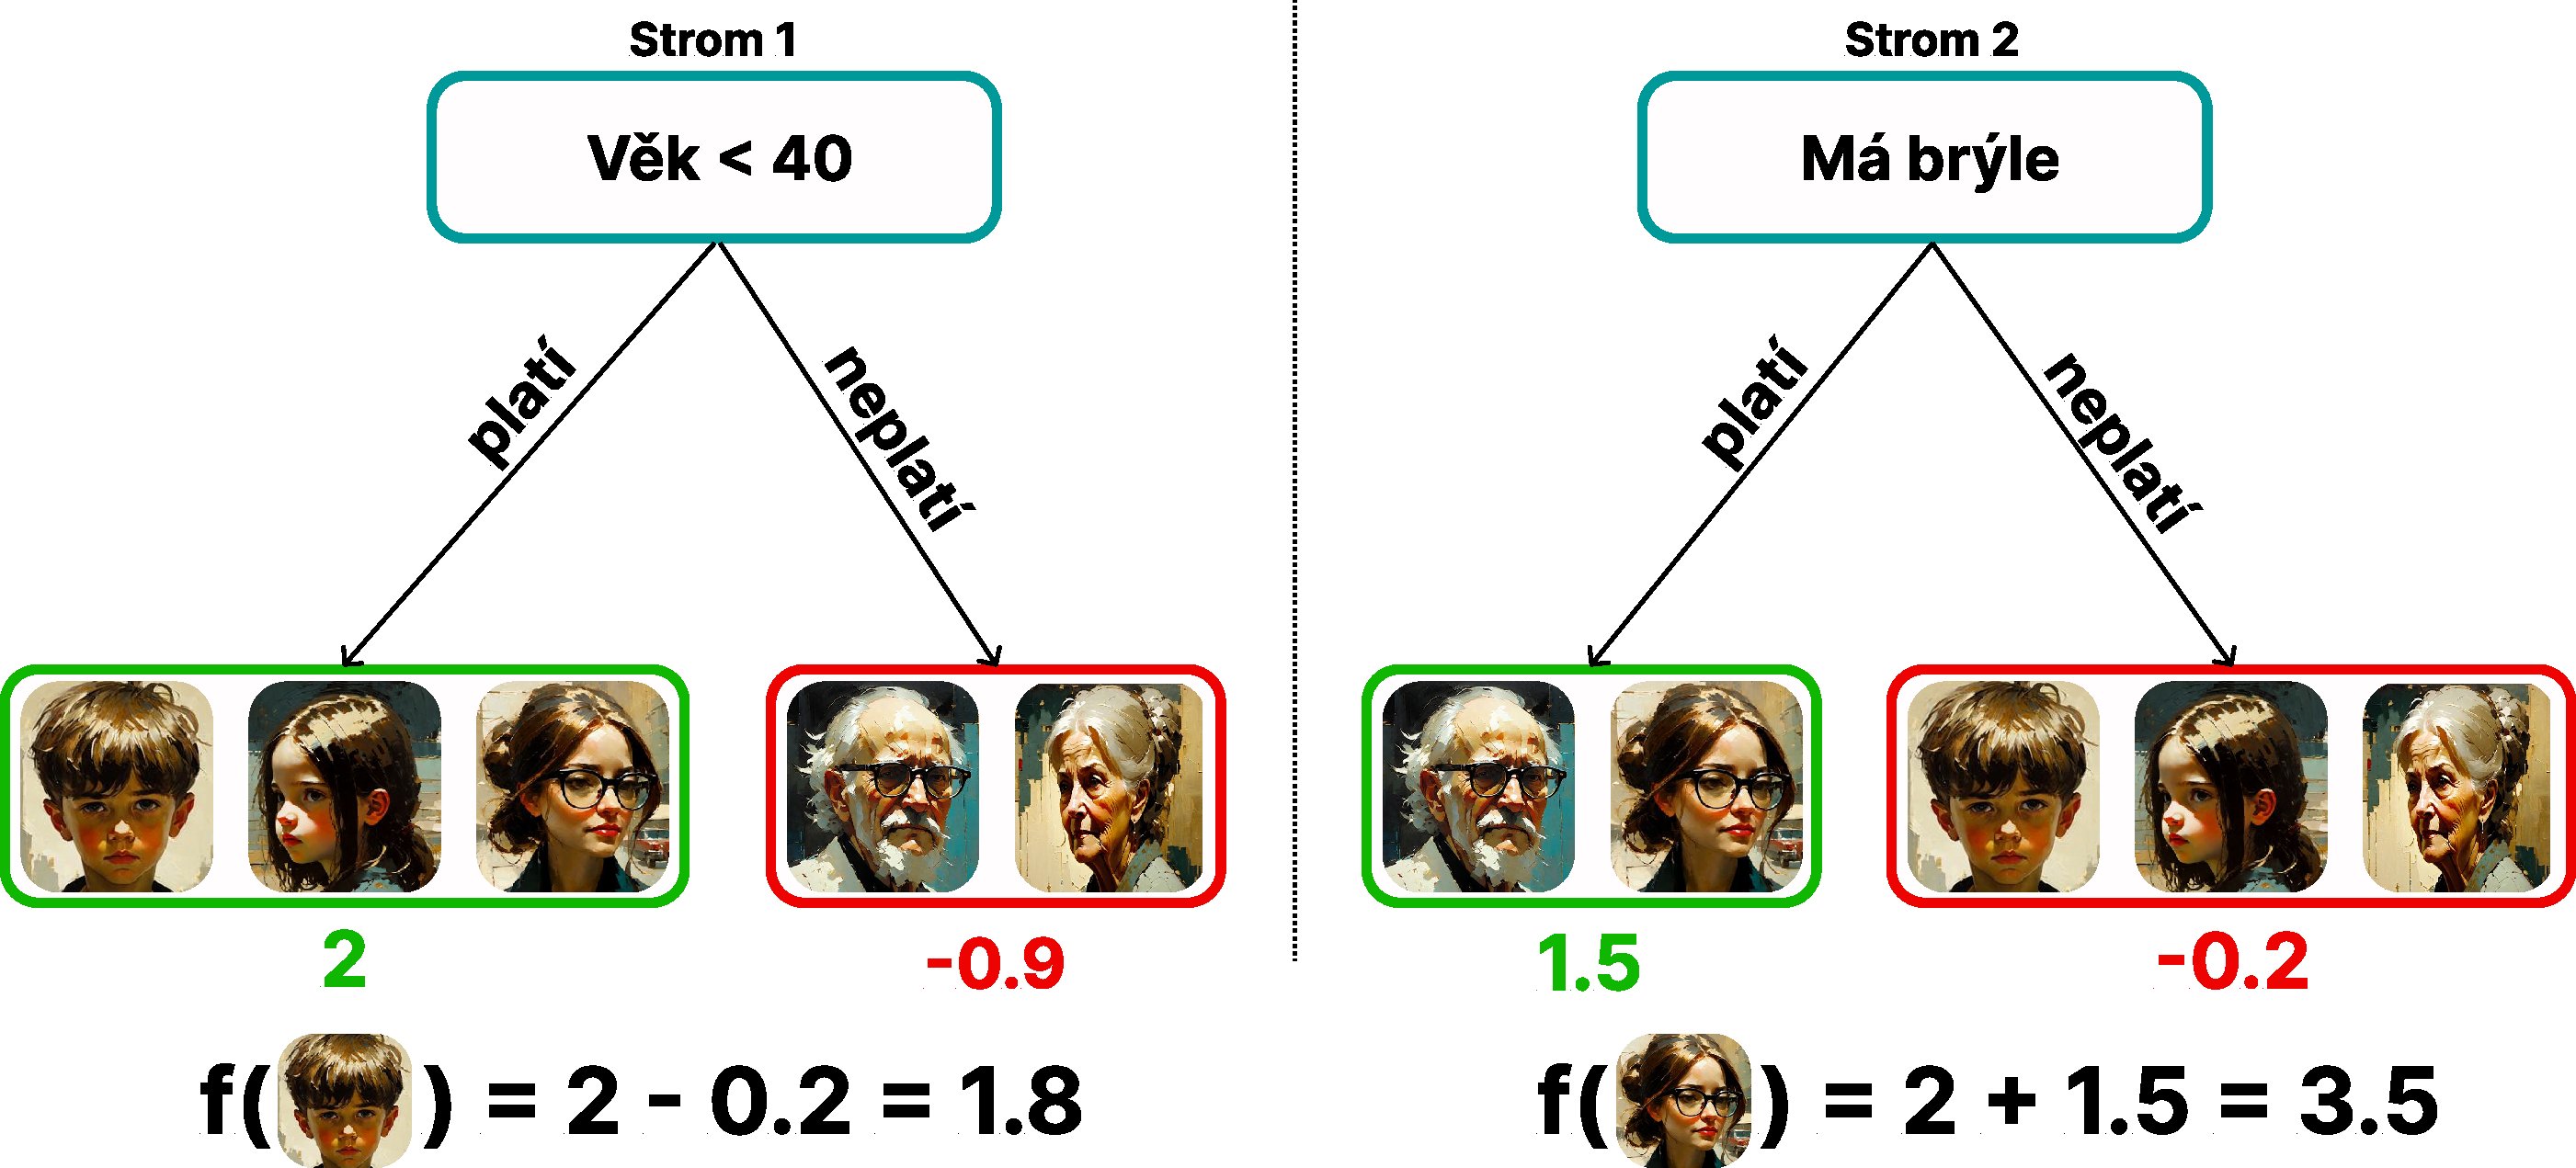
\includegraphics{obrazky-figures/decision.pdf}
		}
		\caption{Příklad stromového rozhodování, kdy každý strom má vlastní rozhodovací podmínky. Výsledek předpovědi je součet všech stromů.}
		\label{fig:decision_tree_image}
\end{figure}
\noindent Následující pojmy definují správné nebo špatné detekce v~modelu, kdy však jako negativní výsledek je považována první třída, v~mém případě benigní.
\begin{itemize}
    \item \textbf{Skutečně pozitivní výsledky (True Positives)} -- kladný výsledek detekován jako kladný,
    \item \textbf{Falešně pozitivní výsledky (False Positives)} -- záporný výsledek detekován jako záporný,
    \item \textbf{Skutečně negativní výsledky (True Negatives)} -- kladný výsledek detekován jako záporný,
    \item \textbf{Falešně negativní výsledky (False Negatives)} -- záporný výsledek detekován jako kladný.
\end{itemize}
A~díky nim je možné vytvořit matici záměn, viz tabulku~\ref{tab:confusion_matrix}, ve které se nacházejí všechny zmíněné pojmy. Je možné si v~ní všimnout, že co nejvíce hodnot očekáváme v~levém horním a~v~pravém dolní rohu, což pak značí kvalitní model s~velkou úspěšností predikce. Označuje to stav, kdy aktuální predikovaná doména odpovídá svým typem predikci typu, který provedl model.
\begin{table}[htbp]
  \centering
  \begin{tabular}{|l|c|c|}
    \hline
    \multicolumn{1}{|c|}{\multirow{2}{*}{\textbf{Aktuální}}} & \multicolumn{2}{c|}{\textbf{Predikce}} \\
    \cline{2-3}
                     & \textit{Benigní} & \textit{Malware} \\
    \hline
    \textit{Benigní} & True Negatives & False Positives \\
    \hline
    \textit{Malware} & False Negatives & True Positives \\
    \hline
  \end{tabular}
  \caption{Matice záměn natrénovaného modelu}
  \label{tab:confusion_matrix}
\end{table} \\
Následně ve výsledku získáme hodnoty, které lze definovat matematickými výpočty. Řadíme mezi ně \textbf{Accuracy}, \textbf{Precision}, \textbf{Recall} a~\textbf{skóre F1}. Tyto výpočty jsou specfikované pro binární klasifikace, která je využita v~této práci.
\begin{align*}
    \textbf{Accuracy} &= \frac{\text{Počet správných predikcí}}{\text{Celkový počet predikcí}} \\[10pt]
    \textbf{Precision} &= \frac{\text{True Positives}}{\text{True Positives + False Positives}} \\[10pt]
    \textbf{Recall} &= \frac{\text{True Positives}}{\text{True Positives + False Negatives}} \\[10pt]
    \textbf{Skóre F1} &= 2 \times \frac{\text{Precision} \times \text{Recall}}{\text{Precision + Recall}}
\end{align*}

Accuracy je vhodná pro vyvážené datové sady, skóre F1 naopak pokud jedna datová sada je většího počtu. Precision se zaměřuje na True Positives a~pomáhá snižovat hodnotu False Positives. Naopak Recall se zaměřuje na co nejvíce pozitivních výsledků a~pomáhá eliminovat False Negatives.

% Scikit-Learn
\section{Scikit-Learn} \label{sec:Scikit_Learn}
Scikit-Learn nebo také zkráceně \texttt{sklearn} je volně dostupná knihovna pro strojové učení v~jazyce Python. Poskytovanou funkcionalitou je regrese, s~využitím lineární nebo logistické regrese, \textbf{klasifikace}, s~využitím například K-Nearest Neighbors, clustering, využívajíc K-Means nebo K-Means++, model selection a~také preprocessing, například možností metody Min-Max normalizace.~\cite{scikit-learn}

% Classifiers
\section{Přehled klasifikátorů} \label{sec:Classifiers}
V~této bakalářské práci bylo využito mnoho algoritmů strojového učení, zejména na různorodost a~otestování možných výsledků. Zde je výčet a~přiblížení jednotlivých algoritmů.

% Logistic Regression
\subsubsection{Logistická regrese (Logistic Regression)} \label{subsubsec:Logistic_Regression}
Jedná se o~statistický model, který má za úkol odhadovat pravděpodobnosti, zda daná instance patří do určité třídy či nikoliv. Algoritmus logistické regrese využívá koncept logistické funkce, známá také jako funkce sigmoid, která mapuje libovolné reálné číslo na pravděpodobnostní hodnotu mezi 0 a~1. Tato funkce se využívá k~předpovědi pravděpodobnosti výskytu dané události, kde samotná událost je definována závislou proměnnou, která je také binární~\cite{Logistic_regression}.

% SVM
\subsubsection{Support Vector Machine (SVM)} \label{subsubsec:SVM}
Support Vector Machine, neboli také SVM, je výkonný algoritmus strojového učení, který se používá pro lineární nebo nelineární klasifikaci a~regresi. SVM lze použít pro řadu úloh, jako je klasifikace textu, klasifikace obrázků, detekce spamu, identifikace rukopisu, analýza genové exprese, detekce obličejů a~detekce anomálií. SVM jsou přizpůsobivé a~efektivní v~různých aplikacích, protože si poradí s~daty o~velkém rozměru a~nelineárními vztahy~\cite{SVM}.

% Decision tree
\subsubsection{Rozhodovací strom (Decision Tree)}
Ačkoliv v~programování se jedná o~algoritmus, názornější vysvětlení je lepší podat způsobem, že rozhodovací strom je stromová struktura podobná diagramu, kde každý vnitřní uzel označuje funkci, větve označují pravidla a~listové uzly označují výsledek algoritmu~\cite{Decision_tree}.
Příklad takového rozhodovacího stromu lze vidět i~na jednoduchém příkladu, jako je na obrázku~\ref{fig:decision_tree_image}.

% Random Forest
\subsubsection{Náhodný les (Random Forest)} \label{subsubsec:Random_Forest}
Tento klasifikátor je metoda skupinového učení pro klasifikaci, regresi a~další úlohy, která funguje tak, že v~době trénování vytváří mnoho rozhodovacích stromů. U~klasifikačních úloh je vybrán výsledek, který byl vybrán nejvíce stromy. Naopak u~regrese je zprůměrován výsledek všech stromů. Klasifikátory Random Forest napravují zvyk rozhodovacích stromů příliš se přizpůsobovat trénovací množině~\cite{RandomForest}.

% AdaBoost
\subsubsection{AdaBoost} \label{subsubsec:AdaBoost}
\textit{Adaptive Boosting} je statistický klasifikační meta algoritmus. Lze jej použít ve spojení s~mnoha dalšími typy učebních algoritmů a~zlepšit tak výkon. Výstupy ostatních učících se algoritmů (\uv{slabých učících se algoritmů}) se spojí do váženého součtu, který představuje konečný výstup zesíleného klasifikátoru.

AdaBoost je adaptivní v~tom smyslu, že následné slabé klasifikátory jsou upraveny ve prospěch těch případů, které byly předchozími klasifikátory špatně klasifikovány. Zároveň v~některých problémech může méně podléhat přetrénovaní na rozdíl od ostatních učících se algoritmů~\cite{AdaBoost}.

% XGBoost
\subsubsection{XGBoost} \label{subsubsec:XGBoost}
\textit{Extreme Gradient Boosting package}, neboli zkráceně XGBoost, je open-source knihovna, která poskytuje gradientní boosting framework pro jazyky C++, Java, Python, R, Julia, Perl a~Scala. Cílem je poskytnout škálovatelnost, přenosnou a~distribuovanou knihovnu pro gradientní posilování~\cite{XGBoost}.

% LightGBM
\subsubsection{LightGBM} \label{subsubsec:LightGBM}
\textit{Light gradient-boosting machine} je bezplatný open-source distribuovaný gradient-boostovací framework pro strojové učení. Je založen na algoritmech rozhodovacích stromů a~používá se pro řazení, klasifikaci a~další úlohy strojového učení. Vývoj se zaměřuje na výkon a~škálovatelnost. Mezi jeho hlavní výhody patří rychlost, malé zatížení grafické karty a~větší přesnost~\cite{LightGBM}.

% K-Nearest Neighbors
\subsubsection{Algoritmus k-nejbližších sousedů (K-Nearest Neighbors)} \label{subsubsec:KNN}
Patří mezi další algoritmus strojového učení, který se využívá v~datové analýze a~strojovém učení. Princip spočívá v~začleňování datových bodů ležících blízko sebe do jedné třídy, což je založeno na předpokladu, že body, co jsou blízko sebe, jsou si navzájem podobné. Podobně funguje i~při přidání nového bodu, kdy se hledá nejbližší bod a~tím přidání do dané třídy~\cite{K_Nearest}.

% CatBoost
\subsubsection{CatBoost} \label{subsubsec:CatBoost}
Jedná se o~open-source knihovnu, která poskytuje gradient-boosting na rozhodovacích stromech, která je možná k~použití například pro klasifikační, regresní a~klasifikační úlohy. CatBoost se liší od jiných algoritmů gradientního posilování, jako jsou XGBoost a~LightGBM, protože CatBoost vytváří vyvážené stromy, které mají symetrickou strukturu~\cite{CatBoost}.

% Model training
\section{Trénování modelů}  \label{sec:Model_training}
Proces natrénovaní klasifikátorů je ve většině případů velmi podobný a~skládá se z~několika kroků. Každý z~kroků se postupně zlepšuje a~zpřesňuje vhledem k~získaným poznatkům v~průběhu trénování na dané sadě dat.
\begin{enumerate}
    \item \textbf{Příprava dat:} Prvním krokem trénování je samotná příprava dat, která probíhá sesbíráním, pročištěním a~úpravou dat pro klasifikátor.
    \item \textbf{Rozdělení dat:} Zde se rozdělí datová sada na část trénovací a~část testovací. Trénovací část slouží k~samotnému trénovaní modelu daného klasifikátoru. Testovací poté slouží pro otestování funkčnosti a~zhodnocení výsledků daného modelu. 
    \item \textbf{Definice modelu:} Model se definuje zadáním hyperparametrů modelu. Mezi ně můžeme řadit rychlost učení, počet stromů a~jiné.
    \item \textbf{Trénování:} Zde probíhá samotné trénování, kdy daný klasifikátor v~průběhu zvyšuje a~snižuje váhy daných stromů na základě získaných informací během tohoto procesu.
    \item \textbf{Vyhodnocení:} Po dokončení trénování se využije již zmiňovaná testovací sada dat, díky které získáme výsledky. Mezi ně řadíme \textit{Accuracy, Precision, Recall} a~skóre F1. 
    \item \textbf{Vylepšení hyperparametrů:} Po zhodnocení výsledků lze upravovat hyperparametry daného klasifikátoru pro lepší a~přesnější výsledky. Lze toho docílit postupnými úpravami a~zkoušením ladění všech parametrů.
\end{enumerate}

% SHAP
\section{Důležitost příznaků} \label{sec:feature_importance}
Důležitost příznaků je velice nezbytnou součástí strojového učení, neboť dovoluje pochopení, jak daný model funguje a~také částečnou analýzu dat. Jejich důležitost poskytuje pohled do toho, jak model vytváří své předpovědi, což umožňuje lépe pochopit a~interpretovat chování modelu. Také je možné díky tomuto zjistit, zda data jsou něčím specifická. Může se stát, že pomocí příznaku je zjištěna chyba, která by vedla ke špatnému natrénování, neboli přetrénování jen na specifických datech.

\subsection{GAIN} \label{subsec:GAIN}
Důležitost rysu se vztahuje k~významu vstupních proměnných při predikci cílové proměnné. GAIN, metoda používaná při výběru prvků, vypočítává důležitost prvků (čím vyšší, tím je příznak důležitější) na základě normalizovaných hodnot zisku, což je zisk dělený součtem zisků. Tato technika se běžně používá v~algoritmech gradientního posilování, jako je XGBoost. Tato metoda je také známá jako Giniho důležitost~\cite{scikit-learn-GradientBoostingClassifier.feature_importances_}.

\subsection{SHAP} \label{subsec:SHAP}
Během trénování modelů ve strojovém učení je nezbytné pochopení, jak velký vliv a~důležitost mají dané příznaky, které jsou využity při samotném trénovaní. K~tomu slouží metoda \textbf{\Gls{SHAP}}, neboli \textit{SHapley Additive exPlanations}, díky které je možné získat hodnoty a~zobrazit grafy celkové důležitosti daného příznaku, nebo také váhu příznaků při rozhodování v~daném pozorování na jednom prvku.

% SHAP values
\subsubsection{Shapleyho hodnoty} \label{subsubsec:SHAP_values} 
Původně myšleno jako jedno ze způsobů rozdělení celkových zisků mezi hráče, za předpokladu, že všichni spolupracují. S~touto myšlenkou přišel v~roce 1951 Lloyd Shapley ve své práci ohledně teorie her~\cite{Shapley_Lloyd}. Až postupem času tato myšlenka přešla i~do jiných odvětví, mezi které je možné zařadit i~strojové učení.

Ve strojovém učení tyto hodnoty přiřazují každému příznaku změnu očekávané predikce modelu při podmínění tímto příznakem. Na obrázku~\ref{fig:SHAP_values} je možné vidět, jak výpočet dané hodnoty \Gls{SHAP} funguje. Hodnoty vysvětlují, jak se dostat ze základní hodnoty $E\left[ f(x) \right]$, která byla předpovězena, za předpokladu, že neznáme žádné příznaky až do aktuálního výstupu $f(x)$. Samotná výsledná hodnota \Gls{SHAP} pak vznikne zprůměrováním hodnot $\phi_{i}$~\cite{Shapley_MachineLearning_graph}.
\begin{figure}[H]
    \centering
		\scalebox{0.65}{
			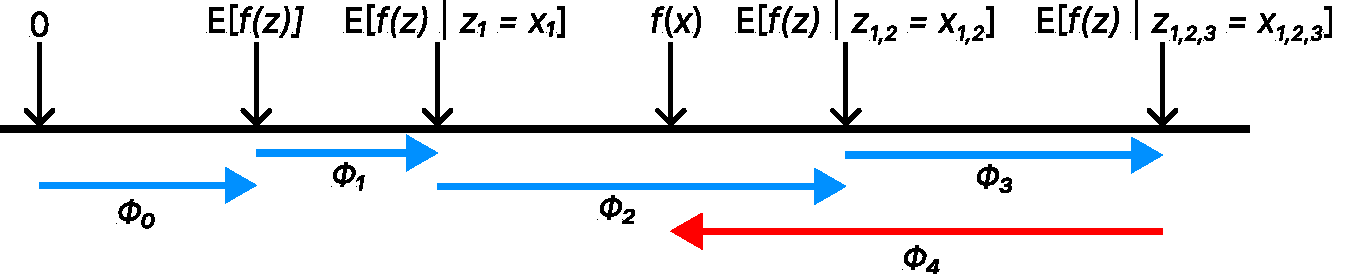
\includegraphics{obrazky-figures/shap/theory/shap_values.pdf}
		}
		\caption{Grafový příklad výpočtu hodnoty SHAP}
		\label{fig:SHAP_values}
\end{figure}

% SHAP limits
\subsubsection{Omezení} \label{subsubsec:SHAP_limits} 
Ačkoliv se jedná o~velmi prospěšnou metodu pro porozumění důležitosti příznaků a~jejich roli v~samotném modelu, má i~tato metoda svá omezení. Tím je myšlen zejména výpočetní čas, který se s~přibývajícími příznaky zvyšuje, a~to faktoriální časovou složitostí. V~menším počtu je tato metoda velmi přínosná, avšak s~větší škálou je nemožná~\cite{Shapley_limits}.

% SHAP graph single prediction
\subsubsection{Grafické zobrazení -- jedno pozorování} \label{subsubsec:SHAP_graphs_single_prediction} 
Jedná se o~grafy, které zobrazují jen pohled na jednu predikci, tudíž na nich lze vidět, jak zapůsobily jednotlivé příznaky a~jakou silou.

Je možné mezi ně zařadit například tzv. \texttt{force plot}. Na obrázku~\ref{fig:SHAP_force} je znázorněna jedna predikce, která byla vyhodnocena jako malware, což je vidět negativní hodnotou na dané ose. Červeně znázorněné příznaky a~jejich hodnoty posouvají výslednou hodnotu do vyšších hodnot, naopak modré hodnoty níže. Jejich výsledná hodnota pak rozhodne, zda se jednalo o~benigní či malware doménu.
\begin{figure}[H]
    \centering
		\scalebox{0.4}{
			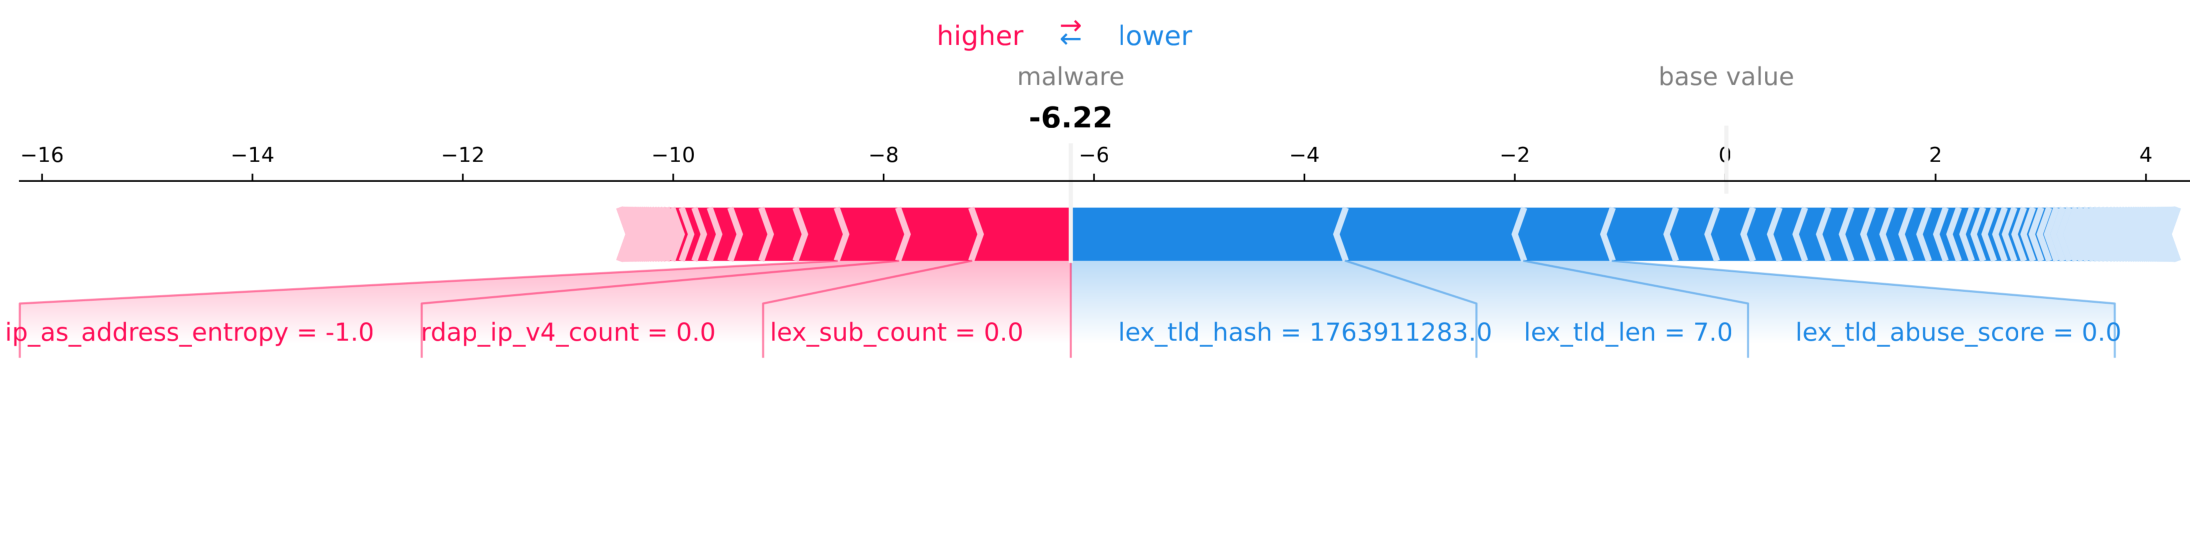
\includegraphics{obrazky-figures/shap/theory/shap_force_xgb_malware.pdf}
		}
		\caption{Příklad zobrazení grafu SHAP force plot}
		\label{fig:SHAP_force}
\end{figure}

Dalším typem tohoto druhu grafů je tzv. \texttt{waterfall plot}, který funguje na stejném principu jako již zmíněný \texttt{force plot}, viz obrázek~\ref{fig:SHAP_force}. Jedinou odlišností je vzhled tohoto grafu, díky čemuž je možno vyčíst další údaje o~příznacích. U~tohoto typu grafu je možné vidět, který příznak má největší účinek a~jsou zde právě seřazené dle účinnosti. Barvy fungují na stejném principu, kdy červená barva posouvá predikci do kladných hodnot a~modrá naopak do záporných. Stejnou predikci pro srovnání, co mohou ukazovat dané grafy, jako na obrázku~\ref{fig:SHAP_force} můžeme tedy vidět i~na obrázku~\ref{fig:SHAP_waterfall}, kde však byl použit vodopádový typ.

\begin{figure}[H]
    \centering
		\scalebox{0.47}{
			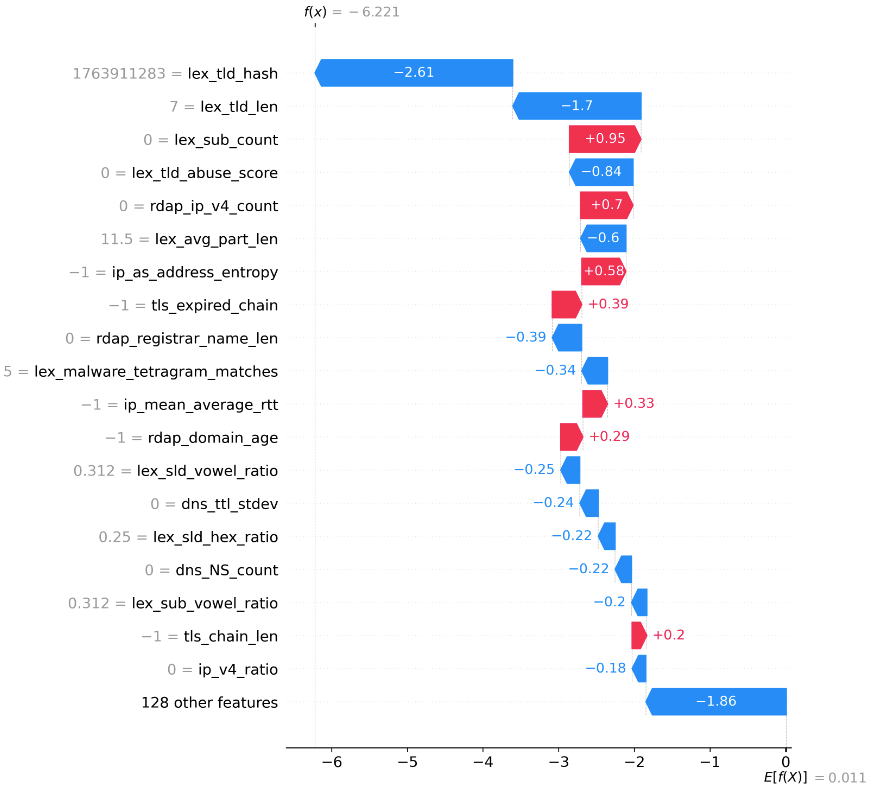
\includegraphics{obrazky-figures/shap/theory/shap_waterfall_xgb_malware.png}
		}
		\caption{Příklad zobrazení grafu SHAP waterfall plot}
		\label{fig:SHAP_waterfall}
\end{figure}

% SHAP graph summary
\subsubsection{Grafické zobrazení -- celkový pohled} \label{subsubsec:SHAP_graphs_summary} 
Tyto grafy je možné implementovat pomocí funkce \uv{summary plot} s~přesnějšími parametry po změnu vzhledu, typu grafu atd. Díky těmto grafům je možné získat průměrný dopad jednotlivých příznaků na určování. Ať už se jedná o~\texttt{bar plot}, který nám pouze ukazuje váhu jednotlivých příznaků nehledě na jejich pozitivní či negativní účinek, nebo o~\texttt{dot plot}, který zobrazuje právě zmíněný vliv, zda pomáhá při detekci pozitivně, tudíž pro benigní část, nebo negativní malware část.

Souhrn průměrných hodnot \Gls{SHAP}, které byly spočítány pro každý příznak zvlášť, je možné vidět na obrázku~\ref{fig:SHAP_bar}, což je graf v~režimu \texttt{bar plot}, kde je znázorněno 5 nejvlivnějších příznaků při rozhodování, zda je doména špatná či nikoliv. Bere se zde její absolutní hodnota, takže v~tomto grafu nezjistíme, zda-li je více prospěšná pro benigní domény, či pro malware. Na ose x~je možné vidět absolutní průměrné hodnoty, kterých daná hodnota příznaku dosahuje, a~na ose y~jsou názvy daných příznaků.
\begin{figure}[H]
    \centering
		\scalebox{0.59}{
			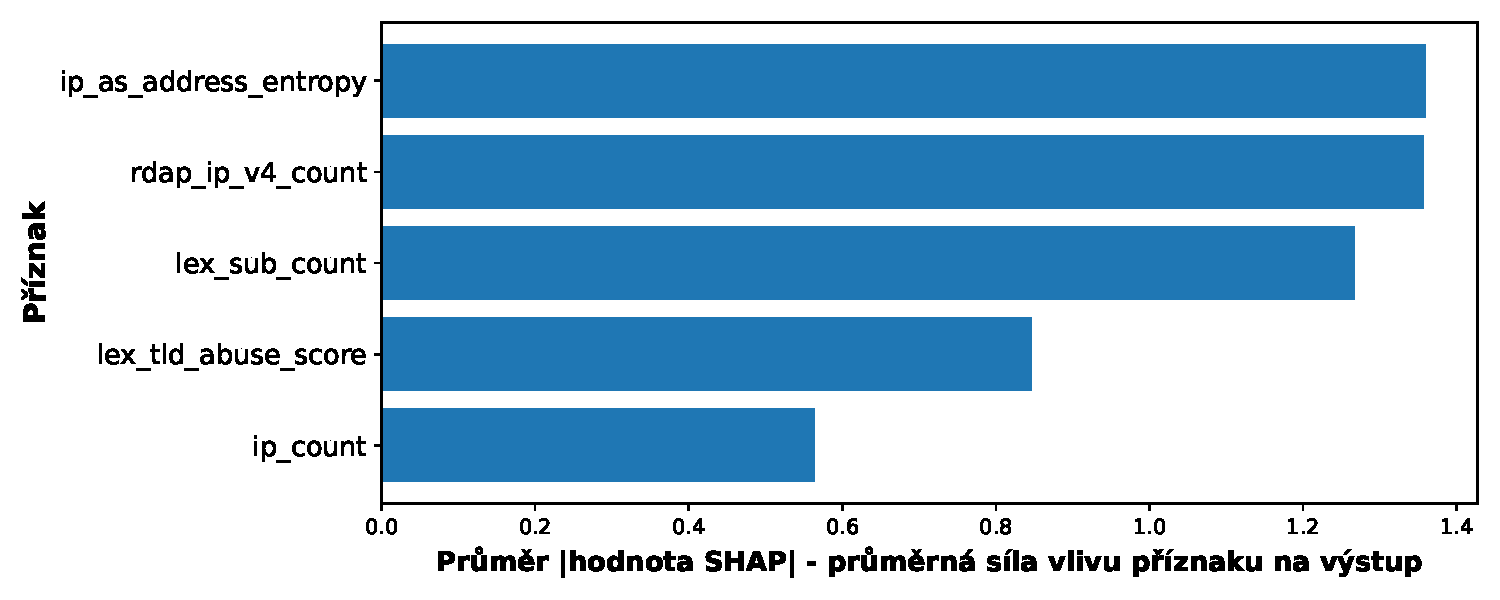
\includegraphics{obrazky-figures/shap/theory/shap_top5_bar_xgb_malware.pdf}
		}
		\caption{Příklad zobrazení grafu SHAP summary plot v~jeho typu zobrazení \texttt{bar}}
		\label{fig:SHAP_bar}
\end{figure}

Vliv jednotlivých příznaků je možné pozorovat i~v~jiném režimu souhrnných grafů. Na obrázku~\ref{fig:SHAP_dot}, což je graf v~režimu \texttt{dot plot}, je možné získat i~negativní hodnoty, takže je možné lépe zkoumat vliv daného příznaku vzhledem k~typu. Některé příznaky totiž mohou fungovat zejména pozitivním způsobem a~rozhodovat nejvíce pro pozitivní část výsledku. Na grafu se nacházejí hodnoty \Gls{SHAP} na ose x, kdy negativní část odpovídá malware, kladná naopak benigním. Na ose y~jsou jednotlivé příznaky a~samotná barva pak určitě danou hodnotu příznaku.
\begin{figure}[H]
    \centering
		\scalebox{0.59}{
			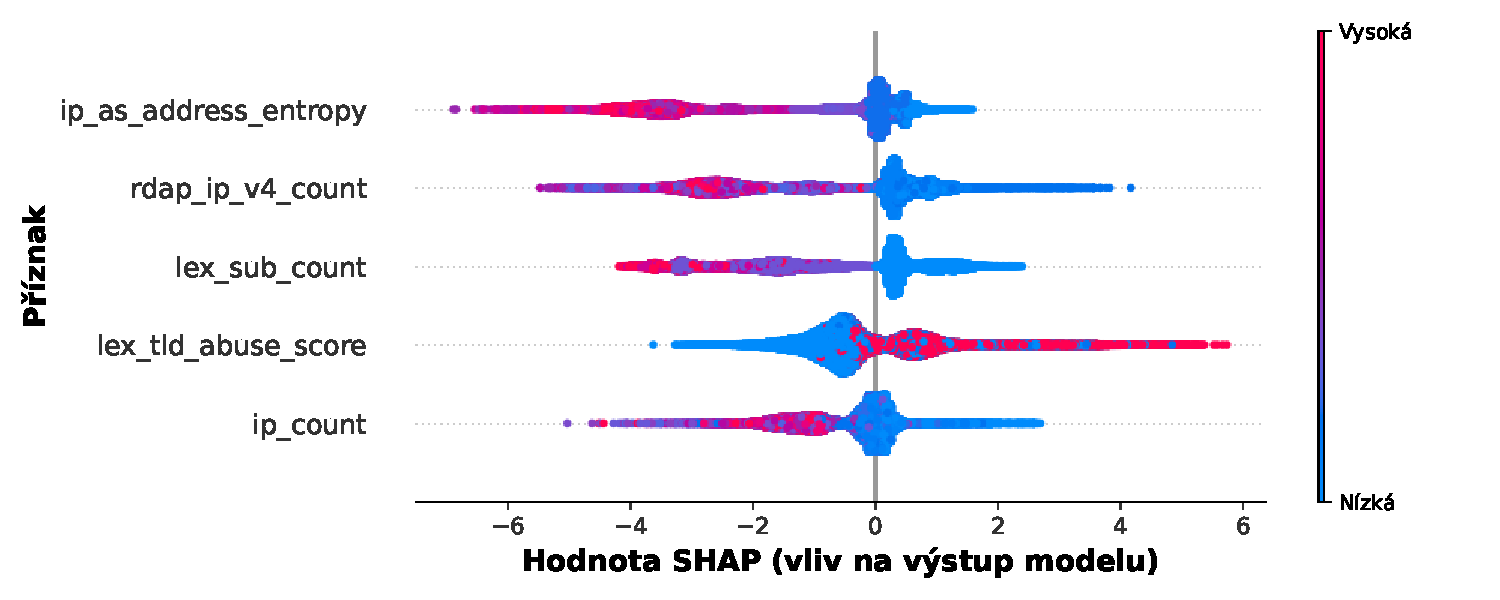
\includegraphics{obrazky-figures/shap/theory/shap_top5_dot_xgb_malware.pdf}
		}
		\caption{Příklad zobrazení grafu SHAP summary plot v~jeho typu zobrazení \texttt{dot}}
		\label{fig:SHAP_dot}
\end{figure}

% Hyperparameter tuning
\section{Vylepšování hyperparametrů} \label{sec:Hyperparameter_tuning}
Nastavení a~postupné vylepšování hyperparametrů jsou klíčové kroky při samotném vývoji modelů. Tyto parametry se neučí z~dat, ale jsou nastavené ještě před samotným začátkem trénování. Díky nim je možné významně ovlivňovat výkon daného modelu, ale zároveň jejich optimální nalezení může být mnohdy obtížné, zejména časově.
Existuje několik způsobů hledání nejoptimálnějších parametrů. Mezi ně můžeme zařadit například následující zmíněné.

% Grid Search
\subsubsection{Grid Search} \label{subsubsec:GridSearch}
Je to jednoduchý a~zároveň jeden z~nejrozšířenějších způsobů na hledání nejoptimálnějších hyperparametrů pro co nejlepší výkonnost modelu, ale může být velmi zdlouhavý vzhledem k~počtu hledaných hyperparametrů. Zahrnuje definici rozsahů hodnot pro každý hyperparametr a~poté testování všech kombinací. Je snadno implementovatelný, ale s~přibývajícím počtem dimenzí se stává výpočetně náročným.

Nejdříve je potřeba definovat samotný Grid Search a~to pomocí předání modelu, metriky pro měření výkonnosti (například přesnost), počtu testování při dané kombinaci a~v~neposlední řade taky námi definované slovníky hyperparametrů, které chceme testovat. 

Po otestování všech možných kombinací můžeme pomocí \verb|best_estimator_| zjistit model s~nejlepší sadou hyperparametrů, díky \verb|best_params_| zjistíme samostatnou sadu. Další možností je i~získání nejlepšího skóre skrz \verb|best_score_|, které bylo dosaženo nejlepším modelem. Kód, význam parametrů a~pro celkového pochopení této metody jsem čerpal z~\cite{scikit-learn-GridSearchCV}.

% Random Search
\subsubsection{Random Search} \label{subsubsec:RandomSearch} 
Řadí se mezi další možné způsoby, kdy může být velmi efektivní alternativou k~již předchozímu zmíněnému Grid Search, viz \ref{subsubsec:GridSearch}. Výhodou je, že může najít rychleji dobré hyperparametry, protože z~dané množiny vybírá kombinace náhodně. 

Samotná implementace tohoto způsobu je velmi podobná až na přidání počtu opakování náhodného vybírání kombinací. Výsledky pak získáme stejným způsobem, jako u~Grid Search. Kód, význam parametrů a~pro celkového pochopení této metody jsem čerpal z~\cite{scikit-learn-RandomSearch}.

\subsubsection{Bayesian Search}
Bayesovské vyhledávání ve strojovém učení se vztahuje k~bayesovské optimalizaci hyperparametrů, což je technika používaná k~nalezení nejlepšího nastavení hyperparametrů modelu strojového učení. Na rozdíl od tradičních metod, jako je Random Search nebo Grid Search, využívá bayesovská optimalizace výsledky předchozích vyhodnocení k~systematickému zpřesňování parametrů a~zaměřuje se na kombinace, které s~největší pravděpodobností přinesou lepší výkon. Kód, význam parametrů a~pro celkového pochopení této metody jsem čerpal z~\cite{scikit-learn-BayesSearch}.


%-----------------------------------------------------
% Collect and save data
\chapter{Sběr a~ukládání dat} \label{chap:Collect_and_save_data}
Prvním blokem celé funkčnosti je samotný sběr a~uložení datové sady, která je poté využita pro trénování modelu. V~sekci~\ref{sec:Load_domains} je blíže vysvětleno z~jakých zdrojů získávám malware domény a~následně jak probíhá jejich samotné ověření, zda jsou opravdu škodlivé v~sekci~\ref{sec:Verification_malware}. Poslední částí této sekce je jak probíhá samotný sběr pomocí získávání z~dostupných externích informací a~jejich ukládání v~sekcích~\ref{sec:Collecting}~a~\ref{sec:Saving_data}.

Na obrázku~\ref{fig:schema} je možné vidět detailní zpracování celého postup od sběru dat až po finální natrénování výsledného modelu. Podrobněji jsou jednotlivé části rozebrány v~následujících kapitolách a~jejich sekcích.
\begin{figure}[H]
    \centering
		\scalebox{0.28}{
			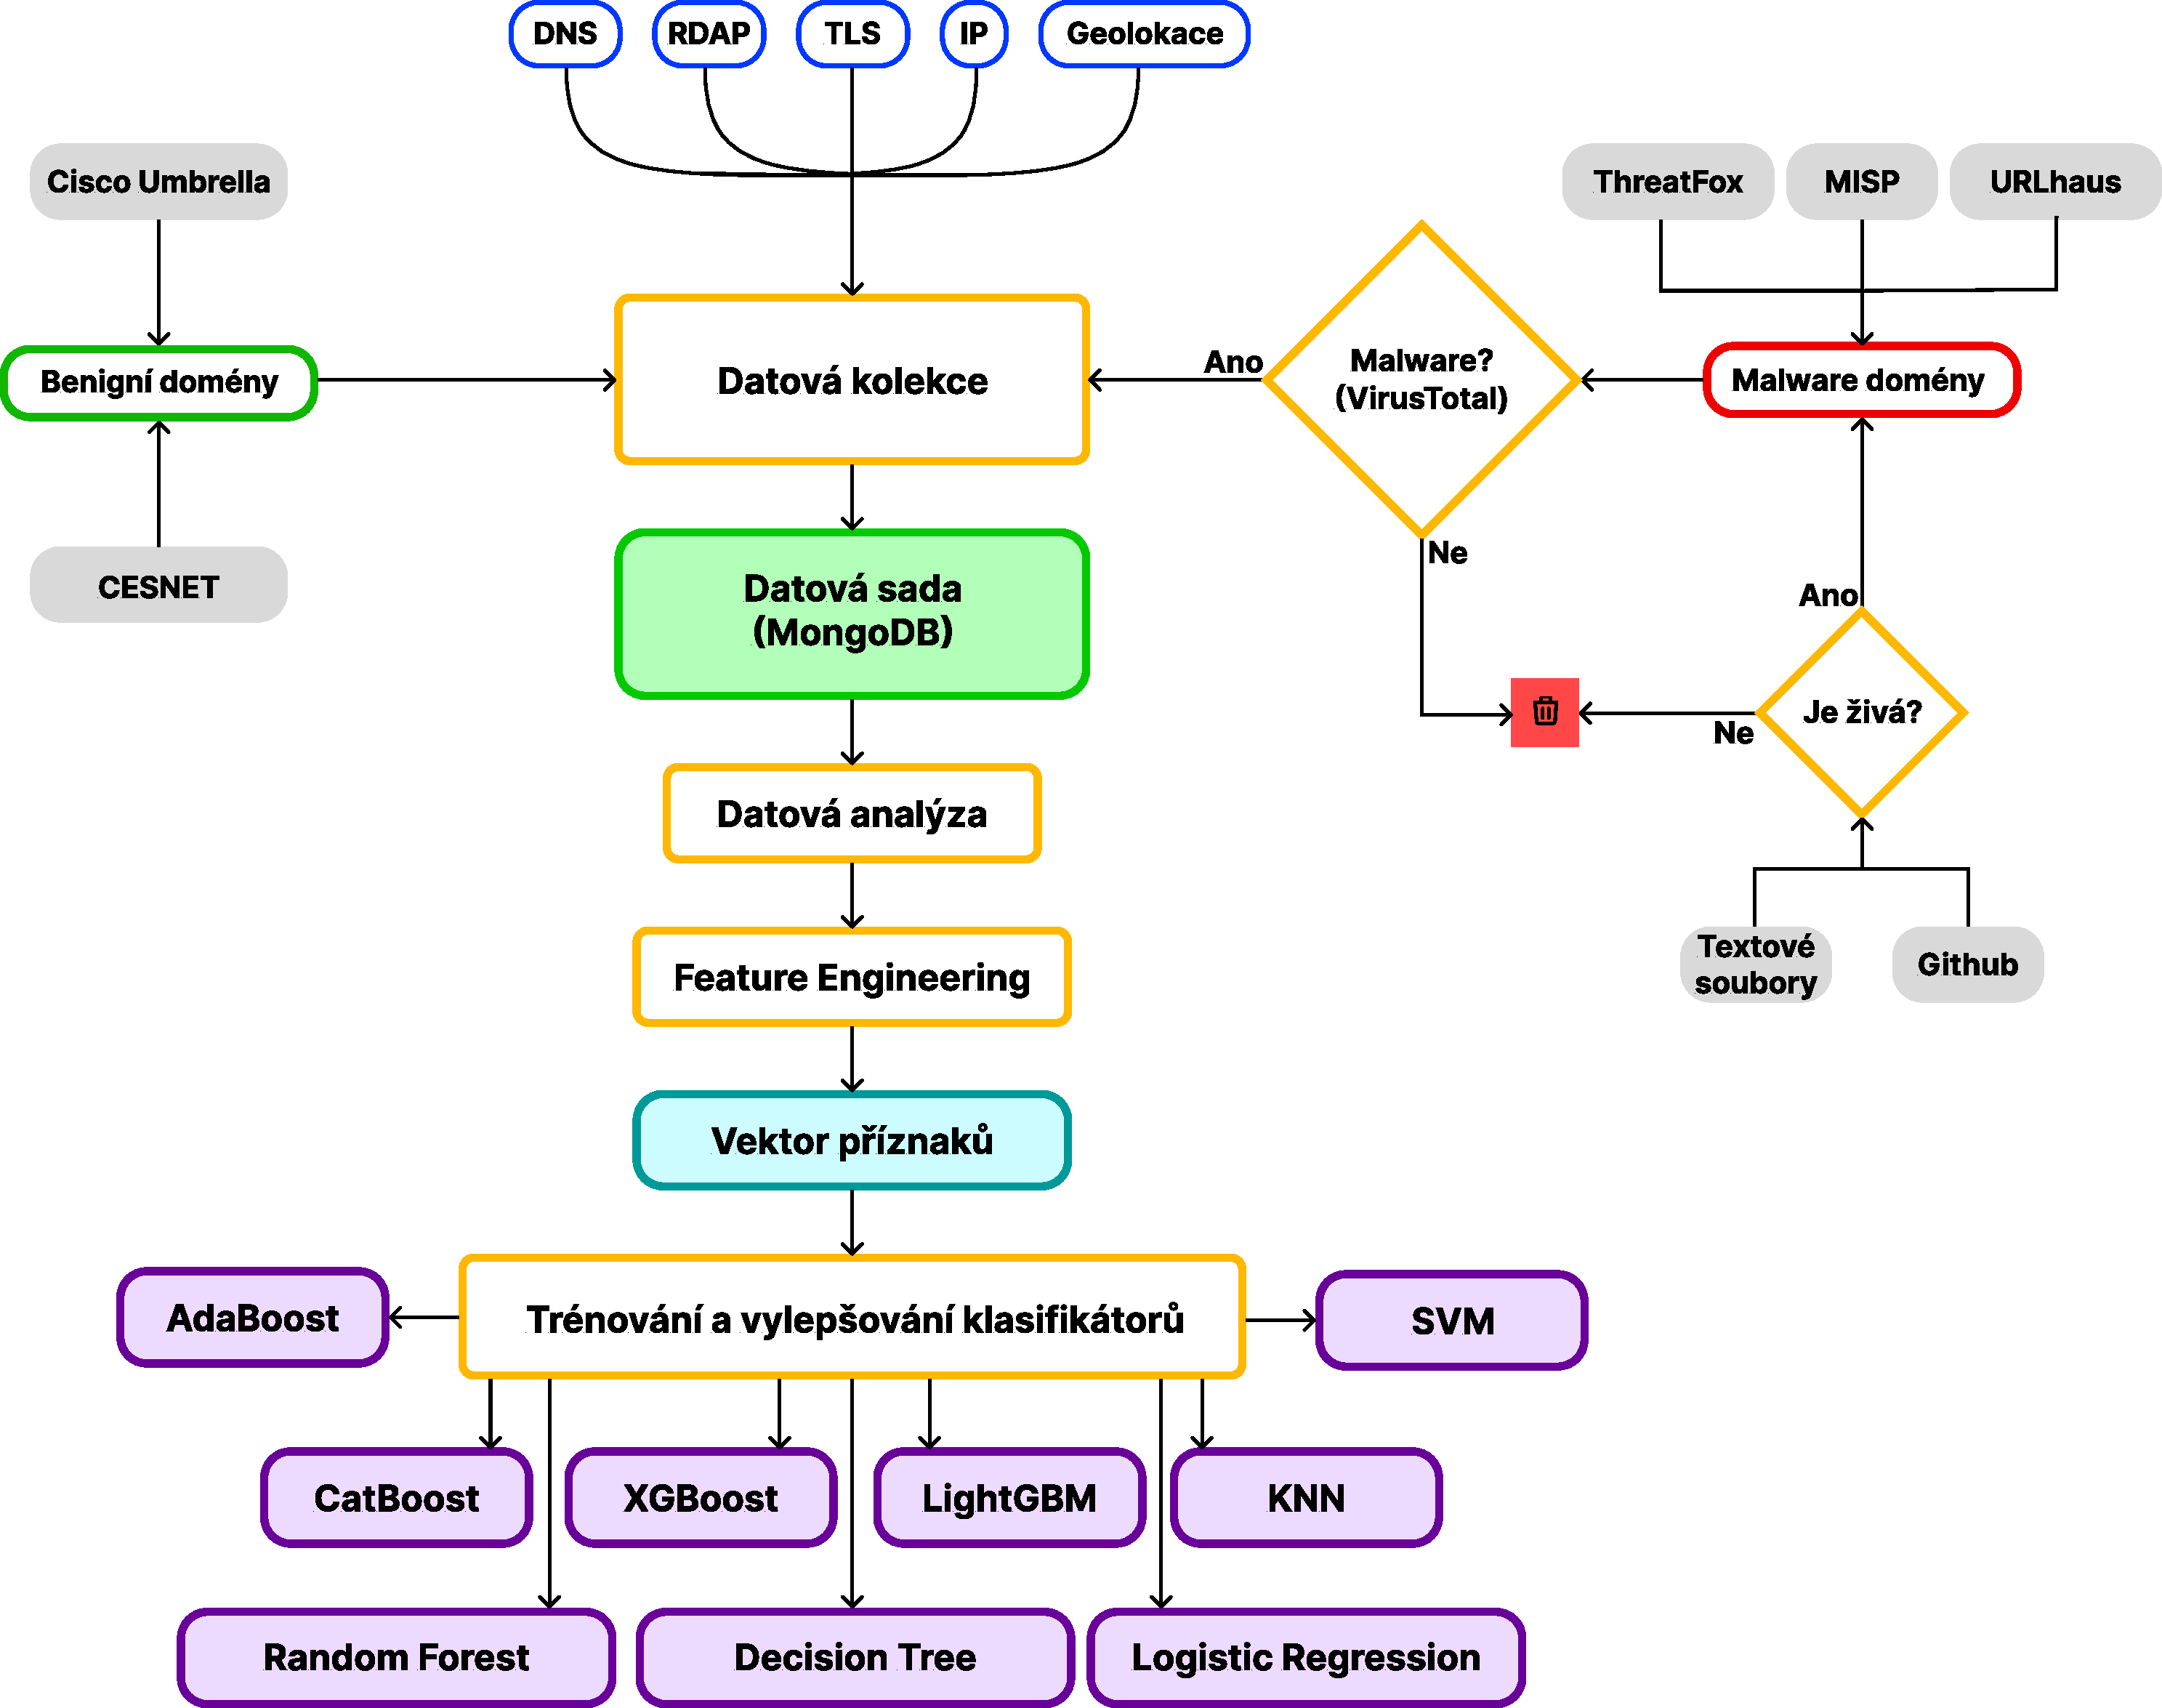
\includegraphics{obrazky-figures/schema.pdf}
		}
		\caption{Schéma návrhu implementace}
		\label{fig:schema}
\end{figure}

% Load domains
\section{Získávání domén} \label{sec:Load_domains}
Benigní, neboli také jinak řečeno nezávadné, domény jsem získal z~Cisco Umbrella a~od sdružení CESNET. Tento tým algoritmem v~průběhu času získával domény, které jsou nejpoužívanější a~je u~nich ověřená nezávadnost. Tato část datové sady je získána z~průběhu delšího časového období, kdy se využívaly zejména domény, které se objevují v~tomto seznamu nejčastěji.

Do maligní, v~mém případě malware části sady jsem získával domény z~různých zdrojů. Mezi hlavní zdroje je možné zařadit ověřené stránky, které každý den přidávají stovky těchto domén veřejně a~je možno přes jejich rozhraní tato data průběžně získávat. Je možné zde zařadit zejména ThreatFox\footnote{ThreatFox -- \url{https://threatfox.abuse.ch/}} (40 206 domén), kde lze i~dohledat o~jakých typ malwaru se jedná, viz přílohu~\ref{fig:malware_types}, MISP\footnote{MISP Threat Sharing -- \url{https://www.misp-project.org/}} (7 845 domén) a~URLhaus\footnote{URLhaus -- \url{https://urlhaus.abuse.ch/}} (4 013 domén), kdy denně bylo možné získat z~těchto zdrojů dohromady přibližně 500 domén. Po čase se mi povedlo najít stránku Rescure\footnote{Rescure -- \url{https://rescure.me/}} (2 781 domén), ze které jsem získával průměrně 400 domén za den.\\
Bohužel počet získaných domén v~kratším časovém období jen z~těchto zdrojů by byl nedostačující a~proto jsem vyhledával i~různá fóra, stránky nebo dokumenty obsahující lidmi sesbírané domény, mezi které je možné zařadit The Firebog (17 793 domén)~\cite{Firebog, Firebog2}, Spam404 (1 853 domén)~\cite{Spam404}, Steven Black (35 199 domén)~\cite{StevenBlack} a~další blacklisty z~GitHubových účtů (21 236 domén)~\cite{AssoEchap, DandelionSprout, maravento, stamparm, ethanr, quidsup}. Často tyto seznamy obsahovaly až deseti tisíce domén. Díky nim se datová sada rozrostla, což přispívá k~možnosti lépe trénovat daný model.

Mým přínosem tudíž bylo nejen prozkoumání různých možných použitelných zdrojů, kde by se mohly nacházet kvalitní seznamy malware domén, ale i~díky nim jsem původní datovou sadu, která mi byla dostupná už od počátku práce, rozšířil z~původních 46 tisíc na 131 tisíc domén. Toto číslo by se ještě zvětšilo, pokud bych bral i~mrtvé nebo neprofiltrované domény, ale snahou je získat co nejkvalitnější data, tudíž jsem se raději rozhodl pro nižší počet, ale za to kvalitnější. 

% Verification of malware domains
\section{Ověřování domén} \label{sec:Verification_malware}
Aby získané informace k~dané doméně byly kompletní nebo aspoň co nejvíce obsažené, je potřeba, aby doména byla aktivní. Proto zvláště u~těch, které byly získané z~fór nebo textových souborů sdílených lidmi, je potřeba vybírat jen ty, které jsou aktivní. Pomocí programu ping\footnote{PING -- Packet InterNet Groper} lze zjistit funkčnost spojení mezi námi a~danou doménou. Pokud nepřijde odpověď, považuji tuto doménu za neaktivní a~následně jsem ji odebral ze seznamu, protože by mi poskytovala pouze lexikální údaje.

Po omezení dat, které by neměly úplné informace, jsem musel zkontrolovat, zda je vůbec daná doména maligní a~především malware. K~této verifikaci jsem využíval program VirusTotal\footnote{VirusTotal -- \url{https://www.virustotal.com/}}, díky kterému je možno získat data od antivirů, které danou doménu prohlásily za škodlivou či nikoliv. Ve většině případech i~specifikují o~jaký typ nebezpečí se jedná, což pomáhá při rozhodování, zda-li danou doménu nechat v~datové sadě, abychom trénovali čistě malware. Tento přístup byl inspirován Petrem Poučem, který využil tento způsob již na validaci phishingových domén, tudíž se dalo lehce upravit tento přístup na malware domény. Toto řešení se ukázalo jako funkční a~použitelné, neboť díky tomuto bylo vyřazeno větší množství domén, které by svojí neškodností nakonec uškodili výslednému trénování.

% Collecting
\section{Sběr} \label{sec:Collecting}
Samotný sběr je prováděn pomocí programu\footnote{dr-collector -- \url{https://github.com/oviOvocny/dr-collector/}} od Ing. Adama Horáka~\cite{Horak2023thesis}, který je postupně vyvíjen i~dalšími pracovníky. Využití tohoto programu bylo rozhodnutí pro co nejlepší kompatibilitu daných datových sad získaných již z~dřívějších měsíců jak v~benigních, tak i~v~malware doménách. Zejména preciznost a~vhodný způsob ukládání v~JSON formátu je tato forma sběru ideální pro mou práci. 

Po mé úpravě jsem byl schopný načíst nové domény z~již zmíněných zdrojů a~automaticky k~nim dosbírat všechny potřebné informace. Případně tento sběr informací provést vícekrát, aby bylo nasbíráno vše, co je možné.

% Saving data
\section{Ukládání dat} \label{sec:Saving_data}
Pro ukládání datové sady jsem zvolil databázi MongoDB\footnote{MongoDB -- \url{https://www.mongodb.com/}} a~to zejména díky její možnosti snadné a~efektivní práce se strukturovanými daty. Díky tomu, že se jedná o~noSQL databázi, nemá předem definované kompletní schéma a~tudíž se dá struktura během práce měnit. Je zde možné taky pracovat jednotným způsobem s~více typy dat a~o~různé struktuře, což je pro moji práci velmi příhodné. Tuto 
databázi jsem pustil ve vlastním Docker\footnote{Docker -- \url{https://www.docker.com/}} kontejneru pro lepší zabezpečení a~přívětivost obsluhy. Při každém sběru je spuštěn kontejner, nasbírána data a~poté vypnut, aby k~němu nebyl přístup z~jiných zdrojů. Průběžně jsem také dělal zálohy těchto sad, kdyby náhodou přišel nějaký nežádaný útok na tuto databázi. 

% MongoDB
\subsubsection{MongoDB} \label{subsubsec:MongoDB}
Jedná se multiplatformní dokumentovou databázi. Řadí se mezi noSQL databáze a~využívá místo tabulek dokumenty podobné formátu JSON, přesněji BSON (binární JSON). Ty jsou pak shromážděny do dané kolekce, kdy jedna databáze může obsahovat více kolekcí. Využívá dynamické databázové schéma, které umožňuje rychlejší a~jednodušší vytváření a~integraci dat~\cite{MongoDB}.

% Docker
\subsubsection{Docker} \label{subsubsec:Docker}
Celou databázi jsem oddělil do vlastního Docker kontejneru, což je izolované prostředí, které má v~sobě všechny závislosti pro fungování daného programu. Obraz kontejneru Docker je lehký, samostatně spustitelný balíček softwaru, který obsahuje vše potřebné ke spuštění aplikace: kód, běhové prostředí, systémové nástroje, systémové knihovny a~nastavení~\cite{Docker}. Tento přístup byl vybrán zejména v~rychlosti spuštění daného kontejneru oproti virtuálním strojům.


%-----------------------------------------------------
% Feature engineering
\chapter{Feature Engineering} \label{chap:Feature_engineering}
Ještě před samostatným trénováním klasifikátorů je nutné vybrat, na jakých příznacích se bude klasifikátor trénovat a~rozhodovat. K~tomu je potřeba definice příznaků založených na zjištění zajímavých vlastností v~datech, k~čemuž mi posloužila datová analýza, která je podrobněji rozepsána v~sekci~\ref{sec:data_analyzation}, ze které pak mohl vzniknout finální vektor příznaků, o~kterém je více slov v~sekci~\ref{sec:feature_vector}.

\section{Datová analýza} \label{sec:data_analyzation}
Pro lepší pochopení, co je pro malware domény unikátní a~jakými rysy se liší od těch benigních, je potřeba provést datovou analýzu. Ta nám pomůže nejen s~tímto pochopením, ale i~k~vytvoření příznaků, na základě kterých pak samotný klasifikátor může trénovat a~detekovat domény.

\subsection{Lexikální analýza doménových jmen}
Jako první jsem prozkoumal domény první úrovně, neboli \texttt{top-level domains} (\Gls{TLD}). U~nich jsem zjistil, že oba typy domén mají jako nejčastější typ \texttt{.com}, což odpovídá, neboť je to nejčastější používané \Gls{TLD}~\cite{Bianchi_2023}. U~malware domén toto zastoupení dosahovalo 50~\%, ale i~u~benigních se vyskytovala nejčastěji, přesněji kolem 38~\%. Poslední podobnost měly v~zastoupení \texttt{.net} domény. V~dalších částech se už začaly lišit, kdy u~benigních se nejčastěji vyskytovaly státní domény a~nebo \texttt{.org}, naopak u~malware převažovaly domény jako například \texttt{xyz, site, top}, ale také například domény z~Ruska. Ale všechny tyto typy už nepřesáhly zastoupení větší než 5~\%.

Jako další jsem zkoumal doménové jméno jako celek. Převážně jsem se zaměřoval na výskyt jednotlivých charakterů, díky čemuž jsem zjistil, že malware domény mají průměrně více písmen v~doménovém jméně než benigní domény. S~počtem číslic, speciálních znaků a~hexadecimálních znaků už byly na tom shodně. Naopak v~průměrné délce se jevily benigní domény jako delší, kdy ale pokud bychom vzali zase jen části domén, tak zde mají malware domény průměrně nejdelší část domény, což se poté reflektuje i~na celkové průměrné délce části doménového jména. To je však nejspíše způsobeno i~tím, že benigní domény mají v~průměru více poddomén než malware domény. 

\subsection{Analýza dat z~DNS záznamů}
Díky inspiraci výzkumnou skupinou FETA jsem více prozkoumal data, která šla získat z~\Gls{DNS} záznamů. Méně než 2~\% malware domén má 3 a~více záznamů A, naopak nejčastější je 1 záznam, který se svým zastoupením blížil 45~\%. U~benigní části výskyty byly pravděpodobnější a~dosahovaly až 8 záznamů A, kdy nejvíce také bylo právě 1 záznamu A. Záznamy typu AAAA byly u~obou velmi podobné, kdy přes 80~\% obou částí neobsahovalo tento záznam. U~záznamů TXT a~MX velkých hodnot dosahovaly benigní doménová jména, kdy u~TXT dosahovaly hodnoty až 8 záznamům, u~malware bylo maximum 3 s~velmi malým zastoupením. Jedinou změnou byl záznam NS, kde malware domény převyšovaly a~objevují se častěji než u~benigních. Vše je vyobrazené na obrázku~\ref{fig:DNS_records}.

\begin{figure}[H]
    \centering
		\scalebox{0.42}{
                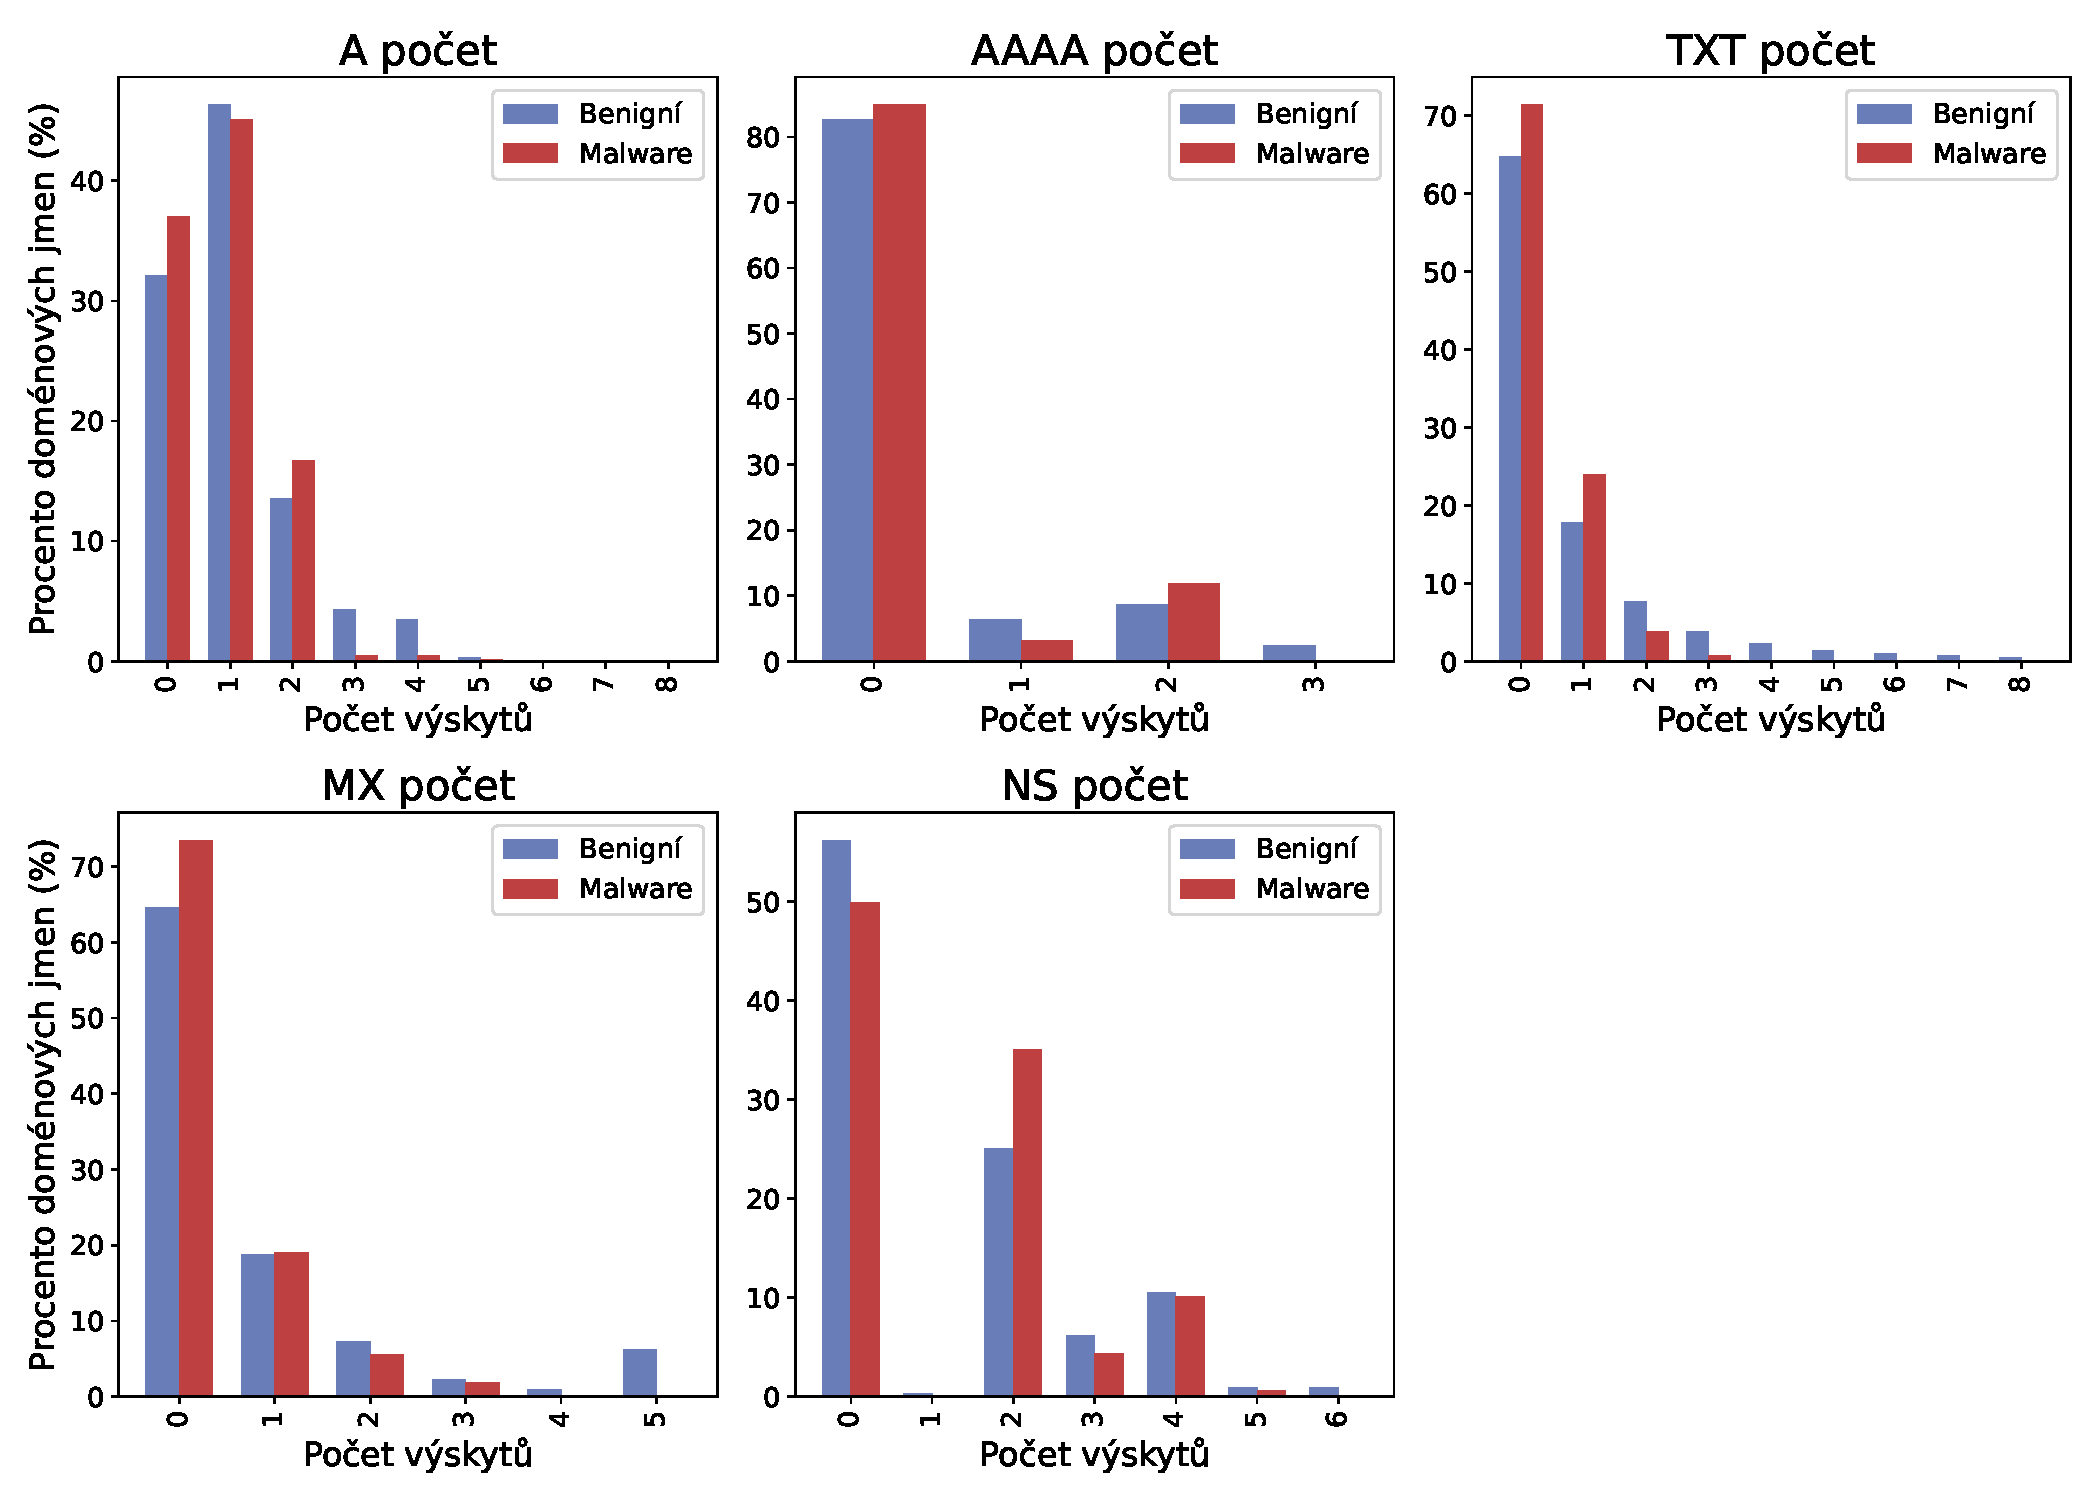
\includegraphics{obrazky-figures/analysis/DNS.pdf}
		}
		\caption{Počty záznamů v~DNS}
		\label{fig:DNS_records}
\end{figure}

\subsection{Analýza informací spojených s~IP adresami}
Pokud už malware doménová jména obsahovala IP adresy, tak se v~82~\% případech jednalo o~typ IPv4 typ adres. U~benigních toto číslo dosahovalo 72~\%, kdy zbytek patřil IPv6 adresám. Na tomto případě jde vidět, že zastoupení IPv6 adres není stále velkým trendem a~zvláště pro malware domény se zdá být zbytečné mít IPv6 adresu. 

Ačkoliv bych z~prvotních dat čekal, že počet IP adres (IPv4 i~IPv6) bude dosahovat značně vyšších hodnot u~benigních doménových jmen, tak u~obou typů domén se vyskytly i~doménová jména s~počtem IP adres větších než 25. Nejvíce dosahovaly u~benigních 31 adres, u~malware zase 29. Velké procento zastupovalo rozmezí 0 až 4 adres, což představovalo 84~\% z~celkového počtu adres u~benigních domén a~81~\% u~malware domén.

\subsection{Analýza dat získaných z~\Gls{RDAP}}
Na obrázcích~\ref{fig:RDAP_top10_benign} a~\ref{fig:RDAP_top10_malware} lze vidět zastoupení nejčastějších 8 registrátorů u~benigních a~malware domén. První pozici u~obou zastupuje \texttt{GoDaddy}, kdy u~benigních dat je o~trochu častěji. V~dalších už se začínají dosti lišit, kdy u~benigních převažuje ještě \texttt{MarkMonitor}, ale dále už si procenta rozdělují registrátoři celkem rovnoměrně. U~malware domén toto klesání zastoupení postupuje pomaleji, což jde vidět, neboť čtyři nejlepší mají zastoupení nad 5~\%. Mezi ně lze zařadit \texttt{NameCheap, eNom} a~\texttt{PublicDomainRegistry}. Z~rozboru životnosti jsem vypozoroval, že malware domény mají mnohem kratší životnost, mnohem častěji se registrují a~také se u~nich častěji mění záznamy v~\Gls{RDAP}. Získáním těchto hodnot jsem si jen potvrdil již dočtené tvrzení z~publikace~\cite{hason2020robust}.
\begin{figure}[H]
    \centering
		\scalebox{0.6}{
                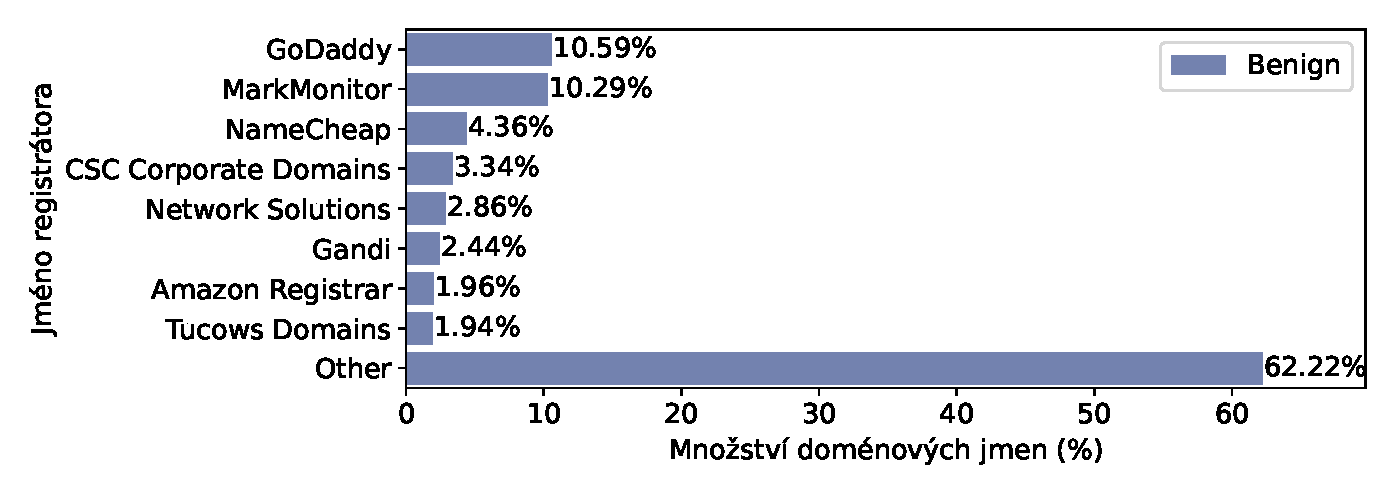
\includegraphics{obrazky-figures/analysis/RDAP_benign.pdf}
		}
		\caption{TOP 8 registrátorů u~benigních domén}
		\label{fig:RDAP_top10_benign}
\end{figure}
\begin{figure}[H]
    \centering
		\scalebox{0.6}{
                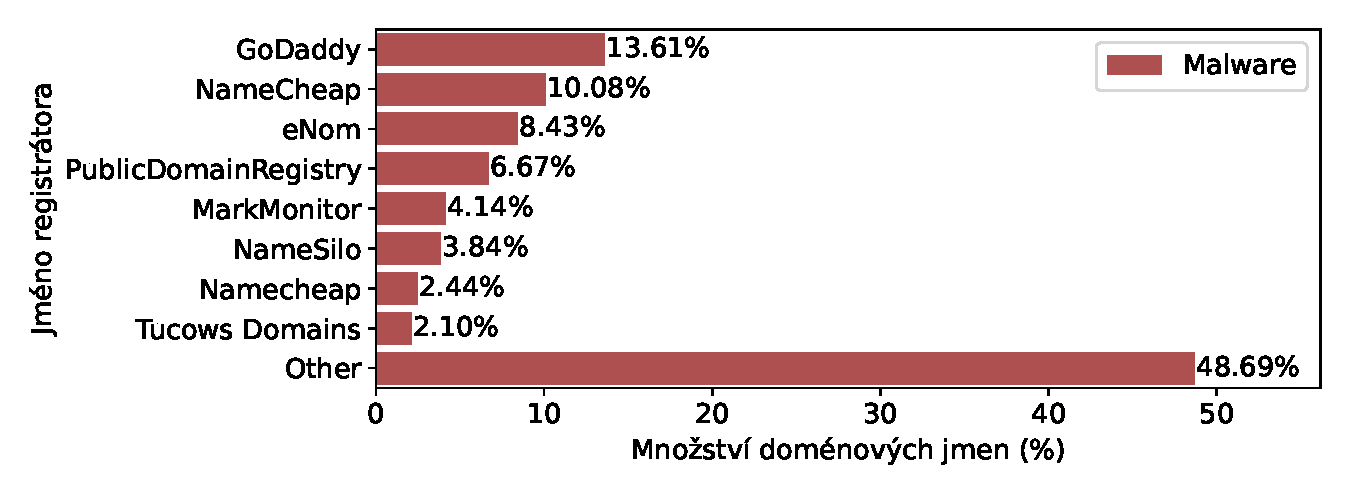
\includegraphics{obrazky-figures/analysis/RDAP_malware.pdf}
		}
		\caption{TOP 8 registrátorů u~malwarových domén}
		\label{fig:RDAP_top10_malware}
\end{figure}

\subsection{Analýza TLS certifikátů}
Pro domény s~dostupnými \Gls{TLS} daty (83.06~\% benigní, 60.21~\% malware) jsem provedl analýzu certifikačních řetězců. Pouze 0.54~\% benigních a~3.1~\% malwarových doménových jmen, která obsahují data z~\Gls{TLS}, používají certifikáty s~vlastním podpisem. Nejvíce řetězců mělo mezi dvěma a~čtyřmi certifikačními autoritami, neboli listový certifikát pro webovou stránku, 0-2 mezistupně a~kořenový certifikát. Nejčastěji však u~obou případů měly řetězce 3 certifikační autority. Bytí bez mezi stupňových certifikátů u~benigních doménových jmen bylo v~zastoupení 33.94~\%, u~malwarových doménových jmen 27.11~\%.

Mezi nejčastější listové certifikační autority benigních doménových jmen lze zařadit \texttt{Let's Encrypt} (18.63~\%), \texttt{Internet Security Research Group} (17.5~\%) a~\texttt{DigiCert Inc} (10.46~\%). U~malwarových doménových jmen se nejvíce objevovaly \texttt{Internet Security Research Group} (22.38~\%), \texttt{Let's Encrypt} (20.34~\%) a~\texttt{Digital Signature Trust Co.} (15.11~\%). Škodlivé domény využívají skupinu ISRG (Internet Security Research Group), protože ta provozuje certifikační autoritu Let's Encrypt, která vydává bezplatné certifikáty SSL/TLS se zjednodušeným procesem, díky čemuž může každý snadno zabezpečit své webové stránky.

\subsection{Analýza geolokačních údajů}
Poslední část datové analýzy jsou geolokační údaje, neboli na jakém místě na světě se daná IP adresa nachází. Proto jsem si pro tuto analýzu vyextrahoval souřadnice IP adres, kdy jsem poté zobrazil jen unikátní výskyty. Při pohledu na obrázek~\ref{fig:GEO_world} je možné vidět, že nejvíce IP adres se nachází v~Evropě a~v~USA. Maligní jsou na tom velmi podobně, kdy v~USA se vyskytují zejména v~okolí New Yorku a~Washingtonu. Pokud přiblížíme pohled jen na Evropu, což je možné vidět na obrázku~\ref{fig:GEO_Europe}, tak si můžeme povšimnout, že mezi ohnisko maligních domén je možné zařadit Nizozemsko, kde je velký počet IP adres přiřazených právě malware doménám. Poté už menší ohniska vznikaly ve městech jako například Londýn, Paříž nebo Düsseldorf v~Německu. Benigní domény, přesněji řečeno jejich IP adresy, už jsou rozmístěny celkem rovnoměrně s~větší kumulací ve střední Evropě, Itálii, Velké Británii, Nizozemsku a~Belgii.

\begin{figure}[H]
    \centering
		\scalebox{0.55}{
                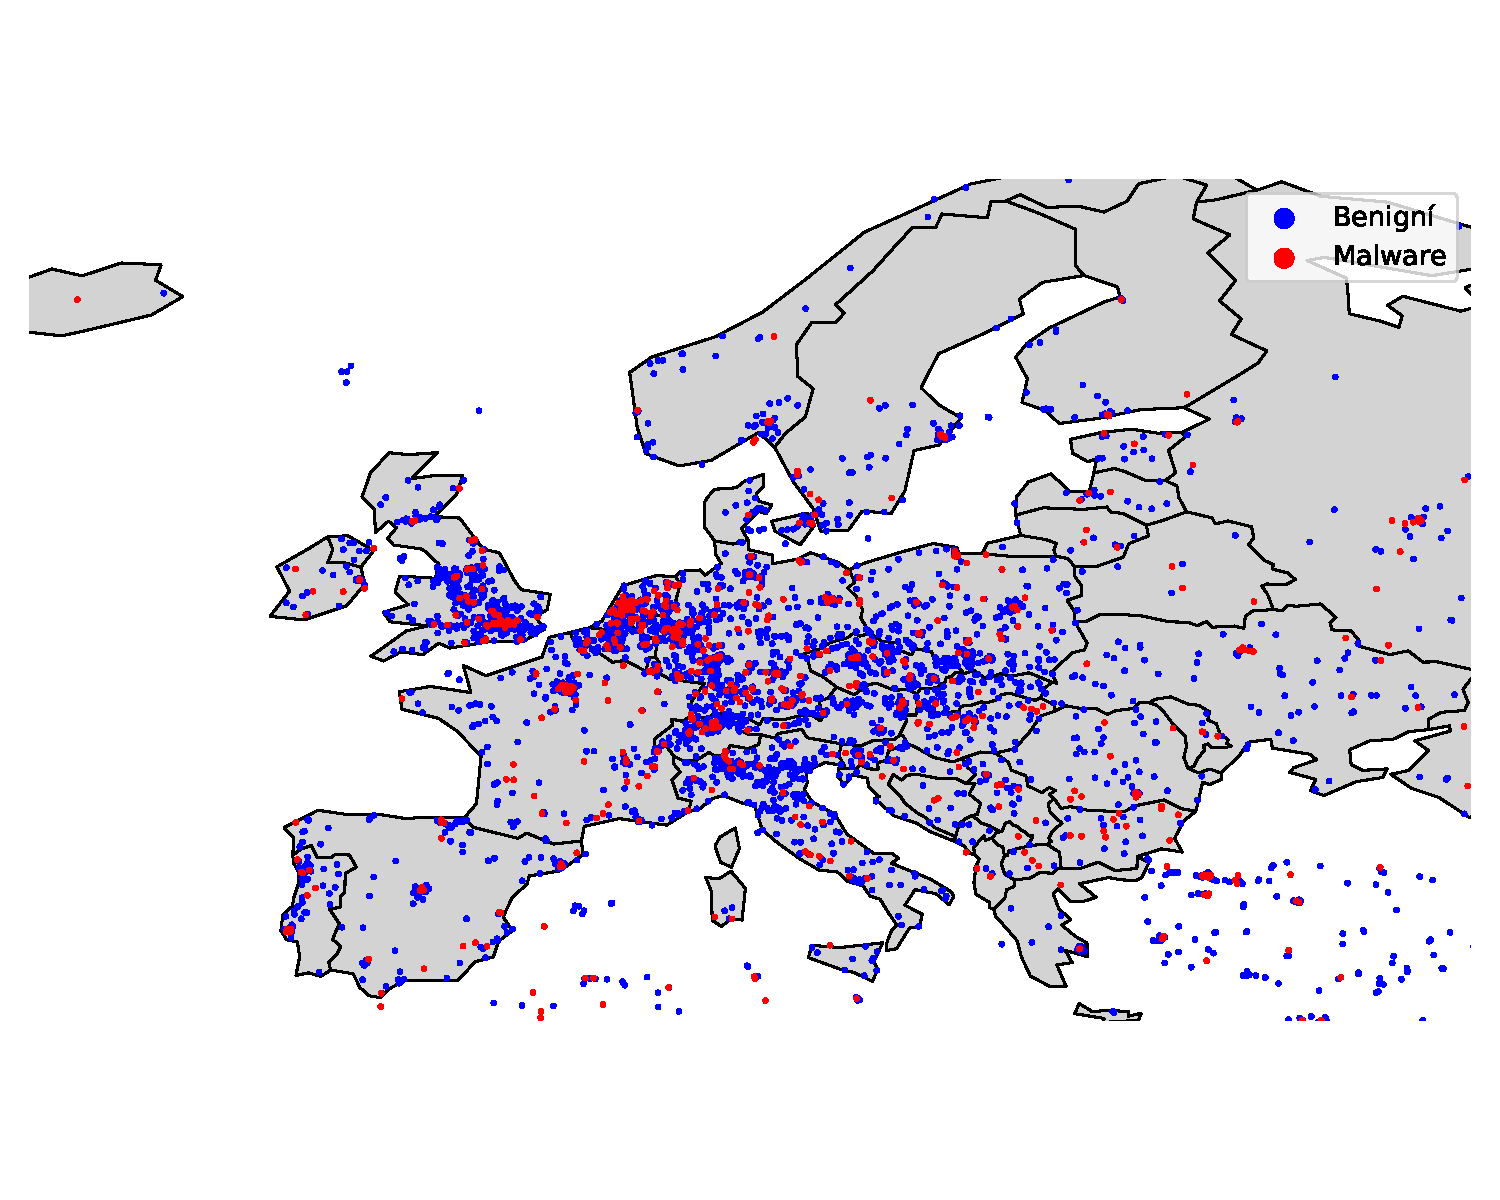
\includegraphics{obrazky-figures/analysis/GEO_Europe.pdf}
		}
		\caption{Bližší pohled na umístění IP adres v~Evropě}
		\label{fig:GEO_Europe}
\end{figure}

\begin{landscape}
    \begin{center}
        \begin{figure}[H]
            \centering
        		\scalebox{0.47}{
                        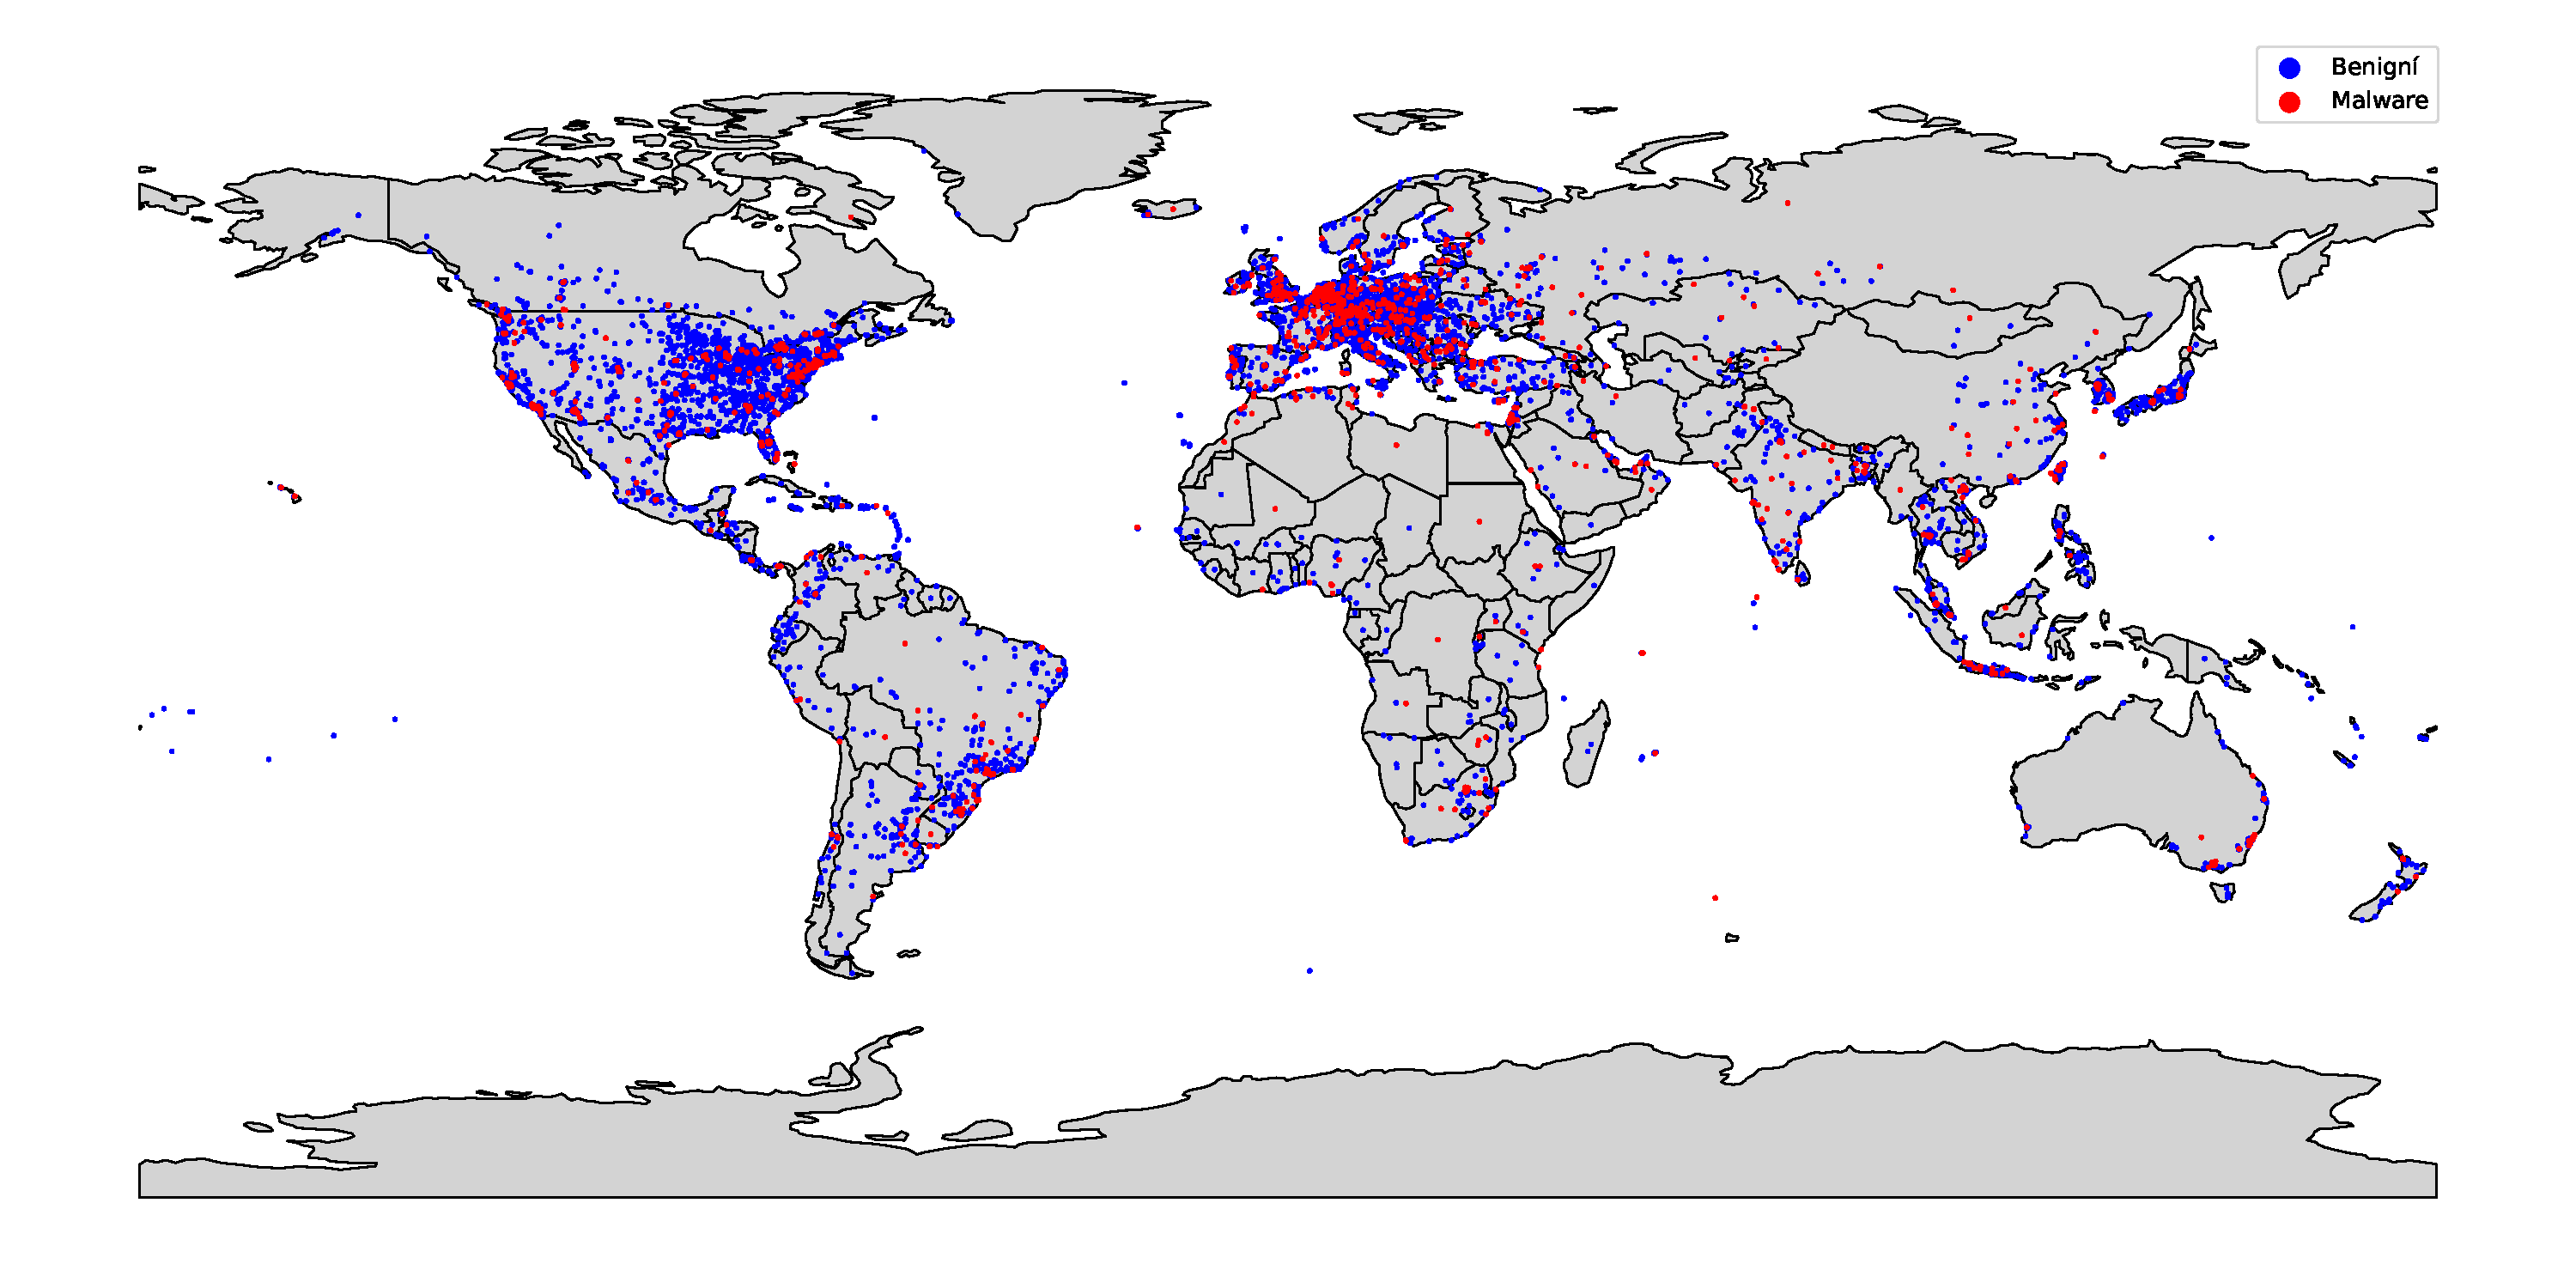
\includegraphics{obrazky-figures/analysis/GEO_world.pdf}
        		}
        		\caption{Umístění všech IP adres}
        		\label{fig:GEO_world}
        \end{figure}
    \end{center}
\end{landscape}


\section{Vektor příznaků} \label{sec:feature_vector}
Mnoho z~příznaků bylo inspirováno výzkumnou skupinou FETA a~odbornými pracemi, ale i~přes tuto skutečnost jsem musel provést datovou analýzu, abych ověřil, že tyto příznaky jsou vhodné pro moji detekci. Seznam všech použitých příznaků společně s~jejich přínosem spočítaném pomocí metody \Gls{SHAP} je možné vidět v~příloze~\ref{tab:all_features}.

Mezi první příznaky jsem zařadil ty, které slouží pro lexikální detekci, z~nichž některé, například délka doménového jména, jsou inspirovány z~práce~\cite{shi2018malicious}. Mezi další příznaky v~lexikální části jsem přidal i~n-gramy, které byly inspirací z~práce~\cite{10.1145/3465481.3465749}, což je vhodné pro detekci \Gls{DGA} domén. Také jsem mohl přidat například délku domény druhé úrovně, poměr jednotlivých znaků, počet souhlásek, ze kterých vznikly i~další příznaky na samohlásky, pomlčky, číslice a~jiné, což je potvrzeno pracemi~\cite{DBLP:journals/corr/WangS15d, 8560665}. Poté jsou lexikální příznaky, které jsou zaměřené na domény první úrovně (\textit{tld\_}), domény druhé úrovně (\textit{sld\_}) a~spojení všech poddomén (\textit{sub\_}). Mezi další je možné přidat, zda doménové jméno začíná číslicí nebo \uv{www}. S~inspirací výzkumnou skupinou FETA jsem přidal příznak, který reflektuje statisticky nejvíce zneužité domény první úrovně. Příznak \texttt{tld\_abuse\_score} je v~rozmezí od 0 do 0.6554 na základě dat získaných z~článku, který vydal Tim Adams~\cite{Adams_2021}.

Mezi celkový vektor příznak jsem přidal příznaky související s~\Gls{DNS}. Mezi základní příznaky lze brát počet a~obsah jednotlivých záznamů \Gls{DNS}, jak už zmínil ve svém výzkumu Kuyama a~spol.~\cite{kuyama2016method}. Díky výzkumné skupině FETA jsem přidal i~příznaky, které indikují, zda se v~záznamu TXT nachází SPF nebo DKIM, neboť zjistili, že se jedná o~přínosný příznak. 
\Gls{TTL}, což označuje dobu, po kterou může být \Gls{DNS} záznam uchován v~cache lokálního \Gls{DNS} serveru poskytovatele připojení k~internetu, jsem také přidal k~příznakům souvisejícím s~\Gls{DNS}. Tento typ příznaku byl inspirován zejména díky~\cite{shi2018malicious}, ale také skrz datovou analýzu, ve které jsem zjistil právě rozdílné hodnoty v~\Gls{TTL} záznamech.

Příznaky týkající se IP adres jsou odděleny zvlášť, i~když jsou získávány ze záznamů \Gls{DNS}. Mezi ně lze řadit celkový počet IP, IPv4, IPv6 adres, kdy jsem jejich rozdíly u~mých dvou testovaných tříd zaznamenal. Zahrnul jsme také průměrnou entropii IP prefixů, protože Perdisci a~kolektiv~\cite{6175908} naznačili, že nízká diverzita IP adres je často indikátorem škodlivých domén. V~neposlední řadě jsem zařadil s~ohledem na skupinu FETA i~průměrnou hodnotu RTT (Round Trip Time), což je doba mezi požadavkem na data a~jejich zobrazením.

Jako další jsem zařadil do vektoru i~příznaky týkající se hodnot z~\Gls{RDAP}u. Díky Kuyama a~kolektivu~\cite{kuyama2016method} jsem zjistil, že je možné zařadit informace o~registrátorech, žadatelích o~registraci a~administrativních kontaktech jako přínostné. Perioda registrace doménového jména, životnost domény, čas poslední změny byly inspirování ze studií~\cite{hason2020robust, shi2018malicious}. Mezi další jsem zařadil i~příznak, pro indikaci, zda je přítomnosti \Gls{DNSSEC}. Dále pak IP adresy získané z~\Gls{RDAP} a~také jejich délky prefixů.

Předposledním typem jsou příznaky zaměřené na TLS. Mezi ně lze zařadit například délku řetězce, Zda-li je certifikát podepsán svým vlastním podpisem je převzaté z~práce Torolleda a~kolektivu~\cite{10.1145/3270101.3270105}. Poté jako další lze zařadit TLS rozšíření a~bezpečností pravidla, což bylo vytvořené díky skupině FETA.

Finálním typem příznaků je geolokace. Mezi ně lze zařadit například unikátní hashe pro různé státy a~kontinenty, počet různých státu, ale také průměrné a~střední hodnoty všech zeměpisných šířek a~výšek vztahujících se ke všem IP lokacím. 



%-----------------------------------------------------
% Model training and testing
\chapter{Trénování a~optimalizace modelů} \label{chap:Model_training_and_optimalization}
Trénovaní jsem prováděl způsobem, že jsem si datové sady náhodně rozdělil na trénovací a~testovací sadu tak, že 70~\% datové sady sloužilo jako trénovací část a~30~\% jako testovací. Poté jsem pak trénoval klasifikátory na daných příznacích. Pro každý klasifikátor, který je zmíněn v~sekci~\ref{sec:Classifiers}, jsem definoval parametry, které jsem pak postupně upravoval v~návaznosti se získanými výsledky. Pro získání přibližného prvotního nadhledu jsem používal Random Search, který je zmíněný v~sekci~\ref{sec:Hyperparameter_tuning}. Tato metoda se mi osvědčila zejména ze začátku, kdy bylo potřeba najít přibližné parametry, které by mohly dávat přijatelné výsledky. Její účinnost je zejména v~časové nenáročnosti, což při počátečním hledání je velmi ocenitelné. 

Jelikož mé datové sady byly ve velkém nepoměru, musel jsem tuto skutečnost řešit pomocí určení vah, aby model neměl problémy při trénovaní. Tento problém jsem řešil u~klasifikátorů různě dle jejich specifikací, ale například u~XGBoost jsem nastavoval hyperparametr \texttt{scale\_pos\_weight} na hodnotu získanou výsledkem z~následující rovnice: 
$$\text{scale\_pos\_weight} = \frac{\text{počet benigních domén}}{\text{počet malware domén}}$$

Pro vylepšování výsledků daného modelu jsem zvolil snadnější cestu, čímž je vylepšování parametrů daných klasifikátorů. Tato cesta je mnohem rychlejší a~snazší než získávání nových dat, u~kterých by stejně nebyla zaručená kvalita a~získání co nejlepších výsledků, takže by to mohla být ztráta času. Navíc mnoho kvalitních černých listin s~těmito doménami obsahuje ověřené domény, které však v~dosti případech už nejsou aktivní, takže by data získaná z~nich kromě lexikální části nic nového nepřinesla a~trénování by mohlo přejít k~přetrénování a~detekce jen na základě lexikální vlastnosti domén.

V~následující tabulce~\ref{tab:RandomSearch_tuning_hyperparameters} je tedy možné vidět výpis hodnot u~jednotlivých parametrů, které jsem definoval v~Random Search pro klasifikátor XGBoost. Ten pak postupně zkoušel a~trénoval modely na základě náhodného výběru kombinací z~těchto parametrů. U~této metody jsem ale také nastavil počet opakování, který určuje kolikrát náhodně kombinuje parametry, ale také počet, kolikrát se daná kombinace má vyzkoušet. To znamená, že model bude natrénován a~vyhodnocen například pětkrát pro každou kombinaci, přičemž pokaždé bude jako validační množina použita jiná část a~zbývající část bude sloužit jako trénovací množina. Tímto jsem se snažil omezit nebezpečí přetrénování a~naopak co nejvíce vymezit možnost najít tu nejlepší kombinaci.

\begin{table}[H]
    \centering
    \label{tab:RandomSearch_tuning_hyperparameters}
    \begin{tabular}{@{}ll@{}}
        \toprule
        \textbf{Hyperparametr} & \textbf{Rozsah} \\
        \midrule
        \texttt{max\_depth} & 8 až 14 \\
        \texttt{eta} & 0.01 až 0.2 (100 hodnot) \\
        \texttt{min\_child\_weight} & 1 až 5 \\
        \texttt{subsample} & 0.5 až 0.8 (100 hodnot) \\
        \texttt{gamma} & 0 až 0.3 (100 hodnot) \\
        \texttt{lambda} & 0 až 3 (100 hodnot) \\
        \texttt{max\_delta\_step} & 0 až 2 \\
        \texttt{n\_estimators} & 600 až 950 (délka kroku = 50) \\
        \bottomrule
    \end{tabular}
    \caption{Vylepšování hyperparametrů metodou Random Search u~klasifikátoru XGBoost}
\end{table}

Ve svém zjišťování jsem si definoval, ať se z~hodnot uvedených v~tabulce~\ref{tab:RandomSearch_tuning_hyperparameters} vybere 100 náhodných kombinací, což je definováno počtem iterací, a~u~každé kombinace natrénuje 5 náhodných stavů, které spočívají v~novém rozdělení trénovací a~testovací sady, abychom otestovali, zda-li nevyšel výsledek náhodně jen pro danou množinu trénovacích a~testovacích dat. 

Avšak pro preciznější kontrolu všech možných variant jsem ještě použil druhou metody při hledání optimálních parametrů a~tou je Grid Search, viz sekci o~vylepšování hyperparametrů~\ref{sec:Hyperparameter_tuning}, která vyzkouší všechny možné kombinace a~vrátí z~nich tu nejlepší. Stejně jako u~předchozí metody se také každá kombinace trénuje vícekrát, abychom předešli náhodnému dobrému výsledku nebo přetrénování. 

Podobně jako u~Random Search, tak i~zde jsem musel nejprve nadefinovat z~jakých možností chci dané parametry modelu vybírat. Tento výběr je možné vidět v~tabulce~\ref{tab:GridSearch_tuning_hyperparameters}, kdy některé parametry jsem proti počátečnímu výběru u~Random Search, viz tabulku~\ref{tab:RandomSearch_tuning_hyperparameters}, upravil podle nadhledu, který jsem získal testováním určitých parametrů dříve a~podle dosavadních výsledků.
\begin{table}[H]
    \centering
    \label{tab:GridSearch_tuning_hyperparameters}
    \begin{tabular}{@{}ll@{}}
        \toprule
        \textbf{Hyperparametr} & \textbf{Rozsah} \\
        \midrule
        \texttt{lambda}             & 1.0, 2.0 \\
        \texttt{max\_depth}         & 11, 12, 13 \\
        \texttt{eta}                & 0.09, 0.1, 1.2 \\
        \texttt{min\_child\_weight} & 1, 2, 3 \\
        \texttt{subsample}          & 0.5, 0.6, 0.8 \\
        \texttt{gamma}              & 0.05, 0.08, 1\\
        \texttt{n\_estimators}      & 950, 1000, 1100 \\
        \bottomrule
    \end{tabular}
    \caption{Vylepšování hyperparametrů metodou Grid Search  u~klasifikátoru XGBoost}
\end{table}

\newpage
\noindent Jako poslední metodu jsem použil Bayesian Search, která funguje na principu podobném jako již dvě předchozí zmíněné metody, jen při každé iteraci přizpůsobuje vybrané parametry podle předchozích výsledků. Díky nim je možné získávat lepší parametry, které vznikají na základě zhodnocení předchozích. Bohužel tato metoda je náročná na hardware, tudíž při spuštění na více iterací na mém počítači mi to vygenerovalo chybu, která varovala o~nedostatku paměti a~program byl ukončen. Hodnoty, které jsem chtěl zkoušet jsou možné k~vidění v~tabulce~\ref{tab:BayesSearch_tuning_hyperparameters}.

\begin{table}[H]
    \centering
    \label{tab:BayesSearch_tuning_hyperparameters}
    \begin{tabular}{@{}ll@{}}
        \toprule
        \textbf{Hyperparametr} & \textbf{Rozsah} \\
        \midrule
        \texttt{max\_depth} & 8 až 14 \\
        \texttt{eta} & 0.01 až 0.2 (uniform rozdělení) \\
        \texttt{min\_child\_weight} & 1 až 5 \\
        \texttt{subsample} & 0.5 až 0.8 (uniform rozdělení) \\
        \texttt{gamma} & 0 až 0.3 (uniform rozdělení) \\
        \texttt{lambda} & 0 až 3 (uniform rozdělení) \\
        \texttt{max\_delta\_step} & 0 až 2 \\
        \texttt{n\_estimators} & 500 až 1200 \\
        \bottomrule
    \end{tabular}
    \caption{Vylepšování hyperparametrů metodou Beyesian Search u~klasifikátoru XGBoost}
\end{table}

\chapter{Experimentální výsledky}\label{chap:Experimental_results}
V~této kapitole jsem experimentálně ověřoval získané hyperparametry u~všech zmíněných klasifikátorů. Zhodnotil jsem jejich výsledky a~následně vybral nejlepší model, který jsem blíže rozebral a~předvedl veškeré hodnoty.
\section{Experimentální výsledky všech klasifikátorů}
Každé testování klasifikátoru jsem pouštěl desetkrát za pomoci náhodně vygenerovaných seedů, který sloužil pro generování nového rozdělení trénovací a~testovací sady pro každou iteraci. Tímto jsem si zajistil, že získám co nejlepší přehled o~výsledcích a~vyhnu se potenciální hrozbě, že by mohlo dojít přetrénování a~vyšel by jeden model náhodně se skvělými výsledky.

Experimentální výsledky v~této části jsem získával pouze z~Random Search, neboť díky nim jsem už zjistil, zda má daný klasifikátor smysl, nebo dává špatné výsledky. V~tabulce~\ref{tab:all_models_precision_recall} jsou výsledné hodnoty \texttt{Precision} a~\texttt{Recall} a~v~tabulce~\ref{tab:all_models_F1_FPR} zase \texttt{skóre F1} a~\texttt{\Gls{FPR}} (False Positive Rate) pro zmíněné klasifikátory, které jsou vypsané v~sekci~\ref{sec:Classifiers}. Pro vybrání nejlepšího klasifikátoru pro moji práci jsem se zaměřoval zejména na skóre F1, které je vhodné pro nevyvážené datové sady, což je můj případ. Druhým faktorem byl \Gls{FPR}, které chci mít co nejnižší, neboť se jedná o~poměr falešně detekovaných benignách domén jako malware domén. Bral jsem \Gls{FPR}, protože malware třída je v~mém případě třída , což je v~scikit-learn knihovně považováno jako pozitivní případ.

Z~dosažených výsledků v~tabulkách~\ref{tab:all_models_precision_recall}~a~\ref{tab:all_models_F1_FPR} je možné vyčíst, že pro tento typ dat se nejméně hodila metoda Logistická regrese (Logistic Regression), která v~průměru dosahovala hodnoty skóre F1 kolem 79.8~\%, čímž jsem tuto metodu úplně vyřadil z~testování a~snahy vylepšovat její parametry pro získání lepších výsledků. Dále zde není ani klasifikátor SVM, neboť skrz velký počet příznaků a~trénovacích dat bylo časově náročné tento klasifikátor trénovat a~případně vylepšovat. Vyřadil jsem ho tedy z~trénování, neboť nedosahoval tak kvalitních výsledků, což podpořilo negativa s~časovou náročností. 

Jako klasifikátory s~potenciálně nejlepšími výsledky se podle předběžných trénování zdály být modely vytvořené pomocí XGBoost, LightGBM a~CatBoost. Získání kombinace těchto tří klasifikátorů je logické, neboť všechny fungují na podobném principu.  Mají několik společných rysů, jako je použití gradientního posilování s~algoritmy učení založenými na stromech, efektivní práce s~velkými soubory dat, zahrnutí regularizačních technik, nabídka vylepšování hyperparametrů a~podpora vestavěné křížové validace. Kromě toho tyto knihovny využívají paralelizaci ve fázi trénování ke snížení výpočetního času, viz sekci o~daných klasifikátorech~\ref{sec:Classifiers}. 

Avšak jako nejslibnějším klasifikátorem se mi jevil XGBoost pro jeho výsledky hodnoty skóre F1. 
LightGBM byl druhým adeptem, ale po delším rozhodování jsem se rozhodl pro XGBoost, kdy LightGBM bych chtěl zkoušet v~budoucí práci. Tudíž jsem XGBoost zvolil jako můj hlavní klasifikátor, kde jeho finální výsledky jsou zobrazeny v~sekci~\ref{sec:Experimental_XGBoost}.
\begin{table}[H]
    \centering
    \begin{tabular}{|l|c|c|c|c|}
    \hline
     & \multicolumn{2}{c|}{\textbf{Precision}} & \multicolumn{2}{c|}{\textbf{Recall}} \\
    \hline
    \textbf{Klasifikátor} & Průměr & Rozptyl & Průměr & Rozptyl  \\
    \hline
    Logistic Regression & 0.691582 & 5.30e-09 & 0.944417 & 1.55e-08  \\
    \hline
    DecisionTree & 0.798232 & 1.40e-09 & 0.965599 & 1.15e-10 \\
    \hline
    RandomForest & 0.782404 & 9.30e-07 & 0.971060 & 5.68e-08  \\
    \hline
    AdaBoost & 0.913727 & 1.37e-32 & 0.853429 & 0.00e+00  \\
    \hline
    XGBoost & \textbf{0.965914} & 2.17e-07 & 0.970854 & 5.27e-08  \\
    \hline
    LightGBM & 0.943063 & 7.16e-08 & \textbf{0.979131} & 1.18e-07  \\
    \hline
    KNN & 0.927433 & 3.84e-10 & 0.792433 & 1.84e-09  \\
    \hline
    CatBoost & 0.919106 & 6.27e-07 & 0.978958 & 1.58e-07  \\
    \hline
    \end{tabular}
    \label{tab:all_models_precision_recall}
    \caption{{Tabulka výsledků Precision a~Recall u~daných modelů}}
\end{table}

\begin{table}[H]
    \centering
    \begin{tabular}{|l|c|c|c|c|}
    \hline
     & \multicolumn{2}{c|}{\textbf{F1}} & \multicolumn{2}{c|}{\textbf{\Gls{FPR}}} \\
    \hline
    \textbf{Klasifikátor} & Průměr & Rozptyl & Průměr & Rozptyl  \\
    \hline
    Logistic Regression & 0.798462 & 5.67e-09 & 0.062925 & 6.42e-09 \\
    \hline
    DecisionTree & 0.873975 & 4.51e-10 & 0.034677 & 1.34e-11 \\
    \hline
    RandomForest & 0.866583 & 4.09e-07 & 0.039907 & 3.92e-08 \\
    \hline
    AdaBoost & 0.882550 & 1.37e-32 & 0.012050 & 0.00e+00 \\
    \hline
    XGBoost & \textbf{0.968377} & 6.18e-08 & \textbf{0.005120} & 1.69e-09 \\
    \hline
    LightGBM & 0.960759 & 5.73e-08 & 0.008741 & 4.45e-09 \\
    \hline
    KNN & 0.854635 & 7.62e-10 & 0.009392 & 4.17e-11 \\
    \hline
    CatBoost & 0.948088 & 2.59e-07 & 0.013058 & 2.21e-08 \\
    \hline
    \end{tabular}
    \label{tab:all_models_F1_FPR}
    \caption{Tabulka výsledků F1 a~False Positive Rate u~daných modelů}
\end{table}

\section{Experimentální výsledky XGBoost} \label{sec:Experimental_XGBoost}
U~XGBoost jsem vylepšoval hyperparametry pomocí všech algoritmů zmíněných v~sekci~\ref{sec:Hyperparameter_tuning}, abych získal z~potenciálu co nejvíce. Průměrného výsledku bylo dosaženo \textbf{96.8377~\%} za pomoci vybraných parametrů, které jsou vidět v~následujících odrážkách:
\begin{itemize}
    \item \texttt{objective: binary:logistic} -- logistická regrese s~pravděpodobností na výstupu,
    \item \texttt{sampling\_metod: gradient\_based} -- metoda pro vzorkování dat,
    \item \texttt{max\_depth: 12} -- maximální zanoření stromu,
    \item \texttt{eta: 0.09787878787878787} -- smršťování velikosti kroku,
    \item \texttt{min\_child\_weight: 1} -- minimální součet hmotnosti instance potřebný u~dítěte,
    \item \texttt{subsample: 0.595959595959596} -- poměr podvzorků trénovacích instancí,
    \item \texttt{alpha: 0} -- L1 regularizační člen na vahách,
    \item \texttt{gamma: 0.06060606060606061} -- minimální snížení ztráty potřebné pro dělení,
    \item \texttt{lambda: 2.0707070707070705} -- L2 regularizační člen na vahách,
    \item \texttt{max\_delta\_step: 0} -- maximální krok delta, který dovolíme každému listovému výstupu (vhodný u~nevyvážených sad),
    \item \texttt{grow\_policy: depthwise} -- určení, jakých způsobem se stromy dělí,
    \item \texttt{max\_bin: 512} -- maximální počet diskrétních zásobníků na spojité prvky,
    \item \texttt{n\_estimators: 950} -- celkový počet stromů.
\end{itemize}
Následně jsem tyto parametry vložil do klasifikátoru spolu s~dalšími nastaveními a~desetkrát opakoval trénování s~náhodně vygenerovanými trénovacími a~testovacími sadami. Po vypsání nejhoršího a~nejlepšího výsledku jsem získal hodnoty skóre F1, kdy v~nejlepším modelu dosahovala tato hodnota až \textbf{96.8786~\%} a~hodnota \Gls{FPR} byla 0.004887.

I~přes snahu získat ještě lepší výsledky se mi to skrz Grid Search ani Bayesian Search už nepodařilo a~tak nadále jako nejlepší výsledky vycházely ty, které jsem získal už z~Random Search. Bral jsem totiž pro jejich testování průměr jejich výsledků než jeden nejlepší výsledek. Často se totiž stávalo, že při jednom náhodném šťastném rozdělení vyšel nejlepší model s~lepším výsledkem skóre F1, ale za to měl horší průměr a~nebo dokonce i~celkové \Gls{FPR}. 

V~další části jsou tedy zobrazeny matice záměn nejhoršího a~nejlepšího výsledku, proto pro lepší představu, jak matice záměn funguje, se dá určit, že levý horní a~pravý dolní roh jsou predikce, které jsou přívětivé pro model, neboť jsou predikované správně. Naopak levá spodní a~pravá horní jsou špatné predikce, kdy v~pravém dolním rohu se benigní doména predikovala jako malware, z~čehož se vypočítává již zmíněné \Gls{FPR}, a~v~levém horním zase naopak. Na následujících obrázcích~\ref{fig:best_result_xgboost_matrix}~a~\ref{fig:worst_result_xgboost_matrix} je tedy možné vidět matice záměn, viz kapitolu~\ref{chap:Classification}, které nám ukazuje kolik správných a~špatných predikcí náš model dokázal odhadnout. Na prvním zmíněném je nejlepší výsledek, který dokázal klasifikátor vyprodukovat z~definovaných parametrů a~naopak na druhém nejhorší.

\begin{figure}[H]
    \centering
		\scalebox{0.75}{
			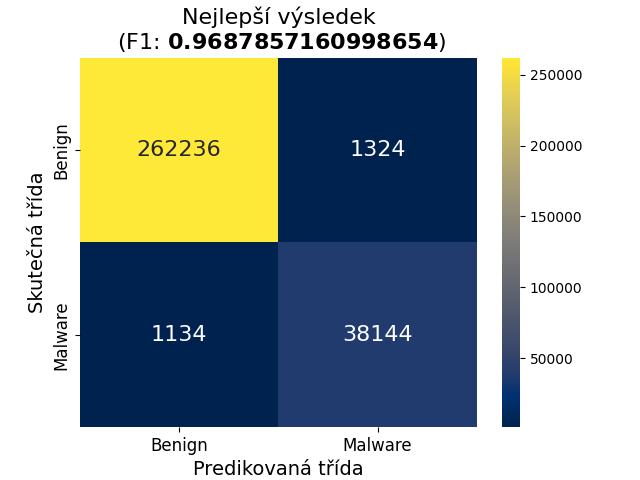
\includegraphics{obrazky-figures/model/best_result_xgb_malware_matrix.png}
		}
		\caption{XGBoost: Matice záměn -- nejlepší výsledek skóre F1 v~10 opakování nad stejnými hyperparametry}
		\label{fig:best_result_xgboost_matrix}
\end{figure}

\begin{figure}[H]
    \centering
		\scalebox{0.75}{
			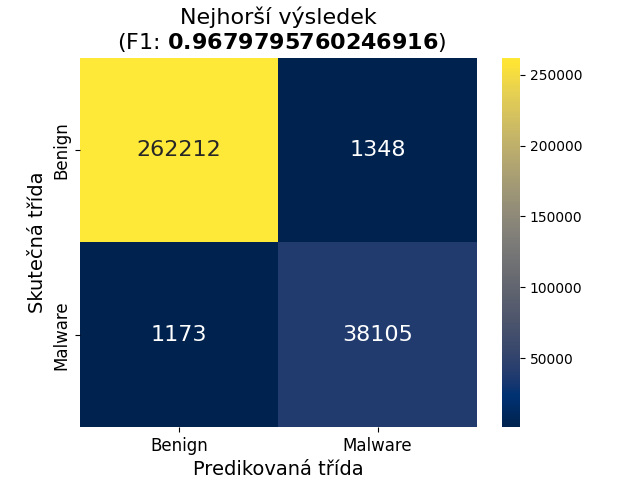
\includegraphics{obrazky-figures/model/worst_result_xgb_malware_matrix.png}
		}
		\caption{XGBoost: Matice záměn -- nejhorší výsledek skóre F1 v~10 opakování nad stejnými hyperparametry}
		\label{fig:worst_result_xgboost_matrix}
\end{figure}

\noindent V~tabulce~\ref{tab:Scikit-learn_classification_report} jsem validoval výsledky na testovací množině k~získání celkového přehledu. Je zde vidět, že model byl validován na sadě o~302 838 doménách a~jeho hodnota skóre F1 vycházela 96.88~\%, což je výsledek velmi podobný průměru, co jsem získal z~testování. Na obrázku~\ref{fig:classification_error} je vidět graf, který zobrazuje míru, s~jakou model nesprávně předpovídá označení tříd, kdy nižší hodnoty znamenají lepší výkonnost. Obrázek~\ref{fig:log_loss} zobrazuje logaritmickou ztrátu, která penalizuje chybné klasifikace a~zase nižší hodnoty jsou lepším výsledkem.
\begin{table}[htbp]
  \centering
    \begin{tabular}{|lcccc|}
    \toprule
    třída & precision & recall & skóre F1 & počet hodnot \\
    \midrule
    benign & 0.9957  & 0.9950  & 0.9954  & 263560 \\
    malware & 0.9665 & 0.9711 & \textbf{0.9688} & 39278 \\
    \midrule
    accuracy &          &         & 0.9919  & 302838 \\
    makro průměr & 0.9811  & 0.9831  & 0.9821  & 302838 \\
    vážený průměr & 0.9919 & 0.9919 & 0.9919 & 302838 \\
    \bottomrule
    \end{tabular}
\caption{XGBoost: Zpráva o~hodnocení klasifikace Scikit-learn}
  \label{tab:Scikit-learn_classification_report}
\end{table}


\begin{figure}[H]
    \centering
		\scalebox{0.75}{
                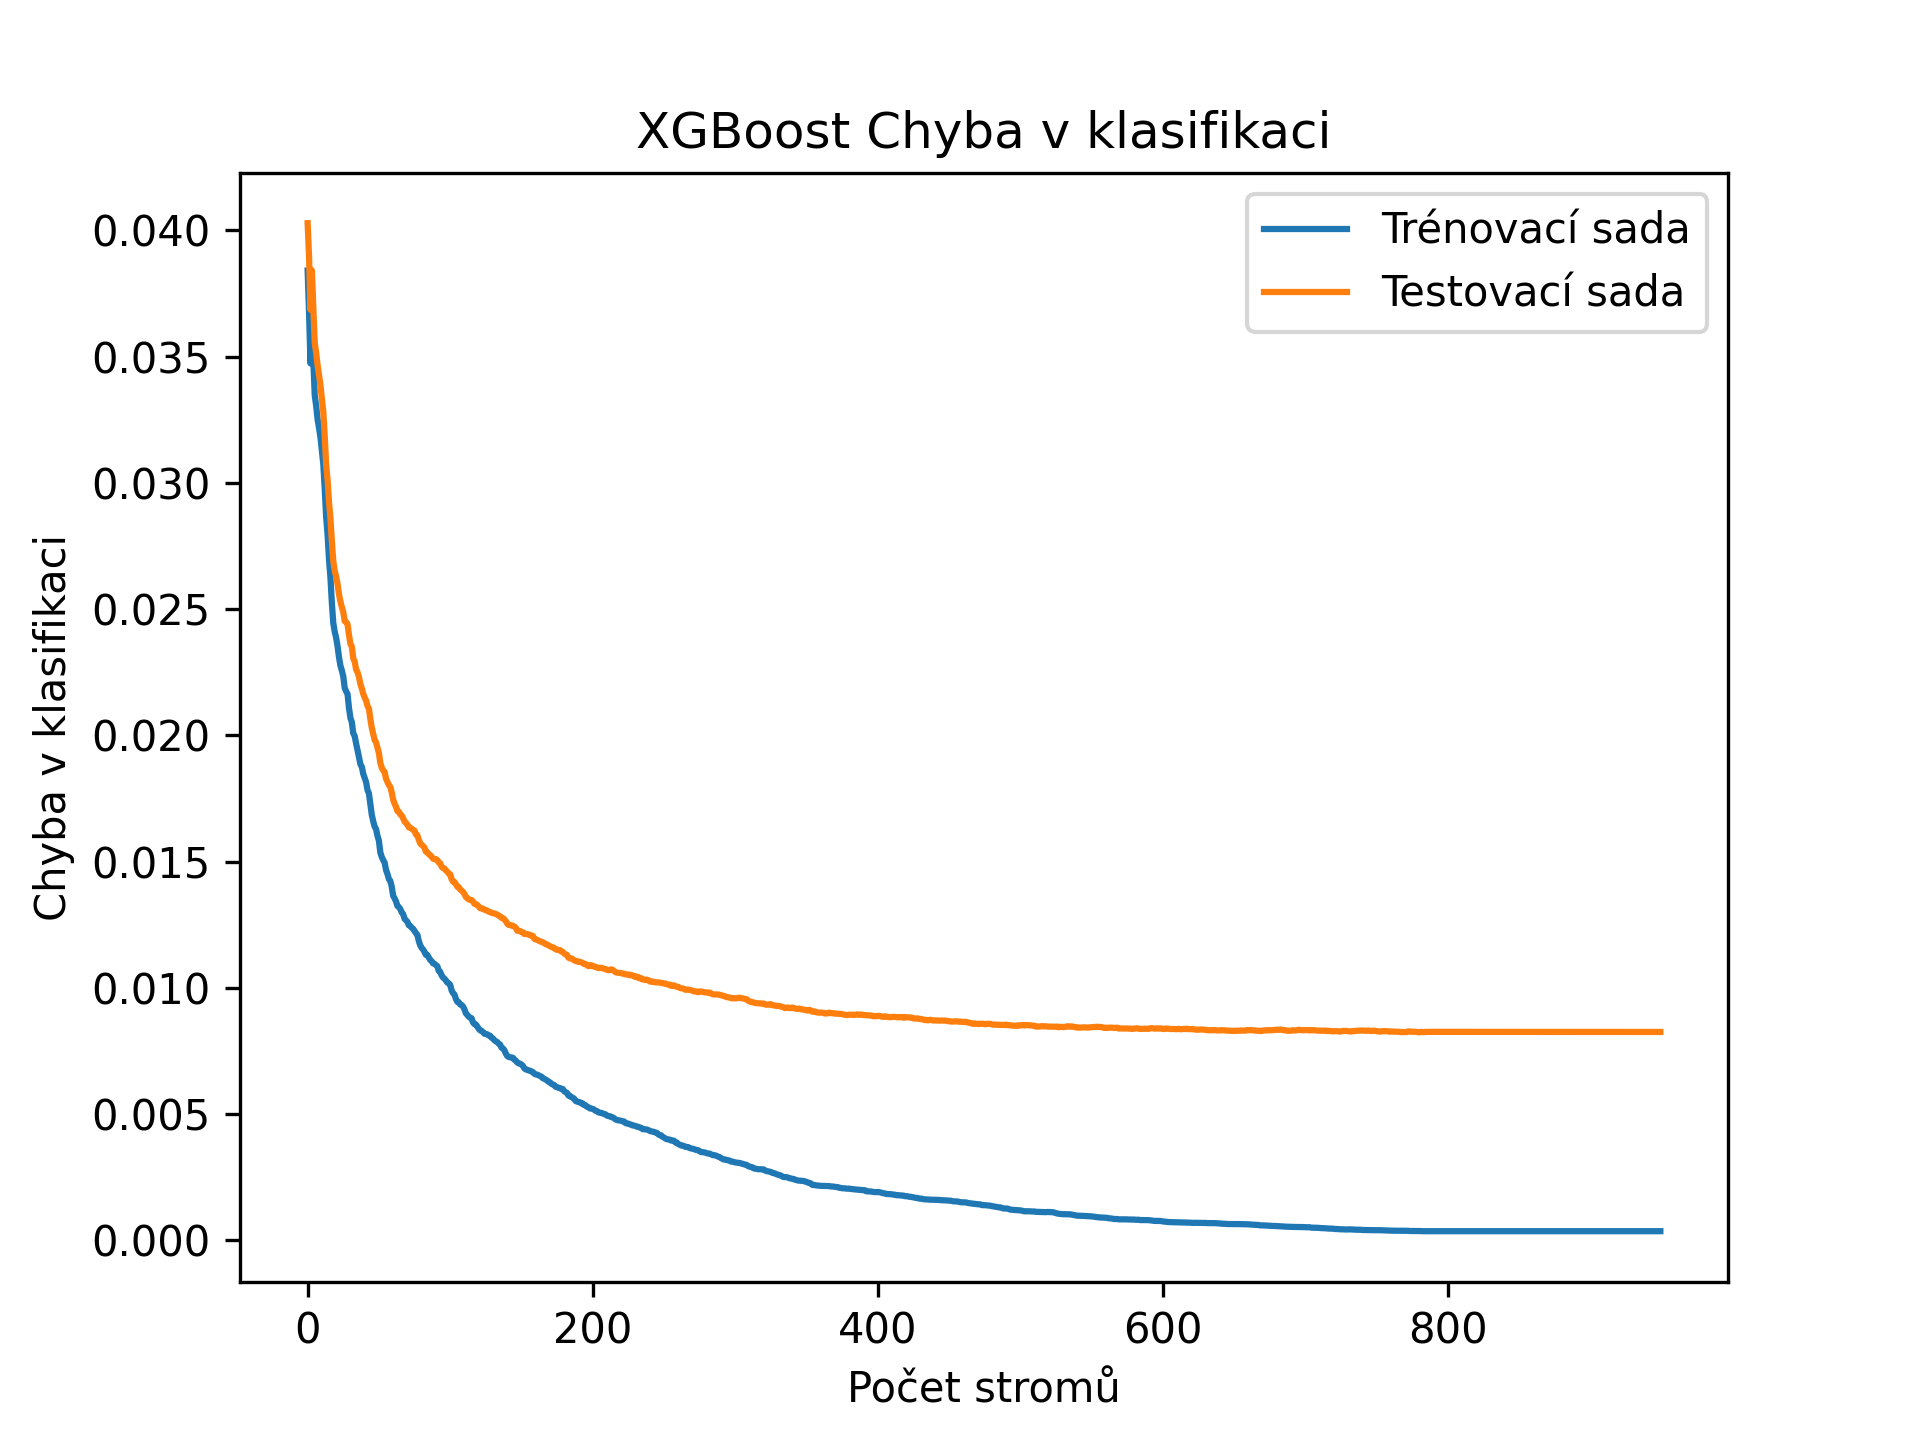
\includegraphics{obrazky-figures/model/Classification_error.png}
		}
		\caption{XGBoost: Graf zobrazující míru, s~jakou klasifikační model nesprávně předpovídá označení tříd. Vypočítá se jako poměr počtu chybně klasifikovaných případů k~celkovému počtu případů. Nižší hodnoty znamenají lepší výkonnost.}
		\label{fig:classification_error}
\end{figure}

\begin{figure}[H]
    \centering
		\scalebox{0.75}{
                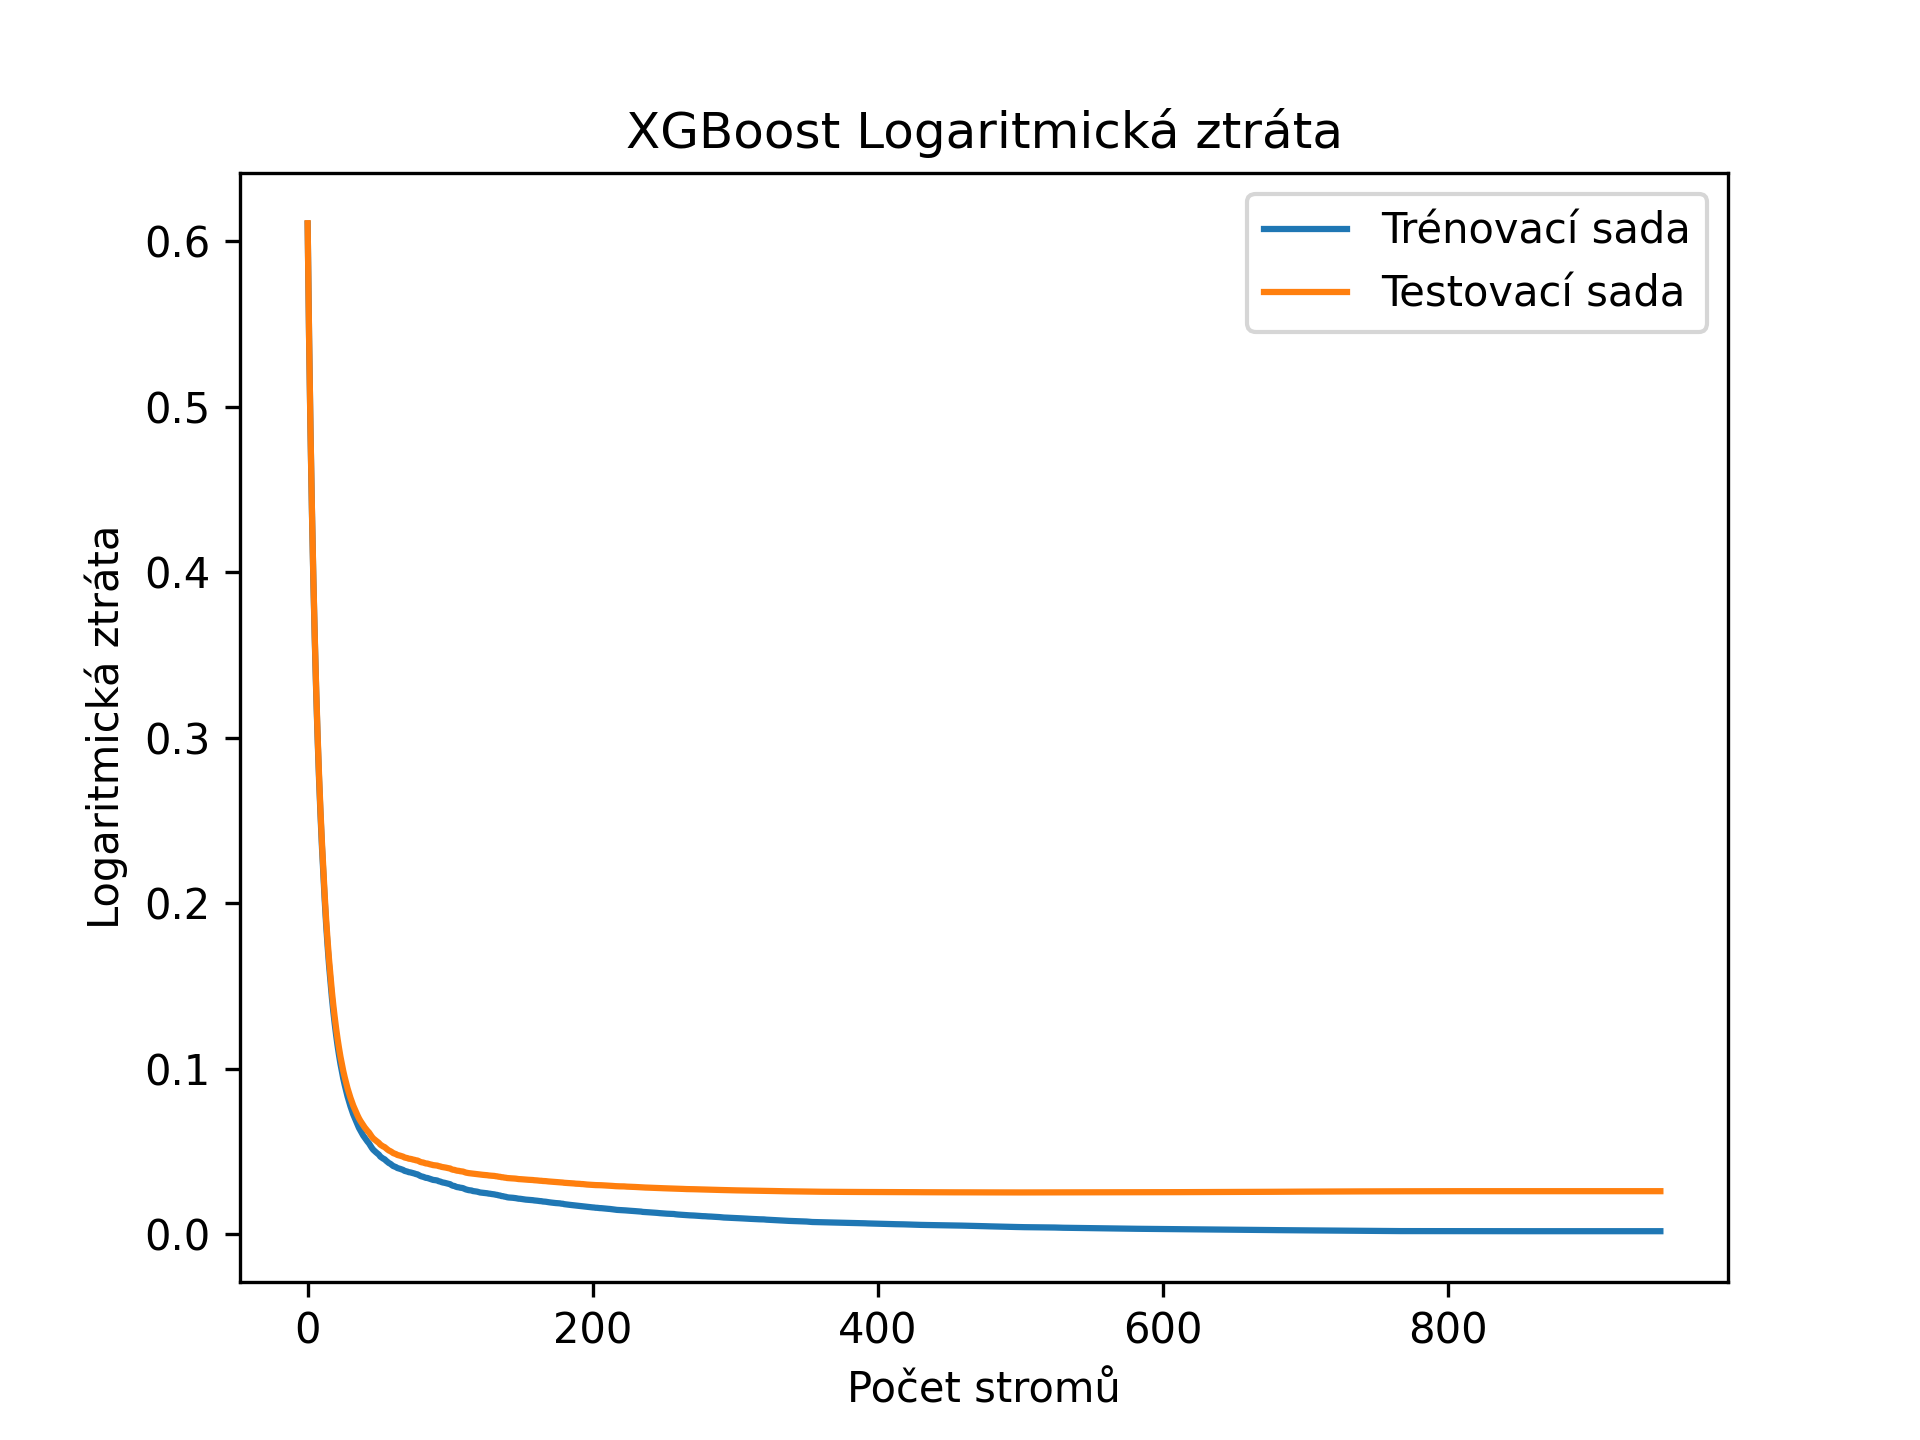
\includegraphics{obrazky-figures/model/Log_Loss.png}
		}
		\caption{XGBoost: Graf zobrazující logaritmickou ztrátu, která penalizuje chybné klasifikace rozdílem mezi skutečnou a~predikovanou pravděpodobností. Nižší hodnoty znamenají lepší výkonnost.}
		\label{fig:log_loss}
\end{figure}


\section{Porovnání s~phishingovým modelem}
Pro porovnání jsem vzal práci Ing. Adama Horáka~\cite{Horak2023thesis}, který trénoval klasifikátor XGBoost na phishingové domény a~dosahoval skóre F1 málo přeš 94~\%. Tento výsledek byl velmi kvalitní i~přes poměrně malou datovou sadu právě zmíněných phishingových domén. Jeho testovací množina u~phishingu právě dosahovala 11 tisíc domén, což v~porovnání s~mými 39 tisíci je nepoměr. Dle mých úsudků vidím můj model jako úspěšnější zejména díky právě počtu získaných domén, což vede často k~lepším výsledkům, neboť klasifikátor má mnohem více možností na vylepšení a~naučení.


%-----------------------------------------------------
% Conclusion
\chapter{Důležitost příznaků} \label{chap:Feature_importance}
V~této kapitole jsou zobrazeny výsledky nejpřínosnějších příznaků pomocí metody \Gls{SHAP} a~také porovnání mezi \Gls{SHAP} a~GAIN, díky čemuž je i~vysvětleno, proč pro moji práci bylo příhodné použít raději \Gls{SHAP} nebo GAIN.

% SHAP results
\section{Přínos příznaků -- SHAP} \label{sec:SHAP_results}
Po získání co nejlepších výsledků jsem se rozhodl, že by bylo příhodné zjistit, jaké příznaky jsou pro tento model nejpřínosnější a~mají největší váhu. Tímto totiž můžu zjistit, jaké příznaky mají při detekci velkou váhu, takže je možné získat díky tomuto přehled, jaké vlastnosti domény mají a~co je pro ně specifické. Zejména pomocí \texttt{summary dot} grafu, který je zmíněn v~části~\ref{subsubsec:SHAP_graphs_summary}, přesněji obrázek~\ref{fig:SHAP_dot}, kde můžeme vidět působení daného příznaku směrem buďto pozitivním nebo negativním, ale i~jakou intenzitou a~frekvencí.

Zároveň při zobrazení všech příznaků a~jejich vlivů je možné detekovat příznaky, které mají pro klasifikaci nulové nebo minimální působení, což při velkém počtu příznaků by bylo příhodné je odstranit, abychom zajistili rychlejší klasifikaci. Já nechával všechny, protože v~mém případě se nejedná ještě o~nějaký obrovský počet, tudíž se mi zdálo zbytečné je odstraňovat. Díky metodě \Gls{SHAP} jsem tedy získal seznam nejvlivnějších příznaků pro natrénovaný model XGBoost, které jsou seřazeny od nejúčinějších:
\begin{itemize}
    \item \texttt{ip\_as\_address\_entropy} -- 1.359,
    \item \texttt{rdap\_ip\_v4\_count} -- 1.357, 
    \item \texttt{lex\_sub\_count} -- 1.267,
    \item \texttt{lex\_tld\_abuse\_score} -- 0.850,
    \item \texttt{ip\_count} -- 0.564,
    \item \texttt{rdap\_domain\_age} -- 0.550,
    \item \texttt{lex\_tld\_hash} -- 0.549,
    \item \texttt{ip\_mean\_average\_rtt} -- 0.505,
    \item \texttt{tls\_expired\_chain} -- 0.492,
    \item \texttt{dns\_A\_count} -- 0.489.
\end{itemize}

Těchto 10 nejlepších příznaků jsem si i~zobrazil pomocí grafů, což u~grafu~\ref{fig:SHAP_top10_bar} je jen vizualizace předchozího seznamu s~přidanými čísly, aby šlo lépe pochopit jak moc daný příznak je vlivný oproti ostatním. U~druhého grafu~\ref{fig:SHAP_top10_dot} už je viditelnější, jaký vliv má na rozhodování určitým směrem, jakou silou a~také jak často. Tyto příznaky vycházejí logicky, když je porovnáme s~výsledky datové analýzy. Ať už se jedná o~nejvíce postižené TLD, kdy u~malware doménových jmen je právě přes 50~\% výskyt \texttt{.com}, což je nejčastěji postižená TLD. Také větší počet poddomén a~IP adres u~benigních doménových jmen.
\begin{figure}[H]
    \centering
		\scalebox{0.59}{
			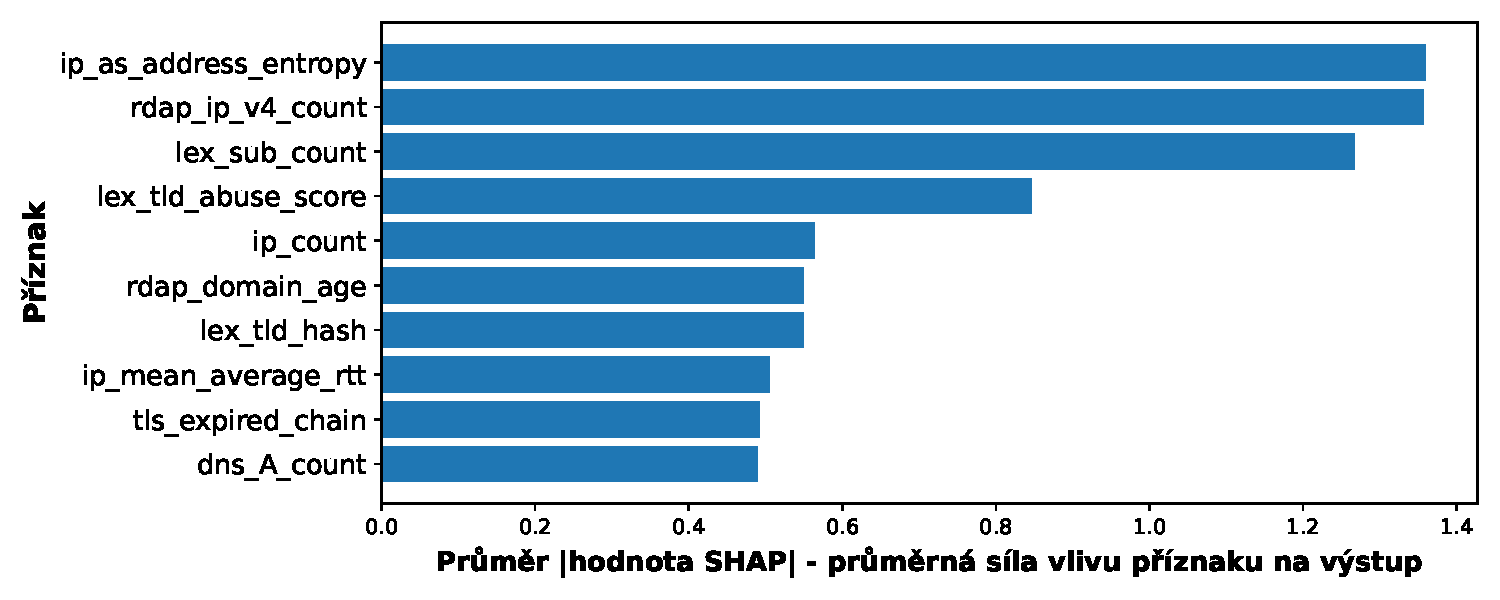
\includegraphics{obrazky-figures/shap/results/shap_top10_bar_xgb_malware.pdf}
		}
		\caption{XGBoost: 10 nejvlivnějších příznaků získaných metodou SHAP zobrazených pomocí summary bar grafu. Tento graf ukazuje průměrnou sílu příznaku nehledě na orientaci vlivu, tudíž zde se nerozlišuje, zda bylo rozhodnutí pro malware nebo benigní. }
		\label{fig:SHAP_top10_bar}
\end{figure}

\begin{figure}[H]
    \centering
		\scalebox{0.59}{
			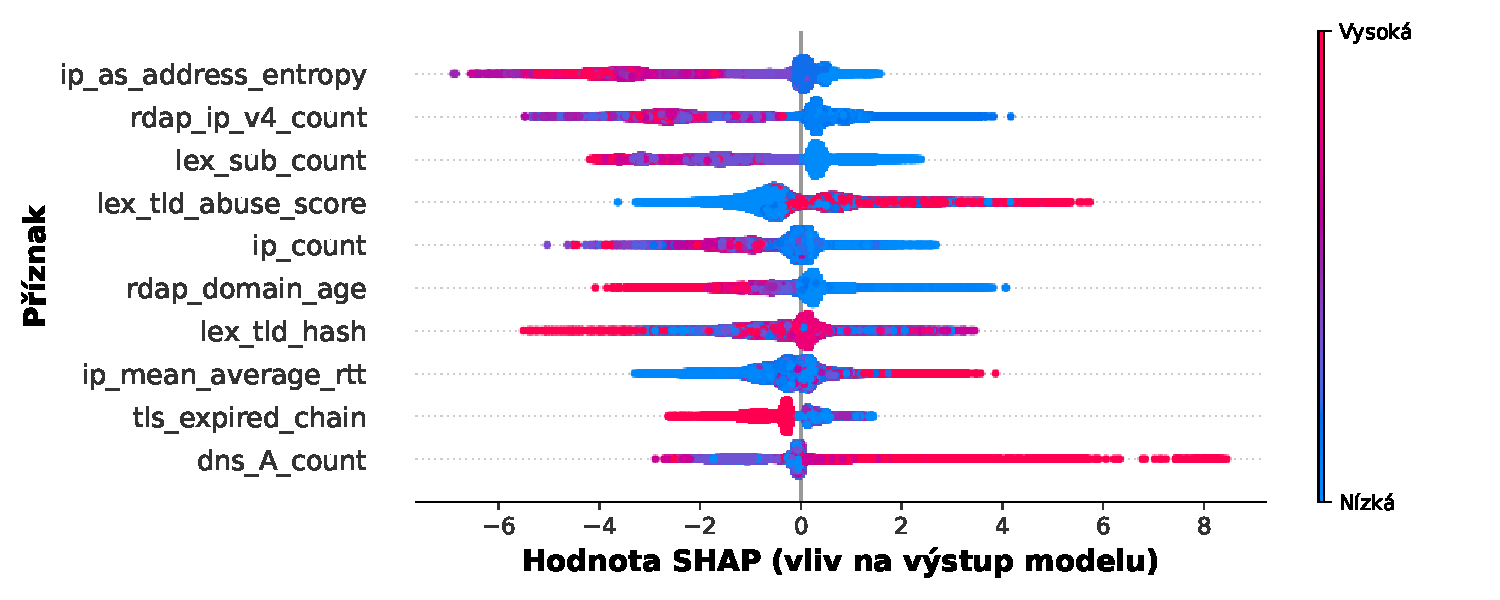
\includegraphics{obrazky-figures/shap/results/shap_top10_dot_xgb_malware.pdf}
		}
		\caption{XGBoost: 10 nejvlivnějších příznaků získaných metodou SHAP zobrazených pomocí summary dot grafu. Tento graf ukazuje vlivy na výstup modelu, kdy pomohl při rozhodování, jestli doména bude malware nebo benigní. Ukazuje také intenzitu a~frekvenci vlivu.}
		\label{fig:SHAP_top10_dot}
\end{figure}

\section{Porovnání výsledků GAIN a~SHAP}
Aby bylo možné říci, který nástroj na zjišťování nejlepších příznaků je tou správnou volbou, je nutné si to otestovat. Zjistil jsem pomocí každé metody 10 nejlepších příznaků a~poté jsem pouze s~těmito příznaky trénoval model, který jsem následně otestoval na validační množině. V~tabulce~\ref{tab:SHAP_vs_GAIN_comparsion} jsem zobrazil výsledky, které jsou důkazem, že pro moji práci se více hodí metoda \Gls{SHAP}, která určuje příznaky více relevantně, což je dokázáno i~tím, že při použití jen těchto 10 nejlepších příznaků klasifikátor dosahuje lepších výsledků než je tomu příznaků z~metody GAIN.

\begin{table}[h]
\begin{tabular}{c|cc|cc|cc|c|c|}
\cline{2-9}
                           & \multicolumn{2}{c|}{Precision}       & \multicolumn{2}{c|}{Recall}          & \multicolumn{2}{c|}{F1}              & \multirow{2}{*}{Accuracy} & \multirow{2}{*}{\Gls{FPR}} \\ \cline{2-7}
                           & \multicolumn{1}{c|}{N}      & P      & \multicolumn{1}{c|}{N}      & P      & \multicolumn{1}{c|}{N}      & P      &                     &                     \\ \hline
\multicolumn{1}{|l|}{SHAP} & \multicolumn{1}{l|}{0.9939} & 0.8791 & \multicolumn{1}{l|}{0.9803} & 0.9596 & \multicolumn{1}{l|}{0.9871} & \textbf{0.9176} & 0.9776              & \textbf{0.01966}                \\ \hline
\multicolumn{1}{|l|}{GAIN} & \multicolumn{1}{l|}{0.9886} & 0.6585 & \multicolumn{1}{l|}{0.9283} & 0.9279 & \multicolumn{1}{l|}{0.9575} & \textbf{0.7703} & 0.9282              & \textbf{0.07171}                \\ \hline
\end{tabular}
\caption{XGBoost: Výsledky trénování modelů jen na top 10 příznacích získaných z~GAIN a~SHAP}
\label{tab:SHAP_vs_GAIN_comparsion}
\end{table}

\noindent Na obrázku~\ref{fig:SHAP-SHAP_vs_GAIN} je možné vidět normalizované hodnoty jak u~\Gls{SHAP}, tak i~GAIN, kde vybrání 10 nejlepších příznaků bylo provedeno pomocí \Gls{SHAP}. NA obrázku~\ref{fig:GAIN-SHAP_vs_GAIN} je to zase naopak a~příznaky jsou vybrány pomocí GAIN.
\begin{figure}[H]
    \centering
		\scalebox{0.58}{
			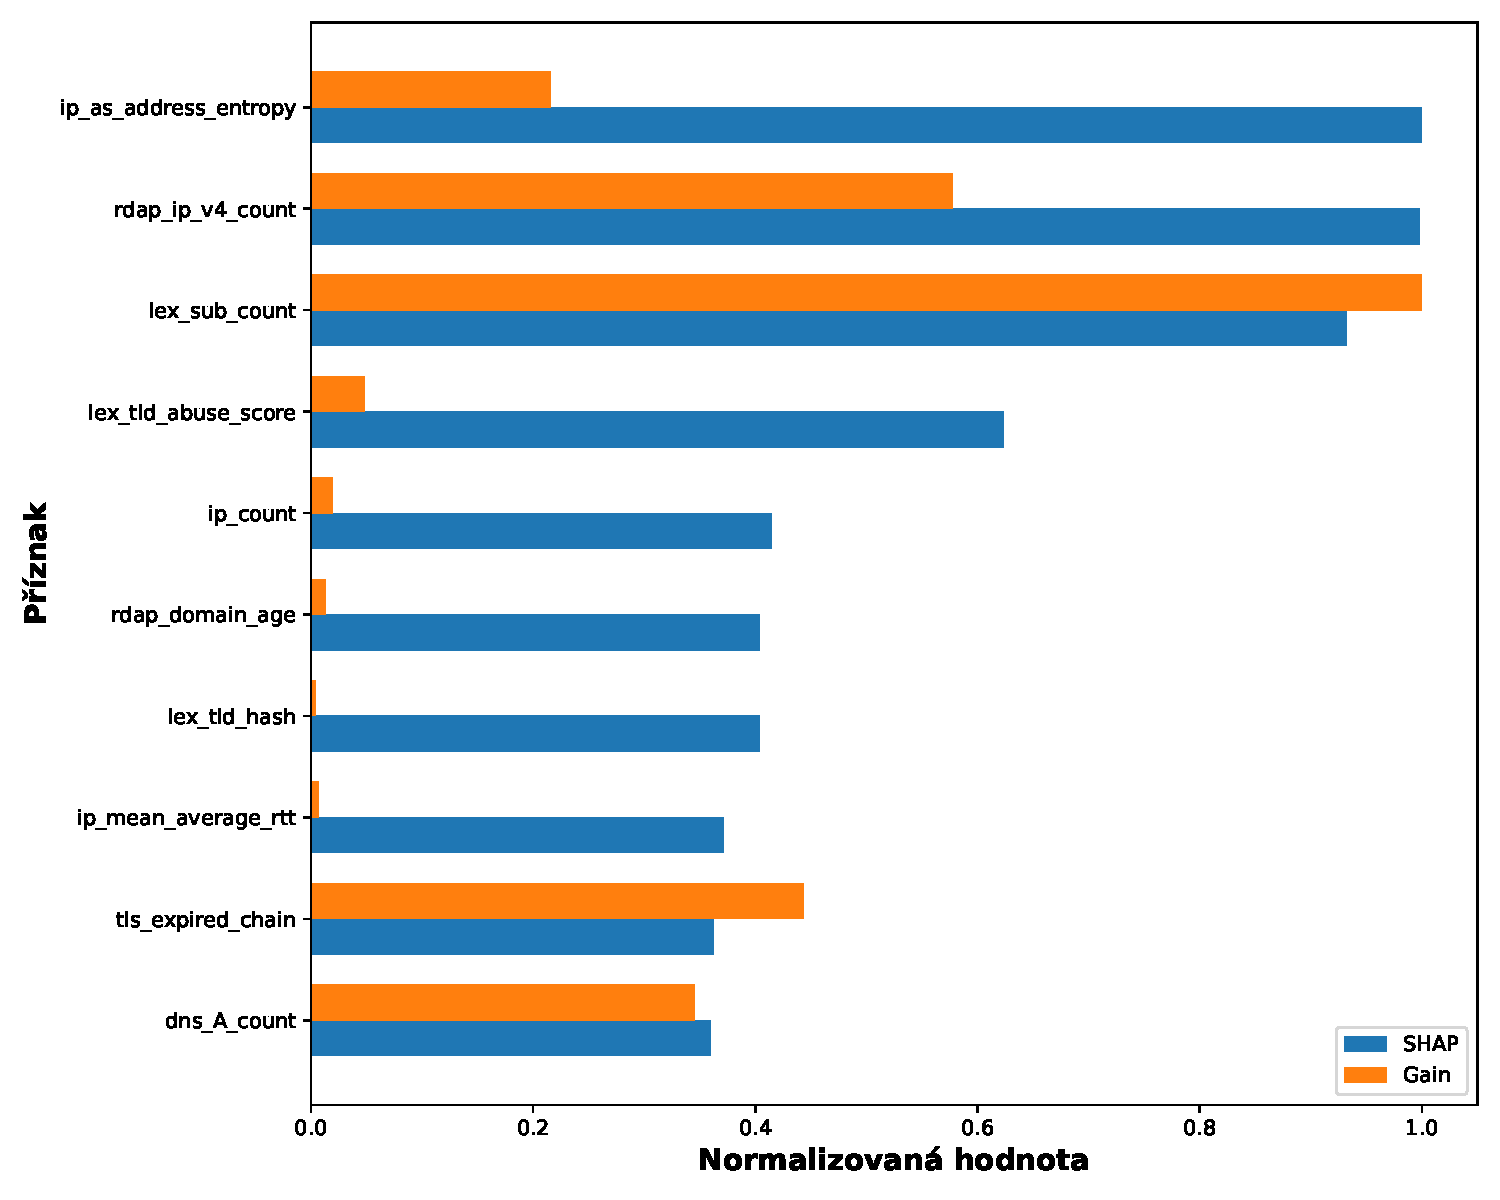
\includegraphics{obrazky-figures/shap/results/SHAP_GAIN_compare_by_SHAP.pdf}
		}
		\caption{XGBoost: 10 nejvlivnějších příznaků získaných metodou SHAP v~porovnání s~jejich hodnotami získanými z~GAIN}
		\label{fig:SHAP-SHAP_vs_GAIN}
\end{figure}

\begin{figure}[H]
    \centering
		\scalebox{0.59}{
			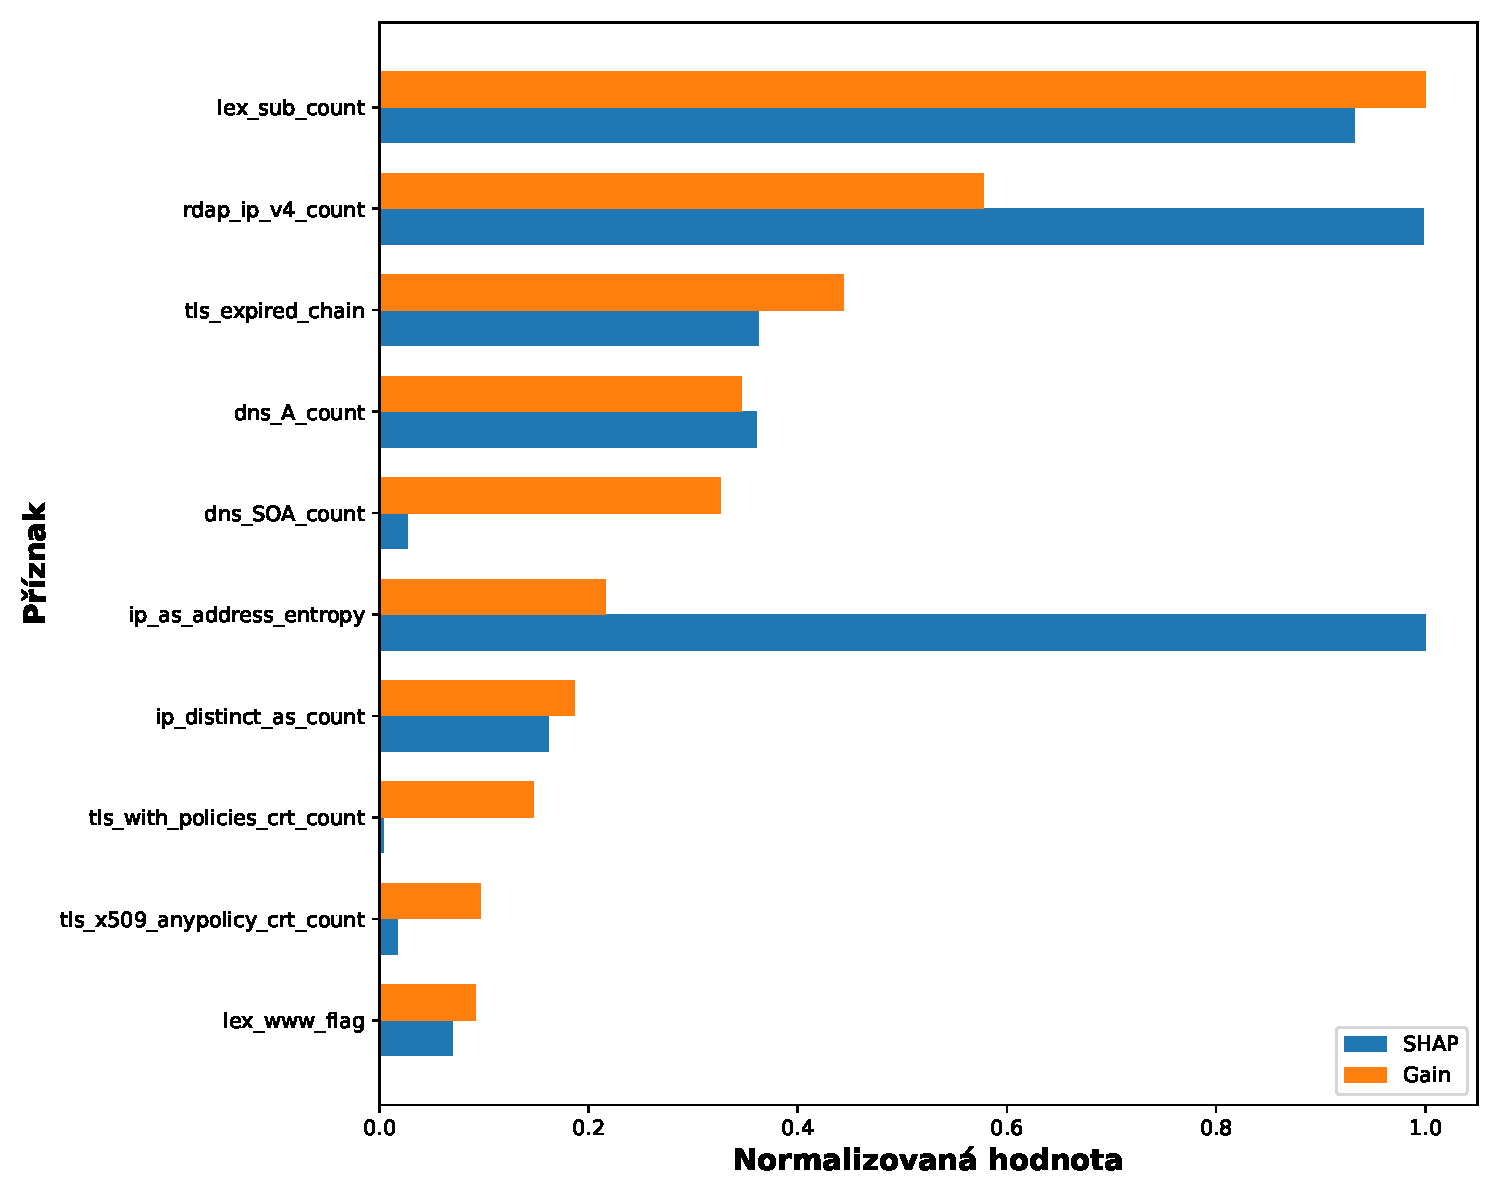
\includegraphics{obrazky-figures/shap/results/SHAP_GAIN_compare_by_GAIN.pdf}
		}
		\caption{XGBoost: 10 nejvlivnějších příznaků získaných metodou GAIN v~porovnání s~jejich hodnotami získanými ze SHAP}
		\label{fig:GAIN-SHAP_vs_GAIN}
\end{figure}


%-----------------------------------------------------
% Conclusion
\chapter{Závěr} \label{chap:Conclusion}
Cílem této bakalářské práce bylo vytvořit datovou sadu malware domén a~následně model, který bude detekce tyto domény. K~tomuto bylo zapotřebí prostudovat danou problematiku a~to zejména v~oblasti klíčových externích zdrojů dat o~doménách (\Gls{DNS}, \Gls{RDAP} atd.), ale také již dostupná řešení, která mohou řešit podobná témata a~je možné zjistit, jaké přístupy využívali a~jakých výsledků dosahovali.

Klíčovým prvkem byl sběr dat, kde bylo nutné čerpat z~aktivních zdrojů, které pravidelně poskytují domény, ale i~z~různých fór a~účtů na GitHub, které poskytují černé listiny domén detekovaných jako malware. Našel jsem mnoho černých listin s~mnohdy velkým počtem detekovaných domén, které se však velmi často zúžily třeba i~na polovinu, neboť jsem u~nich prováděl nejen kontrolu, zda je doména živá, abych z~ní mohl získat co nejvíce dat, ale také, zda se jedná opravdu o~malware. I~přes tyto komplikace se stalo mým největším přínosem rozšíření datové sady malware domén z~původních 46 tisíc na 131 tisíc domén.

Neméně důležitou částí pak bylo trénování a~testování různých klasifikátorů a~snaha získat nejlepší výsledky. Bylo odzkoušeno 8 různých klasifikátorů a~jejich zlepšování, kdy byl následně vybrán jeden k~podrobné analýze a~snaze získat nejlepší výsledky. To je možné pomocí vylepšování hyperparametrů a~k~tomu sloužily hledací algoritmy jako například Random Search, Grid Search a~nebo Bayesan Search. Posledním krokem bylo zjišťování nejužitečnějších příznaků, které pro tuto detekci měli největší přínos a~díky tomu i~možné porovnání s~phishingovým modelem pro detekci z~práce Adama Horáka.

 Souhrnně tedy díky kvalitní datové sadě s~mnoha záznamy a~vylepšeným modelem jsem byl schopný získat u~nejlepšího modelu skóre F1 při testování 96.8786~\% s~poměrem falešně detekovaných pozitivních domén 0.004887.

Cílem mé budoucí práce je sběr dalších dat. Zejména najití stránek, které dávají pravidelně kvalitní domény, které budou sloužit pro lepší natrénování modelu. Tím by mohla vzniknout i~preciznější datová analýza, ze které by vycházely jasnější výsledky, kdy například by u~malware domén nemusely často chybět IPv6 záznamy, což může být způsobeno stářím domény. Také bych se chtěl zaměřit na detekci celé URL, neboť v~tom vidím potenciál detekce jen části domén a~vyhnutí se blokování domén, které mají jen v~určitých částech malware, například vložený uživatelem. Poslední částí je zajisté i~vylepšování dosavadních klasifikátorů, hledání lepších parametrů, ale i~například zkoušení úplně nových klasifikátorů. Také by bylo velmi dobré se zaměřit směrem k~obsahu HTML/DOM jako zdroj příznaků, což by eliminovalo problém, která může nastat, když je doména infikována jen na dobu určitou. 
%===============================================================================

% Pro kompilaci po částech (viz projekt.tex) nutno odkomentovat
%\end{document}

  \fi
  
  % Kompilace po částech (viz výše, nutno odkomentovat a zakomentovat input výše)
  % Compilation piecewise (see above, it is necessary to uncomment it and comment out input above)
  %\subfile{chapters/projekt-01-uvod-introduction}
  % ...
  %\subfile{chapters/projekt-05-zaver-conclusion}

  % Pouzita literatura / Bibliography
  % ----------------------------------------------
\ifslovak
  \makeatletter
  \def\@openbib@code{\addcontentsline{toc}{chapter}{Literatúra}}
  \makeatother
  \bibliographystyle{bib-styles/Pysny/skplain}
\else
  \ifczech
    \makeatletter
    \def\@openbib@code{\addcontentsline{toc}{chapter}{Literatura}}
    \makeatother
    \bibliographystyle{bib-styles/Pysny/czplain}
  \else 
    \makeatletter
    \def\@openbib@code{\addcontentsline{toc}{chapter}{Bibliography}}
    \makeatother
    \bibliographystyle{bib-styles/Pysny/enplain}
  %  \bibliographystyle{alpha}
  \fi
\fi
  \begin{flushleft}
  \bibliography{xebert00-20-literatura-bibliography}
  \end{flushleft}

  % vynechani stranky v oboustrannem rezimu
  % Skip the page in the two-sided mode
  \iftwoside
    \cleardoublepage
  \fi

  % Prilohy / Appendices
  % ---------------------------------------------
  \appendix
\ifczech
  \renewcommand{\appendixpagename}{Přílohy}
  \renewcommand{\appendixtocname}{Přílohy}
  \renewcommand{\appendixname}{Příloha}
\fi
\ifslovak
  \renewcommand{\appendixpagename}{Prílohy}
  \renewcommand{\appendixtocname}{Prílohy}
  \renewcommand{\appendixname}{Príloha}
\fi
%  \appendixpage

% vynechani stranky v oboustrannem rezimu
% Skip the page in the two-sided mode
%\iftwoside
%  \cleardoublepage
%\fi
  
\ifslovak
%  \section*{Zoznam príloh}
%  \addcontentsline{toc}{section}{Zoznam príloh}
\else
  \ifczech
%    \section*{Seznam příloh}
%    \addcontentsline{toc}{section}{Seznam příloh}
  \else
%    \section*{List of Appendices}
%    \addcontentsline{toc}{section}{List of Appendices}
  \fi
\fi
  \startcontents[chapters]
  \setlength{\parskip}{0pt} 
  % seznam příloh / list of appendices
  % \printcontents[chapters]{l}{0}{\setcounter{tocdepth}{2}}
  
  \ifODSAZ
    \setlength{\parskip}{0.5\bigskipamount}
  \else
    \setlength{\parskip}{0pt}
  \fi
  
  % vynechani stranky v oboustrannem rezimu
  \iftwoside
    \cleardoublepage
  \fi
  
  % Přílohy / Appendices
  \ifenglish
    \input{xebert00-30-prilohy-appendices-en}
  \else
    % Tento soubor nahraďte vlastním souborem s přílohami (nadpisy níže jsou pouze pro příklad)

\chapter{Obsah přiloženého paměťového média}
Přiložené médium obsahuje:
    \begin{itemize}
        \item tento soubor ve formátu PDF,
        \item zdrojové kódy (\LaTeX) této práce,
        \item kompletní zdrojové kódy pro sběr dat,
        \item kompletní zdrojové kódy pro extrakci příznaků,
        \item kompletní zdrojové kódy pro trénování klasifikátorů,
        \item manuál k použití.
    \end{itemize}
        

\chapter{Seznam příznaků}
V~této příloze se nachází tabulka~\ref{tab:all_features}, která zobrazuje seznam příznaků seřazených podle vlivu a důležitosti podle SHAP. V~prvním sloupci je samostatná hodnota SHAP, v~dalším je kategorie do které daný příznak spadá, poté i jeho celé jméno, jak je v~kódu a v~posledním sloupci je vysvětlení, co daný příznak znamená.

V~tabulce jsou použity i zkratky, proto zde je výpis těch, které nemusí být na první pohled patrné:
\begin{itemize}
    \item SLD -- doména druhé úrovně,
    \item TLD -- doména první úrovně,
    \item DN -- doménové jméno,
    \item RR -- zdrojový záznam v~DNS (A, AAAA, ...),
    \item SAN -- alternativní názvy subjektů,
    \item AS -- autonomní systém,
    \item NS -- name server,
    \item VPS -- virtuální privátní server.
\end{itemize}
\begin{landscape}
\begin{center}
        \begin{longtable}{|l|l|l|p{10cm}|}
        \caption{Seznam příznaků využitých pro klasifikátory} \label{tab:all_features} \\
    
        \hline 
        \multicolumn{1}{|c|}{\textbf{SHAP}} & 
        \multicolumn{1}{c|}{\textbf{Kategorie}} & 
        \multicolumn{1}{c|}{\textbf{Název příznaku v~kódu}} & 
        \multicolumn{1}{c|}{\textbf{Význam příznaku}} \\ 
        \hline 
        \endfirsthead

        \caption{Seznam příznaků využitých pro klasifikátory} \\
        \hline 
        \multicolumn{1}{|c|}{\textbf{SHAP}} & \multicolumn{1}{c|}{\textbf{Kategorie}} & \multicolumn{1}{c|}{\textbf{Název příznaku v~kódu}} & \multicolumn{1}{c|}{\textbf{Význam příznaku}} \\ \hline 
        \endhead
        
        \hline \hline
        \endfoot    
        
        \hline \hline
        \endlastfoot
        
        1.359 & IP & ip\_as\_address\_entropy & entropie IP prefixů AS \\
        1.357 & RDAP & rdap\_ip\_v4\_count & počet IPv4 adres v~RDAP \\
        1.267 & lexikální & lex\_sub\_count & počet subdomén \\
        0.850 & lexikální & lex\_tld\_abuse\_score & skóre pro nejpoužívanější TLD \\ 
        0.564 & IP & ip\_count & počet IP adres \\
        0.550 & RDAP & rdap\_domain\_age & počet dní od registrace domény \\
        0.549 & lexikální & lex\_tld\_hash & hash TLD \\
        0.505 & IP & ip\_mean\_average\_rtt & průměrná RTT všech pokusů ICMP Echo \\ 
        0.492 & TLS & tls\_expired\_chain & příznak, zda je v~řetězci certifikát s~prošlou platností \\
        0.489 & DNS & dns\_A\_count & počet záznamů A~\\
        0.459 & lexikální & lex\_tld\_len & délka TLD \\
        0.447 & RDAP & rdap\_time\_from\_last\_change & počet dní od poslední změny \\
        0.413 & RDAP & rdap\_registrar\_name\_len & délka jména registrátora \\
        0.410 & RDAP & rdap\_registrar\_name\_hash & hash jména registrátora \\
        0.385 & IP & ip\_entropy & celková entropie všech /16 (/64 pro v6) IP prefixů\\
        0.382 & DNS & dns\_NS\_count & počet záznamů NS \\
        0.359 & TLS & tls\_chain\_len & délka řetězce certifikátu \\
        0.349 & DNS & dns\_ttl\_stdev & směrodatná odchylka TTL v~rámci sady RRset \\
        0.308 & DNS & dns\_zone\_entropy & normalizovaná entropie zóny DN \\
        0.271 & DNS & dns\_zone\_len & počet znaků v~zóně DN \\
        0.270 & IP & ip\_v4\_ratio & poměr IPv4 ke všem IP adresám \\
        0.260 & RDAP & rdap\_registration\_period & rozdíl mezi datem vypršení platnosti a datem registrace \\
        0.223 & RDAP & rdap\_registrar\_name\_entropy & entropie jména registrátora \\
        0.219 & IP & ip\_distinct\_as\_count & počet různých AS \\
        0.191 & DNS & dns\_ttl\_low & pčet sad RR s~TTL $\in [0, 100]$  \\
        0.184 & lexikální & lex\_stdev\_part\_lens & směrodatná odchylka délky částí doménového jména \\
        0.183 & DNS & dns\_ttl\_avg & průměrná hodnota TTL napříč sadami RRs  \\
        &&&\\        
        \multirow{3}{*}{0.181} & \multirow{3}{*}{TLS} & \multirow{3}{*}{tls\_joint\_isoitu\_policy\_crt\_count} & počet certifikátů s~politikou z~Joint ISO ITU-T \\
        & & & \textit{certifikáty s~rozšířením Certificate Policies, které obsahují politiku s~OID z~Joint ISO ITU-T podstromu (2)} \\
        0.173 & RDAP & rdap\_ip\_avg\_admin\_name\_len & průměrná délka jména správce pro IP adresy \\
        0.167 & DNS & dns\_ttl\_distinct\_count & počet různých hodnot TTL v~sadách RRsets \\
        0.160 & DNS & dns\_MX\_count & počet záznamů MX \\
        0.143 & RDAP & rdap\_ip\_avg\_admin\_email\_entropy & průměrná entropie e-mailu správce pro IP adresu \\
        0.134 & DNS & dns\_soa\_retry & SOA retry parametr \\
        0.125 & lexikální & lex\_malware\_pentagram\_matches & počet běžných shod malwarových pentagramů v~DN \\
        0.124 & RDAP & rdap\_domain\_active\_time & min(dnešní datum, expirace) - datum registrace \\
        0.123 & geolokace & geo\_countries\_hash & jedinečný hash pro každou kombinaci zemí  \\
        0.119 & RDAP & rdap\_ip\_shortest\_v4\_prefix\_len & délka nejkratšího prefixu IPv4 \\ 
        0.117 & lexikální & lex\_malware\_bigram\_matches & počet běžných shod malwarových bigramů v~DN \\
        0.115 & RDAP & rdap\_ip\_v6\_count & počet IPv6 adres v~RDAP \\
        0.113 & lexikální & lex\_avg\_part\_len & průměrná délka částí doménového jména \\
        0.112 & DNS & dns\_AAAA\_count & počet záznamů AAAA \\
        0.111 & lexikální & lex\_sub\_hex\_ratio & poměr hexadecimálních symbolů v~subdoménách \\
        0.111 & lexikální & lex\_sld\_norm\_entropy & normalizovaná entropie SLD \\
        0.103 & RDAP & rdap\_ip\_avg\_admin\_name\_entropy & průměrná entropie e-mailu správce pro IP adresu \\
        0.103 & lexikální & lex\_stld\_unique\_char\_count & počet jedinečných znaků v~TLD a SLD \\
        0.103 & lexikální & lex\_malware\_tetragram\_matches & počet běžných shod malwarových tetragramů v~DN \\
        0.097 & TLS & tls\_leaf\_authority\_hash & hash názvu listové certifikační autority \\
        0.095 & lexikální & lex\_sld\_hex\_ratio & poměr hexadecimálních symbolů v~SLD \\
        0.095 & lexikální & lex\_www\_flag & doména začíná na www \\
        0.094 & RDAP & rdap\_ip\_avg\_admin\_email\_len & průměrná délka e-mailu správce pro IP adresy \\
        0.093 & geolokace & geo\_max\_lon & maximální zeměpisná délka míst IP \\
        0.092 & RDAP & rdap\_ip\_longest\_v4\_prefix\_len & délka nejdelšího prefixu IPv4 \\
        0.091 & lexikální & lex\_sld\_vowel\_ratio & poměr samohlásek v~SLD \\  
        0.091 & lexikální & lex\_malware\_trigram\_matches & počet běžných shod malwarových trigramů v~DN \\
        0.090 & TLS & tls\_negotiated\_cipher\_id & identifikátor vyjednané šifry TLS \\
        0.089 & lexikální & lex\_sub\_non\_alphanum\_ratio & poměr podtržítek a pomlček v~subdoménách \\
        0.087 & lexikální & lex\_sub\_vowel\_ratio & poměr samohlásek v~subdoménách \\
        0.086 & lexikální & lex\_sub\_norm\_entropy & normalizovaná entropie subdomén \\
        0.082 & lexikální & lex\_sub\_consonant\_ratio & poměr souhlásek v~subdoménách \\
        0.081 & DNS & dns\_txt\_avg\_entropy & průměrná normalizovaná entropie hodnot TXT RRs \\
        0.081 & DNS & dns\_soa\_refresh & SOA refresh parametr \\
        0.079 & lexikální & lex\_sld\_consonant\_ratio & poměr souhlásek v~SLD \\
        0.079 & DNS & dns\_mx\_avg\_len & průměrný počet znaků v~záznamech MX DN \\
        0.077 & lexikální & lex\_sub\_max\_consonant\_len & nejdelší délka souhláskové sekvence v~subdoménách \\
        0.076 & DNS & dns\_soa\_min\_ttl & SOA minimum TTL \\
        0.075 & DNS & dns\_CNAME\_count & počet záznamů CNAME \\
        0.075 & DNS & dns\_resolved\_record\_types & počet nalezených souborů RR \\ 
        0.069 & RDAP & rdap\_ip\_longest\_v6\_prefix\_len & délka nejdelšího prefixu IPv6 \\
        0.069 & lexikální & lex\_name\_len & délka doménového jména \\    
        0.069 & DNS & dns\_mx\_avg\_entropy & průměrná normalizovaná entropie v~záznamech MX DN \\
        0.064 & DNS & dns\_has\_dnskey & příznak, zda se v~zóně nachází sada DNSKEY RRset \\
        0.064 & TLS & tls\_negotiated\_version\_id & číslo vyjednané verze TLS (TLSv1.x) \\
        0.064 & geolokace & geo\_min\_lat & minimální zeměpisná délka míst IP \\
        0.056 & geolokace & geo\_max\_lat & maximální zeměpisná délka míst IP \\
        0.056 & TLS & tls\_root\_authority\_hash & hash názvu kořenové certifikační autority \\ 
        0.055 & TLS & tls\_total\_extension\_count & celkový počet rozšíření ve všech certifikátech v~řetězci \\
        0.055 & RDAP & rdap\_registrant\_name\_len & délka jména žadatele o~registraci \\
        0.055 & DNS & dns\_soa\_primary\_ns\_entropy & normalizovaná entropie primárního NS DN \\
        0.054 & DNS & dns\_TXT\_count & počet záznamů TXT \\   
        0.054 & lexikální & lex\_consecutive\_chars & nejdelší po sobě jdoucí délka sekvence \\
        0.053 & geolokace & geo\_min\_lon & minimální zeměpisná délka míst IP \\
        0.053 & RDAP & rdap\_ip\_shortest\_v6\_prefix\_len & délka nejkratšího prefixu IPv6 \\
        0.051 & DNS & dns\_soa\_email\_entropy & normalizovaná entropie e-mailu správce DN  \\ 
        0.049 & RDAP & rdap\_registrant\_name\_entropy & entropie názvu žadatele o~registraci \\
        \multirow{2}{*}{0.047} & \multirow{2}{*}{TLS} & \multirow{2}{*}{tls\_critical\_extensions} & celkový počet rozšíření označených jako "kritická" ve všech certifikátech \\
        0.046 & DNS & dns\_soa\_primary\_ns\_len & počet znaků v~DN primárního NS \\    
        0.044 & IP & ip\_asn\_entropy & entropie čísel AS \\
        0.044 & geolokace & geo\_lon\_range & rozsah zeměpisné délky \\
        0.042 & DNS & dns\_ttl\_mid & počet sad RR s~TTL $\in [101, 500]$ \\
        0.042 & geolokace & geo\_centroid\_lon & střední zeměpisná délka míst IP \\ 
        0.042 & lexikální & lex\_sub\_consonant\_count & počet souhlásek v~subdoménách \\ 
        0.041 & lexikální & lex\_shortest\_sub\_len & nejkratší délka subdomény \\
        0.040 & lexikální & lex\_sld\_len & délka SLD \\
        0.039 & lexikální & lex\_sld\_non\_alphanum\_ratio & poměr podtržítek a pomlček v~SLD \\
        0.038 & lexikální & lex\_sld\_digit\_ratio & poměr číslic v~SLD \\
        0.038 & geolokace & geo\_mean\_lon & průměrná zeměpisná délka míst IP \\
        0.038 & lexikální & lex\_sld\_vowel\_count & počet samohlásek v~SLD \\
        0.038 & geolokace & geo\_mean\_lat & střední zeměpisná šířka míst IP \\
        0.037 & DNS & dns\_SOA\_count & počet záznamů SOA \\
        0.036 & DNS & dns\_soa\_expire & parametr vypršení platnosti záznamu SOA \\
        0.036 & lexikální & lex\_sld\_hex\_count & počet hexadecimálních symbolů v~SLD \\
        0.036 & lexikální & lex\_longest\_part\_len & délka nejdelší části názvu domény \\
        0.035 & geolokace & geo\_continent\_hash & jedinečný hash pro každou kombinaci kontinentů \\
        0.035 & lexikální & lex\_sld\_consonant\_count & počet souhlásek v~SLD \\
        0.034 & DNS & dns\_domain\_name\_in\_mx & příznak, zda je některý poštovní server subdoménou DN \\
        0.033 & lexikální & lex\_sub\_digit\_count & počet číslic v~subdoménách \\
        0.032 & lexikální & lex\_sub\_hex\_count & počet hexadecimálních symbolů v~subdoménách \\
        0.032 & geolokace & geo\_lon\_stdev & směrodatná odchylka od zeměpisných délek míst IP \\
        0.031 & DNS & dns\_soa\_primary\_ns\_digit\_count & počet číslic v~primárním NS DN \\
        0.030 & lexikální & lex\_sub\_digit\_ratio & poměr číslic v~subdoménách \\
        0.030 & RDAP & rdap\_admin\_name\_entropy & entropie jména administrativního kontaktu \\
        0.029 & RDAP & rdap\_admin\_email\_entropy & entropie e-mailu administrativního kontaktu \\
        0.029 & DNS & dns\_txt\_external\_verification\_score & počet řetězců pro ověření dodavatele v~RR TXT \\
        0.028 & lexikální & lex\_sub\_vowel\_count & počet samohlásek v~subdoménách \\
        0.028 & DNS & dns\_soa\_email\_len & počet znaků v~e-mailu správce DN \\
        0.027 & geolokace & geo\_countries\_count & počet různých zemí \\
        0.027 & geolokace & geo\_estimated\_area & přibližná poloha \\
        0.026 & geolokace & geo\_centroid\_lat & střední zeměpisná šířka míst IP \\
        0.026 & DNS & dns\_dnssec\_score & bodování DNSSEC \\
        0.025 & TLS & tls\_client\_auth\_crt\_count & počet certifikátů s~"Ověřování webového serveru" \\
        0.024 & TLS & tls\_x509\_anypolicy\_crt\_count & počet certifikátů, které neprosazují žádnou politiku \\
        0.021 & RDAP & rdap\_admin\_name\_len & délka jména administrativního kontaktu \\ 
        0.020 & TLS & tls\_subject\_count & počet SAN v~listovém certifikátu \\
        0.020 & lexikální & lex\_sub\_non\_alphanum\_count & celkový počet pomlček v~subdoménách \\
        0.018 & TLS & tls\_percentage\_crt\_with\_policies & procento certifikátů s~prodloužením platnosti politik \\    
        0.016 & DNS & dns\_soa\_primary\_ns\_level & počet subdomén v~primárním NS DN \\
        0.016 & TLS & tls\_broken\_chain & příznak, pokud existuje certifikát, který nikdy nebyl platný \\
        0.013 & lexikální & lex\_has\_digit & příznak, zda DN obsahuje číslici \\
        0.012 & DNS & dns\_txt\_spf\_exists & příznak, zda je v~TXT RR záznam SPF \\
        0.012 & geolokace & geo\_lat\_range & rozsah zeměpisné šířky \\
        0.010 & TLS & tls\_CA\_certs\_in\_chain\_ratio & poměr certifikátů certifikačních autorit v~řetězci \\
        0.009 & lexikální & lex\_begins\_with\_digit & příznak, pokud jméno začíná číslicí \\
        0.008 & lexikální & lex\_sld\_digit\_count & počet číslic v~SLD \\
        0.008 & lexikální & lex\_sld\_non\_alphanum\_count & počet pomlček v~SLD \\
        \multirow{3}{*}{0.008} & \multirow{3}{*}{TLS} & \multirow{3}{*}{tls\_iso\_policy\_crt\_count} & počet certifikátů s~politikou z~ISO \\
        & & & \textit{certifikáty s~rozšířením Certificate Policies, které obsahují politiku s~OID z~Joint ISO ITU-T podstromu (1)} \\
        0.008 & DNS & dns\_zone\_digit\_count & počet číslic v~zóně DN \\
        0.006 & DNS & dns\_soa\_email\_digit\_count & počet číslic v~e-mailu správce DN  \\
        0.005 & TLS & tls\_server\_auth\_crt\_count & počet certifikátů s~"Ověřování webového serveru" \\
        0.005 & DNS & dns\_zone\_level & počet subdomén v~zóně DN \\
        0.005 & TLS & tls\_with\_policies\_crt\_count & počet certifikátů, které zahrnují rozšíření zásad \\
        0.004 & DNS & dns\_soa\_email\_level & počet subdomén v~e-mailu správce DN \\
        0.004 & TLS & tls\_common\_name\_count & počet obecných názvů v~řetězci \\
        0.003 & RDAP & rdap\_has\_dnssec & příznak, zda doména používá DNSSEC \\
        0.002 & RDAP & rdap\_admin\_email\_len & délka e-mailu administrativního kontaktu \\
        \multirow{2}{*}{0.001} & \multirow{2}{*}{TLS} & \multirow{2}{*}{tls\_is\_self\_signed} & příznak, zda je listový certifikát podepsán vlastním podpisem \\
        0.000 & DNS & dns\_txt\_dkim\_exists & příznak, zda je v~TXT RR záznam DKIM \\
        0.000 & DNS & dns\_txt\_dmarc\_exists & příznak, zda je v~TXT RR záznam DMARC \\ 



        

        
        
        
        
        
        
        
        
            
        
        
        
         
        \end{longtable}
    \end{center}
\end{landscape}
\chapter{Druhy malwaru v~doménách}
Na následujícím obrázku je možné vidět početní zastoupení jednotlivých domén s~určitým typem malwaru. Tato statistika šla získat pouze z~dat z~ThreatFoxu, tudíž nejsou zde zahrnuté veškeré domény z~datové sady.
\begin{landscape}
    \begin{figure}[htbp]
            \caption{Početní zastoupení jednotlivých domén s~určitým malware typem}
            \scalebox{0.37}{
                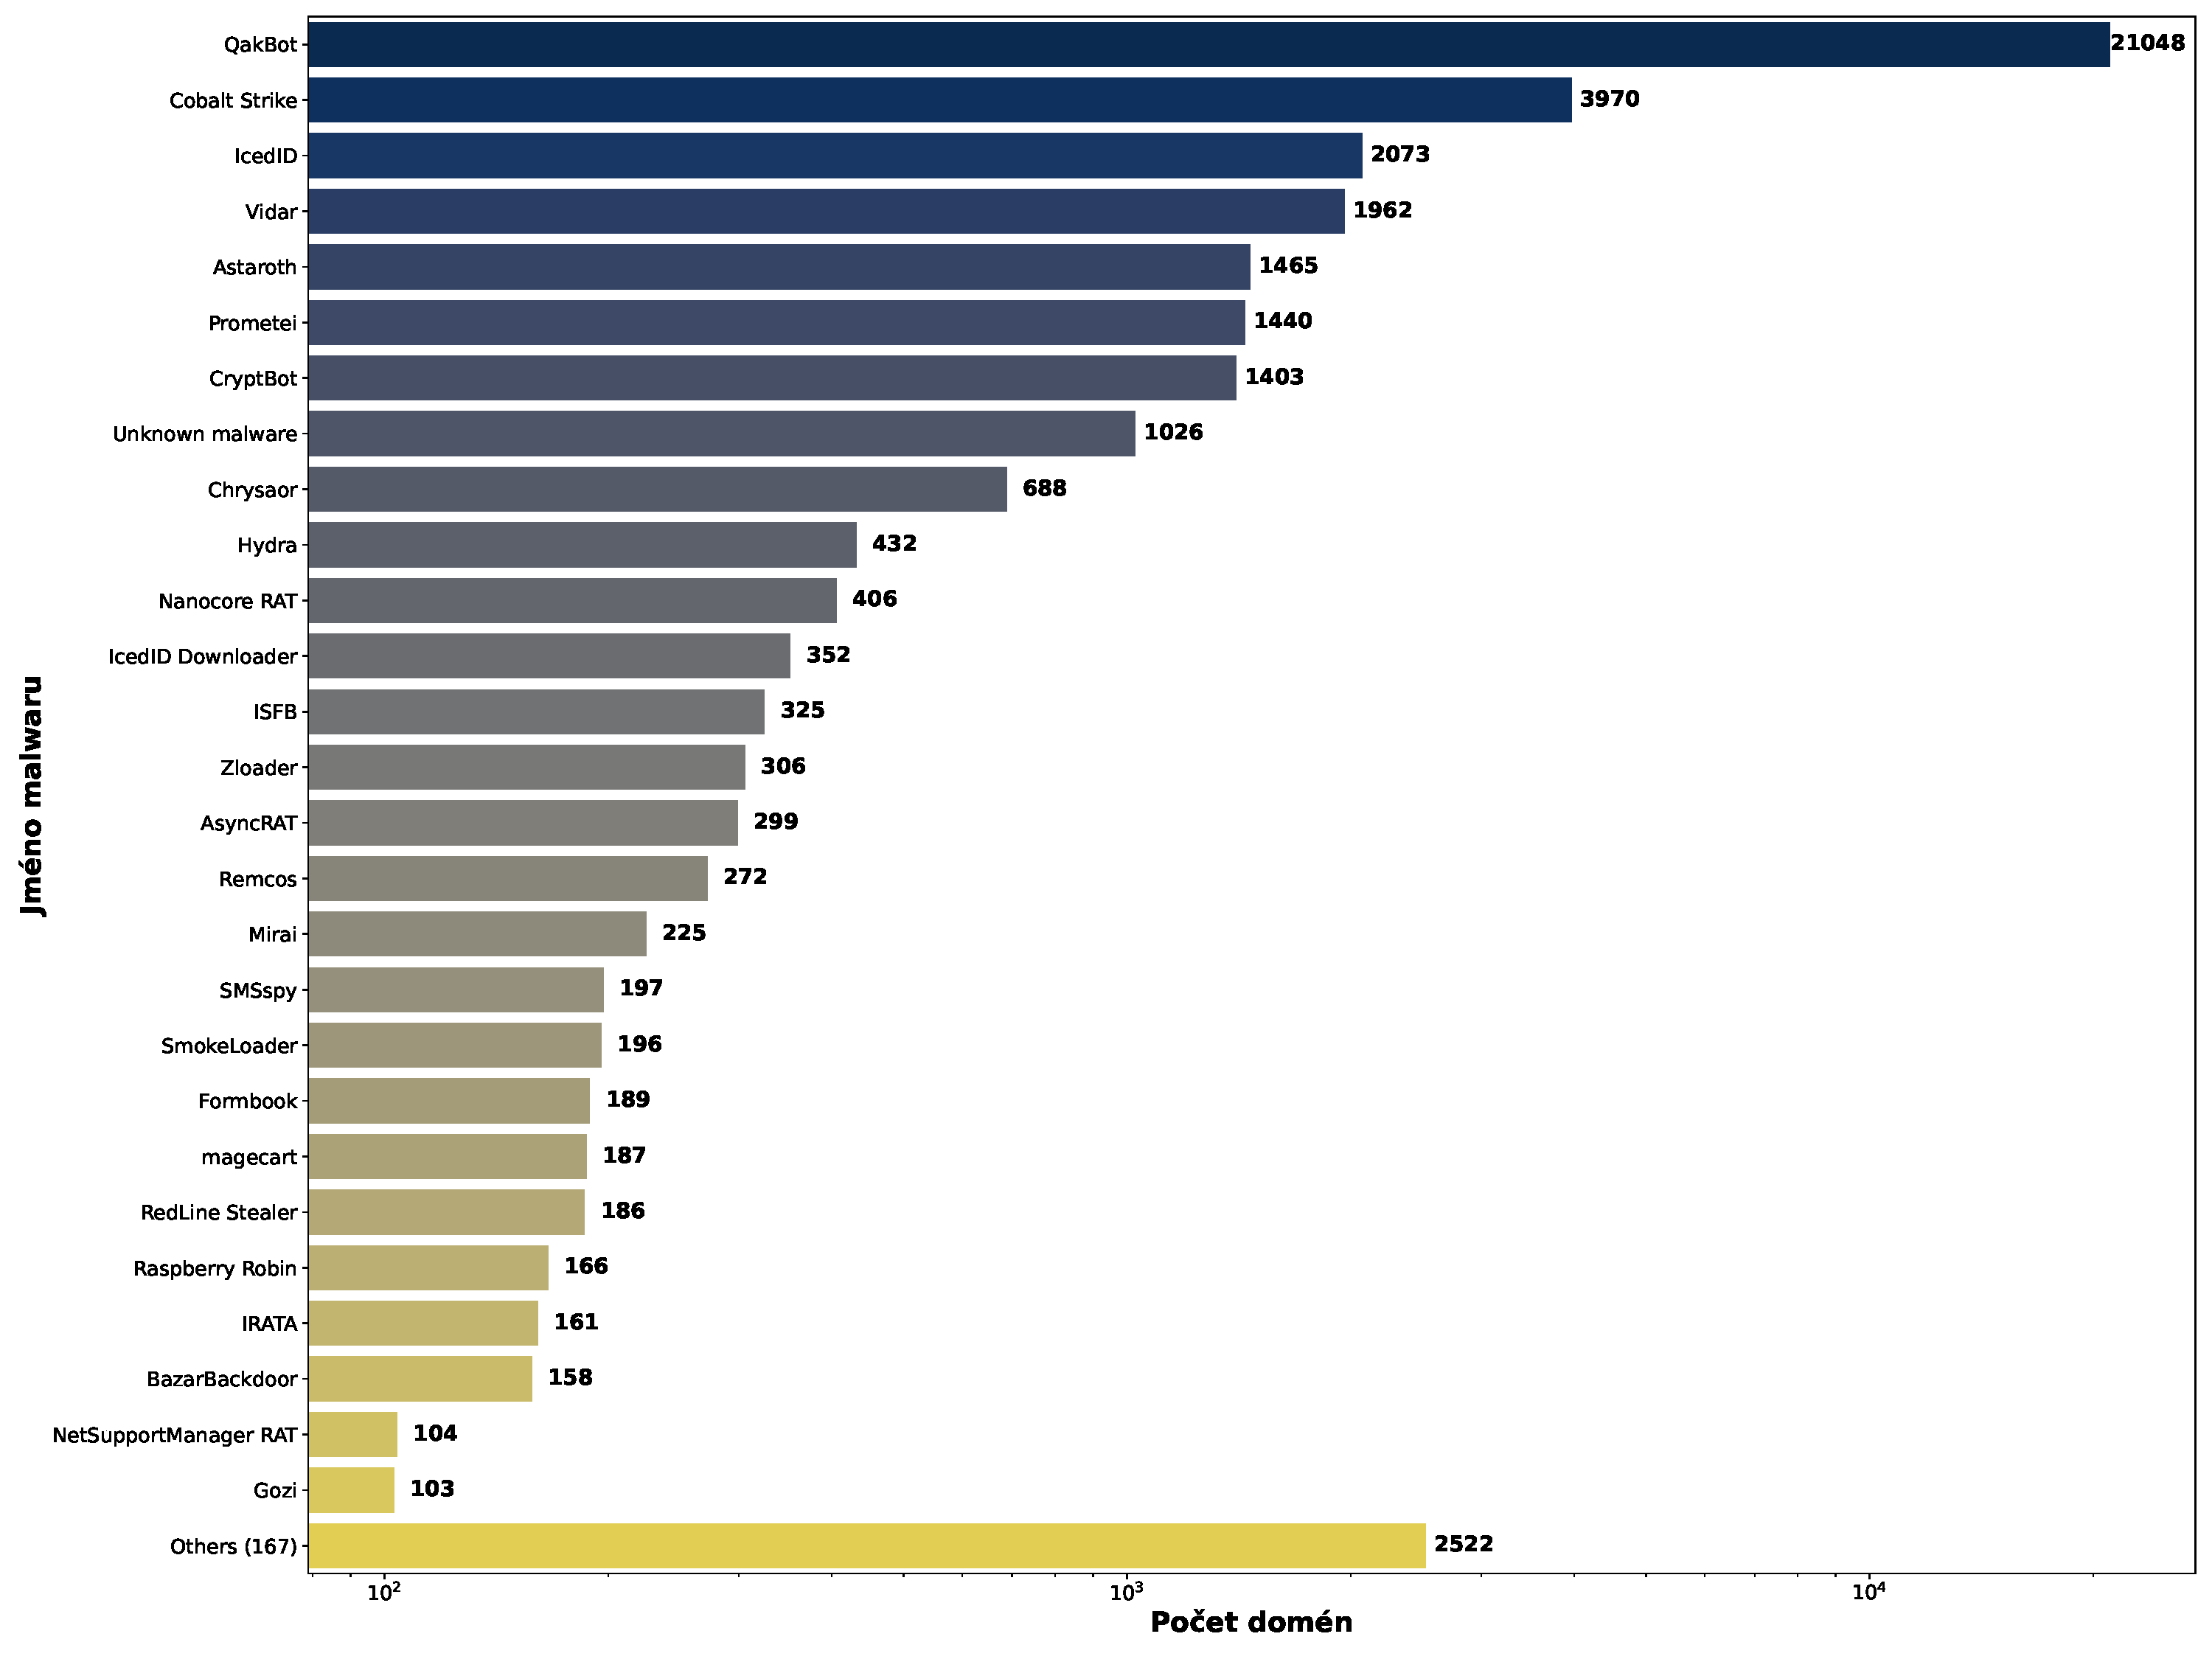
\includegraphics{obrazky-figures/malware_types_barplot.pdf}
            }
            \label{fig:malware_types}
    \end{figure}
\end{landscape}
  \fi
  
  % Kompilace po částech (viz výše, nutno odkomentovat)
  % Compilation piecewise (see above, it is necessary to uncomment it)
  %\subfile{xebert00-30-prilohy-appendices}
  
\end{document}
